% this main.tex largely serves to boot up all the packages and tie the various files together 

% add 'twocolumn' as an option in [] to get two columns, if you want
\documentclass[12pt,oneside,a4paper]{report}


% PACKAGES --------------------
% if this becomes too much, full install of latex, put in filename.sty in same folder as main.tex
% include \ProvidesPackage{packagename} and use usepackage{that} here

\usepackage[english]{babel}
\usepackage[utf8]{inputenc}

%next 4 lines suppress "Chapter N" etc. which is obnoxious
\usepackage{titlesec}
\usepackage{lipsum}

\titleformat{\chapter}[display]
{\normalfont\bfseries}{}{0pt}{\Large} %or {\Huge}

\usepackage{graphicx}  % use this to handle images

%FIXME!! GRAPHICSPATH DOESNT WORK
%\graphicspath{ {/home/pat/heme-binding/thesis/figures/} } % specify path to images
\graphicspath{{./figures/}}
%\makeatletter\typeout{\Ginput@path}\makeatother
%\graphicspath{c_Back_Matter/figures/}
% none of these work. manually specifying figures/figuretitle works...


%\usepackage{xcolor}
% for the uh, apparently American style of quotation marks
\usepackage [english]{babel}
\usepackage [autostyle, english = american]{csquotes}


% for the page number problem
\usepackage{fancyhdr}

\fancypagestyle{plain}{%
	\fancyhf{}
	\fancyfoot[C]{\iffloatpage{}{\thepage}}
	\renewcommand{\headrulewidth}{0pt}}
\pagestyle{plain}



\MakeOuterQuote{"} % or `` and " or ` and '


\usepackage[toc,page]{appendix} % for the appendix ofc.

\usepackage{subfig} %idk why this one is brackets lol just based off stackexchange


%=== WARNING %===: IF ISSUES PRESENTED WITH BIBLIOGRAPHY, IN TERMINAL, IN DIRECTORY OF MAIN.TEX, RUN THE COMMAND "biber filename" with no ext in filename.ext. If you run with .ext it will not work.
\usepackage[backend=biber]{biblatex} %enable bibliography
\addbibresource{ThesisReferences.bib}
 %auto-synced from Mendely Desktop, Thesis Refs.bib should auto update then get input to here etc.

% for kable/tables??
\usepackage{booktabs}
\usepackage{longtable}
\usepackage{array}
\usepackage{multirow}
\usepackage{wrapfig}
\usepackage{float}
\usepackage{colortbl}
\usepackage{pdflscape}
\usepackage{tabu}
\usepackage{threeparttable}
\usepackage{threeparttablex}
\usepackage[normalem]{ulem}
\usepackage{makecell}
\usepackage{xcolor}


\usepackage{rotating}
%%% LOTS OF GARBAGE %%%%%%


%\usepackage{blindtext} %idk
%\usepackage{algorithm2e}
%\usepackage{float} %to list algorthims

% GLOSSARY, IF DESIRED. **MUST GO HERE, or before begin document in main** ------------
% LIKELY REQUIRES FULL LATEX INSTALLATION LOLLOLLOLOL

%\makeglossaries
%\makenomenclature
%\makeindex[columns=3, title=Alphabetical Index, intoc] % Make LaTeX produce the files required to compile the index

%\loadglsentries{C) Back Matter/acronyms.tex}
%\loadglsentries{C) Back Matter/glossary.tex} 
%\makeglossaries %https://www.overleaf.com/learn/latex/glossaries


% note: title info in title.tex in A) Front Matter


% LOAD LAST. THIS PACKAGE IS SUPER MEGA IMPORTANT YO, OTHERWISE NO %STRUCTURE!!!!!
\usepackage{subfiles}

% END OF PACKAGES --------------




% STRUCTURE OF THE DOCUMENT ---------------
\begin{document}
	% ENGAGE TITLE PAGE
	\title{attached title}
\author{Pat the Great and Powerful}
\date{29 June 2021}
\maketitle
	
	\chapter*{Abstract}
	
	
		%not sure why I can't just \input abstract but w/e
		Metalloproteins compose approximately 40 percent (look up how to do percents in latex) of all known proteins, and use some metallic group to accomplish their chemistry. One such metallic group is heme. Heme is a member of the porphyrin family, which are able to catalyze a broad range of reactions. Heme in particular catalyzes many different reactions and is present in many proteins. However, the underlying structural requirements to host heme in a protein are not well studied.
		
		In this study, all heme or heme-c containing proteins as of xx were downloaded and processed in order to determine underlying structural characteristics these proteins may have in common. Parameters that were examined include: xx. Overall, we found: xx. These results may have implications for protein engineering; or if I fucked up this illustrates the difficulty of the field and demonstrate the wide range of acceptable environments of heme; it may therefore be more appropriate to take a more hands-on approach until perhaps other computational methods evolve to better examine structure-function relationships.
		
		See? Not so bad of a worst-case scenario. Just, an unusual sentiment to see in modern science.
		
	
	\chapter*{Lay Summary}
		
		Proteins are biological molecules that perform essential functions in our bodies and in all living things. They are responsible for everything from transporting oxygen in our blood to photosynthesis in plants. They can be extracted from living things and cultured in laboratories and factories. They can then be used as drugs, or be used to perform functions in industrial processes.
		
		Many proteins require additional molecules to perform their function, and these molecules must be bound, docked to the molecule like a boat in a harbor. The molecules can be bound to the protein inside a specialized space, or pocket, within or on the surface of the protein.
		
		One class of proteins is hemoproteins - proteins that use the molecule heme to perform their function. The heme is critical to the proper function of these proteins. Heme enables many specific chemical reactions to be performed, or assisted by the protein. In hemoglobin, in blood, the heme molecule allows the overall protein of hemoglobin to carry and transport oxygen around the body.
		
		But the specifics of the pocket that binds heme in these hemoproteins is not well understood. What are the conditions inside the pocket? Is it a very specific size or can it vary? Is there anything in common among the pockets of many different hemoproteins? These are the questions this research hoped to answer; or at the very least, provide some data and lay the groundwork for others to continue the research later.
		
		This investigation was not conducted in a lab. Rather, using various software packages and the 3D structures of hemoproteins published in a database, various properties of these hemoproteins were calculated. The data produced were analyzed with various statistical methods to extract potentially useful information.
		
		Overall, the following was found:
		%probably use a bullet list, maybe
		Grad school sucks but bravas are delicious.
	
	\chapter*{Acknowledgments}
	
		In case anyone reads this in the future, some context may be appreciated: I attended and completed this Master's during the COVID-19 global pandemic from September 2020 to September 2021.
		
		Thanks professors
		
		Thanks lab
		
		Thanks UAB
		
		Thanks Spain, and Catalonia, allowing me in and then also having public health measures unlike Donny's America
		
		Thanks classmates
		
		Thanks fam, friends
		
		Thanks to the media and the creators of media that facilitated the survival of my sanity through the pandemic.
		\\~\\
		Finally, I'd like to quote a well-known artist from California. He was referencing his own work, but I wholly identify with his appreciation for the subject of his esteem:
		\\~\\
		"Last but not least, I wanna thank me. I wanna thank me for believing in me. I wanna thank me for doing all this hard work. I wanna thank me for having no days off. I wanna thank me for, for never quitting. I wanna thank me for always being a giver, and trying to give more than I receive. I wanna thank me for trying to do more right than wrong. I wanna thank me for just being me at all times."
		
		-- Calvin Cordozar Broadus Jr.
		
		%https://www.youtube.com/watch?v=NfF3bThOW0Q
	
	
	%BLANK PAGE
	\chapter*{}
	%TOC
	\tableofcontents
	\listoffigures
	\listoftables
	
	\pagebreak
	
	%%%==== MAIN MATTER ====%%%
	
	%listing chapters in order, avoid need to rename numbers if start moving things around/remove equipment chapter
	
	\chapter{Introduction}
	
	*insert the abstract's first paragraph basically here later
	
	In previous work, only ~125 hemoproteins were studied. Although pdbs were thoroughly examined and the datasets were culled, the sample size of this study is very small compared to the amount of hemoproteins available in the pdb a decade later (~10,000 HEM-containing proteins and xx). While not possible to cull as in this study, the additional sample size is of interest to examine for other structural motifs or underlying characteristics.
	
	These characteristics include: xx. They are achieved by either scanning the pdb for them or calculation as detailed below. 
	
	All of these characteristics have implications in the field of protein engineering or basic research into hemoproteins. Examples of the uses of these results include [SUPER BLOOD STUDY] and [OTHER PROTEIN ENGINEERING STUFF]. Not sure how much we can reference those other papers besides doing that besides in the conclusion.
	
	Notable results from some of the prior studies include: xx and xx. These characteristics are also examined in this dataset, while some are not due to different study approaches. 
	
	\chapter{Methods}
	% see in Project bookmark folder for multiple columns in your doc, broken up by section:
	% https://tex.stackexchange.com/questions/17949/twocolumn-part-in-document
	
	
	\section*{Datasets}
	**Remember to alter how this header's size appears... later.
	Several datasets were constructed to examine the full ... (this sentence belongs in the intro, I think)
	The primary dataset of heme-containing proteins (HEM) was composed by finding approximately 30 (specify exact number) of types of proteins that are present in the PDB. This included heme oxygenase, myoglobin, cytochrome P450, among many others.
	
	Datasets: HEM, HEC(?), SRM, VER/VEA.
	
	Four datasets were constructed for this study.
	
	The primary dataset of heme-containing proteins (HEM) was constructed by searching for 30 different classes of proteins; this enabled a dataset of diverse proteins to account for any structural deltas to achieve different chemistry. Additional samples of each class of protein were then added to the dataset, bringing the total to XX. The PDBs were restricted to the following criteria to ensure quality: XX. A full list of proteins and their source organism used in the study is available in table XX.
	
	The heme-c dataset followed the same criteria (XX). Similar proteins were searched for as HEM, depending on availability in the PDB/possibility with chemistry. This dataset was anticipated to be fairly similar to HEM, and so only contains XX samples. The full table is available in table XX. 
	
	The siroheme dataset (SRM) contains fewer samples than HEM or HEC due to the limited structures available. A search for 'SRM' as of 26 July 2021 produced 52 structures. Not all of these structures contain siroheme. A full-text search for "siroheme" produces many more results, but very few are complex with siroheme. SAH appears commonly used to complex the relevant siroheme proteins, however examination of whether this guarantees acceptable results/estimates of SA/V etc. is outside the scope of this study. No quality criteria were employed, but all proteins are within: XX.
	
	The verdoheme dataset (VER/VEA) is very limited. A search for "verdoheme" as of 26 July 2021 produces 12 results. From these results only 4 usable proteins are available. All PDBs fall within XX criteria. 
	
	
	Some PDBs in HEM-dataset contain PDBs where there is a double-molecule representation of heme. If this has not been taken care of ** FIX ME!!!* then write something here.
	
	The scripts used in this study were modified depending whether HEM/HEC/SRM/VER/VEA were being processed, and depending on the distance from the ligand of interest being examined (i.e. 5-7A). This is discussed in further detail below MAYBE (FIXME!).
	
	\section*{Confirming data quality and details/PDB detail table}
	All PDBs used in the study were scanned/text-parsed with a python script. This script grabbed a bunch of relevant qualities, like molecule purpose, source organism, resolution (XX FIX), and PDB code to confirm. The data produced are in table X. 
	%this last line will likely be repeated a bunch so maybe just note it at the begining or below. yeah it's above, last line in previous section.
	
	\section*{Preprocessing/before chimera/monomers}
	Many of the PDBS downloaded are multimeric structures. These were all processed into monomeric structures, by selecting a single chain (chain A) and eliminating all others chains in each PDB. This makes examination easier and more representative when data are aggregated; multimers with more pockets would otherwise skew the data and be the majority represented in the results. 
	
	All scripts below were paused while running for visual examination; in rare cases the process of conversion to monomers resulted in errors processing, especially for volume measurements. This is discussed below if this issue was not corrected (FIXME!! XX).
	
	\section*{Examination in Chimera/acquiring results}
	Multiple scripts were written and applied in Chimera. These scripts are divided up based on what results are produced. 
	
	In the scripts the choice of 5A or 7A as a distance from the ligand is arbitrarily chosen. This is a distance that generally accounts for all residues able to interact with the ligand. The results are presented in both 5A and 7A sets to account for the variability introduced by these cutoffs. 
	
		\subsection*{Volume}
		
		Volume of the binding pockets for each ligand are calculated using surfnet. Atoms within 5-7A of the ligand are selected and the pocket volume they form with the ligand is calculated. The surfnet algorithm works by... making triangles along the molecular surface, I guess, until the distance cutoff.
		
		Volume of the ligands is also calculated, using a different method; the above method with surfnet is not possible to employ for single molecules outside the pocket. First the ligands were isolated from their pdb. The molecular solvent/surface area was calculated (Accesible and excluded). The surface area and the volume of the resulting... blob, is given by Chimera. This is not the same method as employed by surfnet to acquire volume and represents a limitation in the study (FIXME! IDK IF THIS SHOULD GET DISCUSSED HERE)
		
		Images of this operation are available in XX.
		
		\subsection*{Surface Area}
		Surface area of the pockets is calculated using a similar method as above. The atoms within 5-7A of the ligand are selected. The 'surf' operation is applied. This creates a surface... IDK how this algorithm works (FIXME!). Both accessible and excluded solvent area are outputted.
		
		Surface area of the ligands is calculated as noted above in Volume section.
	
		Images of this operation are available in XX. 
		
		\subsection*{Distances}
		
		Distances (NOT THE ANGLEDIST stuff) were calculated by selecting all atoms within 5-7A of Fe in the ligands. Each atom's distance to the Fe was calculated by using the distance operation in Chimera (confirm this is precisely what we do), which simply draws a line between the atom and the Fe atom. (FIXME! IN DISCUSSION, DISCUSS WHY METAL COORDINATION IS GARBAGE) 
		
		%%%%% FIXME Must redo this part in R and get the relevant data lollollololol
		The residue each atom is in is reported. Therefore, each
		
		\subsection*{Angles Residues - Heme Plane}
		
		\subsection*{Angles Fe-CA-CB}
		
		\subsection*{Amino Acid Frequency in Pockets}
		
		\subsection*{title}
	
	
	\section*{Importing to R and stastical analysis}
	
	FIgures wer also made in R. 
	
	
	\begin{itemize}
		
		
		
		
		\item Download from PDB using the script they’ve provided at RCSB for many, many files
		
		\item Use UCSF Chimera to determine:
		\begin{itemize}
			\item Volume
			\item SA
			\item Nearby AA
		\end{itemize}
		
		\item R to process raw data and produce tables
		\item Whatever other software we use to achieve the other results. E.g. E, or availability to solvent etc. likely will stick w Chimera I suspect. Or somehow implement the Python script to open both chimera for the first part of what we’ve done or for something else later. The script we’ve written is a python script, not a chimera script. We’re initializing it with chimera and excluding the necessary code… to initialize chimera and specify chimera to receive the commands
		
	\end{itemize}


	%add something like see pat's github for algorithms in methods
	\chapter{Equipment}
	\chapter{Results}
	\chapter{Dicussion}
	\chapter{Conclusion}
	this is just as master’s and in basic research don’t feel the need to replicate what took some god forsaken, sad, overworked, impoverished PhD students years + with help of their PIs and with generous word fluff to hide fuck ups. 0 -> thesis in approx. 3-4 months during global catastrophe is nifty
	
	\printbibliography % by convention, references before appendices
	
	
	
	\begin{appendices}
	%uncomment next line if you wish section names not to appear in toc
	%\addtocontents{toc}{\protect\setcounter{tocdepth}{0}}
	
		\chapter{Figures}
			\section{AA Frequency}
	%NOTE!!! that due to figures.tex's file position, we are in working directory /figures/
	

	\begin{figure}
		\caption{HEM AA Frequency 7A}
		\label{figs:HEM_aafreq7}
		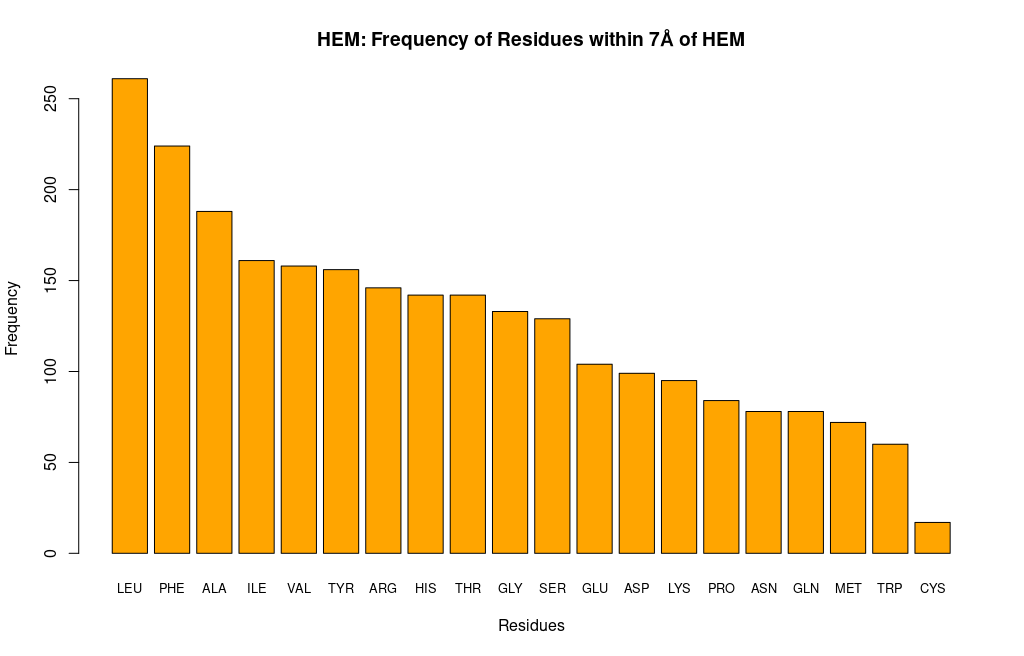
\includegraphics[width=1.0\textwidth]{7A/HEM_aaFreq}
		%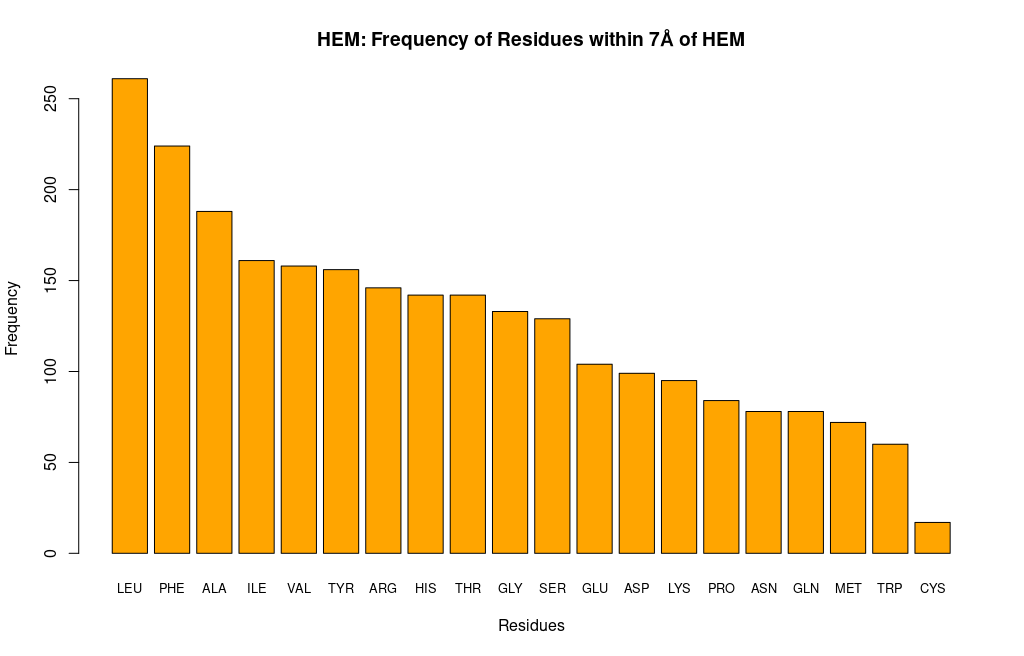
\includegraphics{~/heme-binding/thesis/figures/fuckinghell}
	\end{figure}
	
	\begin{figure}
		\caption{HEC AA Frequency 7A}
		\label{figs:HEC_aafreq7}
		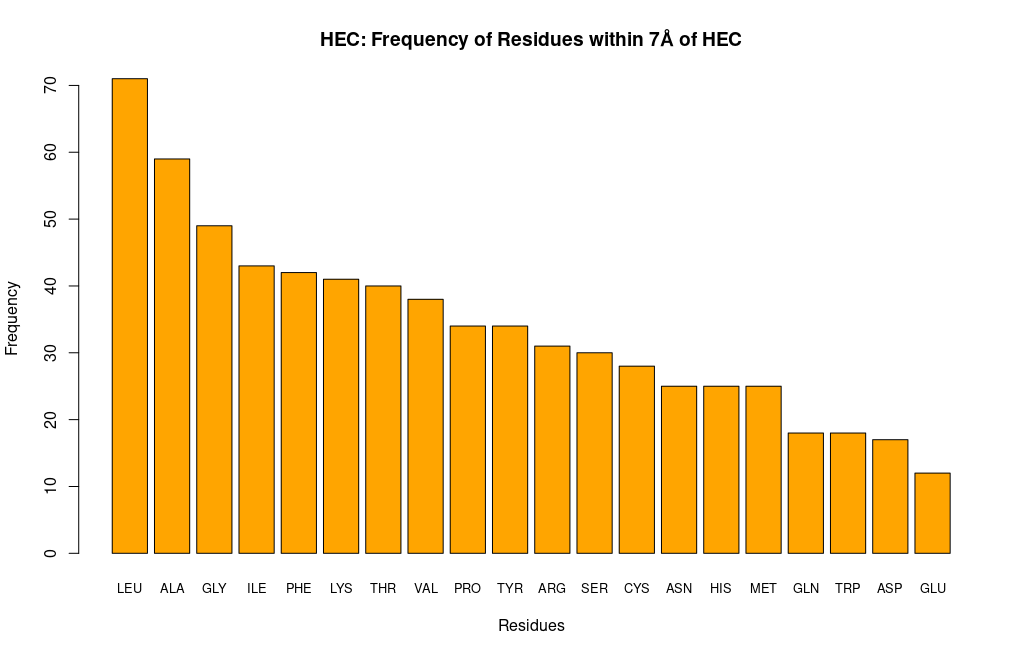
\includegraphics[width=1.0\textwidth]{7A/HEC_aaFreq}
	\end{figure}
		
	\begin{figure}
		\caption{SRM AA Frequency 7A}
		\label{figs:SRM_aafreq7}
		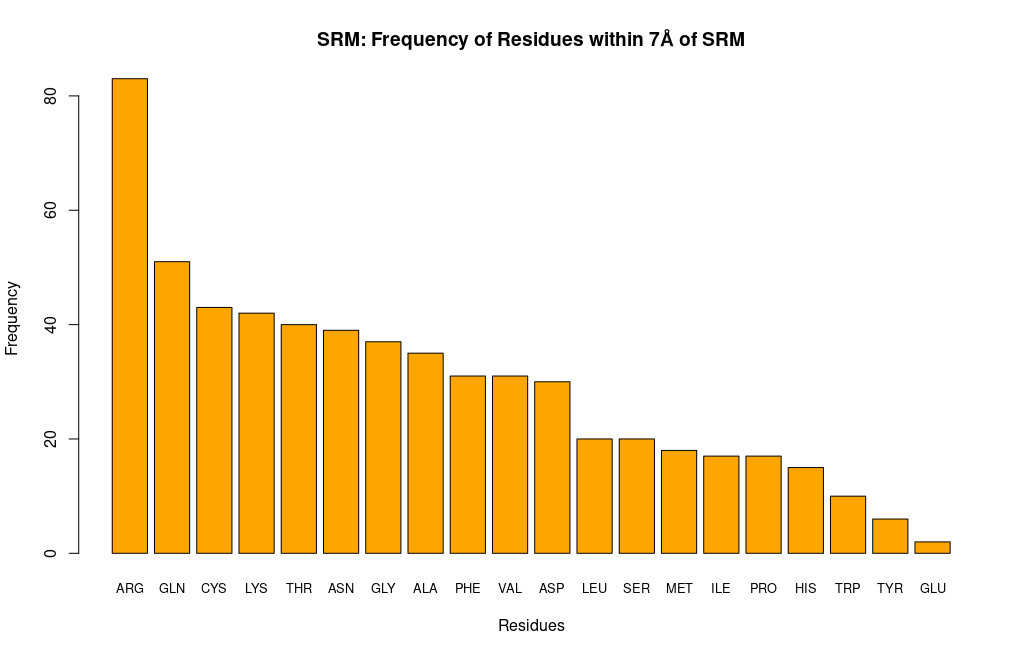
\includegraphics[width=1.0\textwidth]{7A/SRM_aaFreq}
	\end{figure}
	
	\begin{figure}
		\caption{VERDOHEME AA Frequency 7A}
		\label{figs:VERDOHEME_aafreq7}
		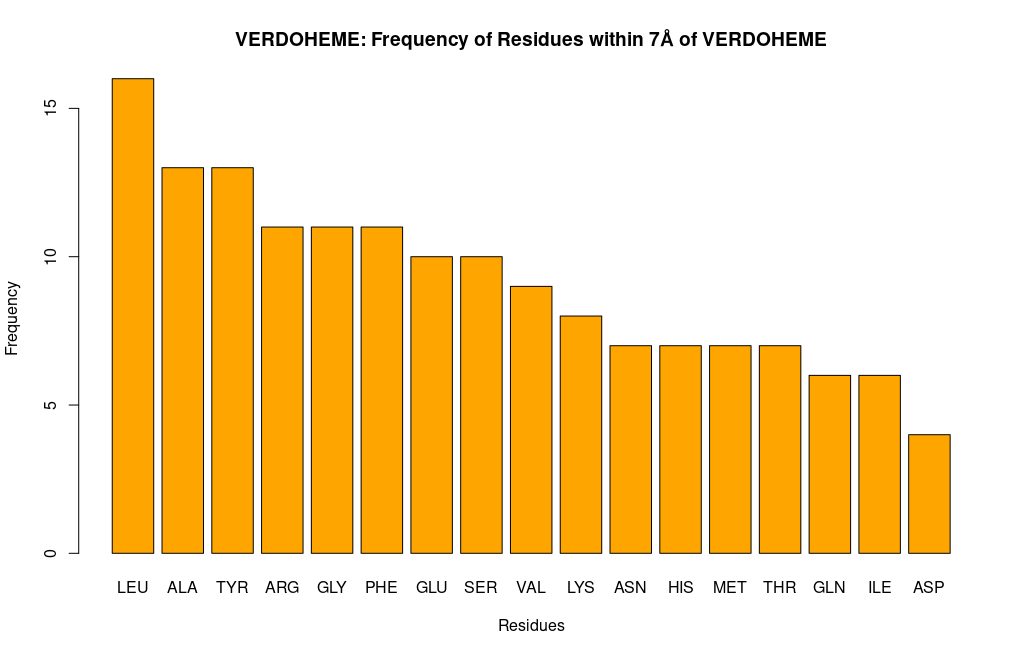
\includegraphics[width=1.0\textwidth]{7A/VERDOHEME_aaFreq}
	\end{figure}



		
\section{CACBFe Data}
	\begin{figure}
		\caption{HEM CACBFe Data}
		\label{figs:HEM_cab7}
		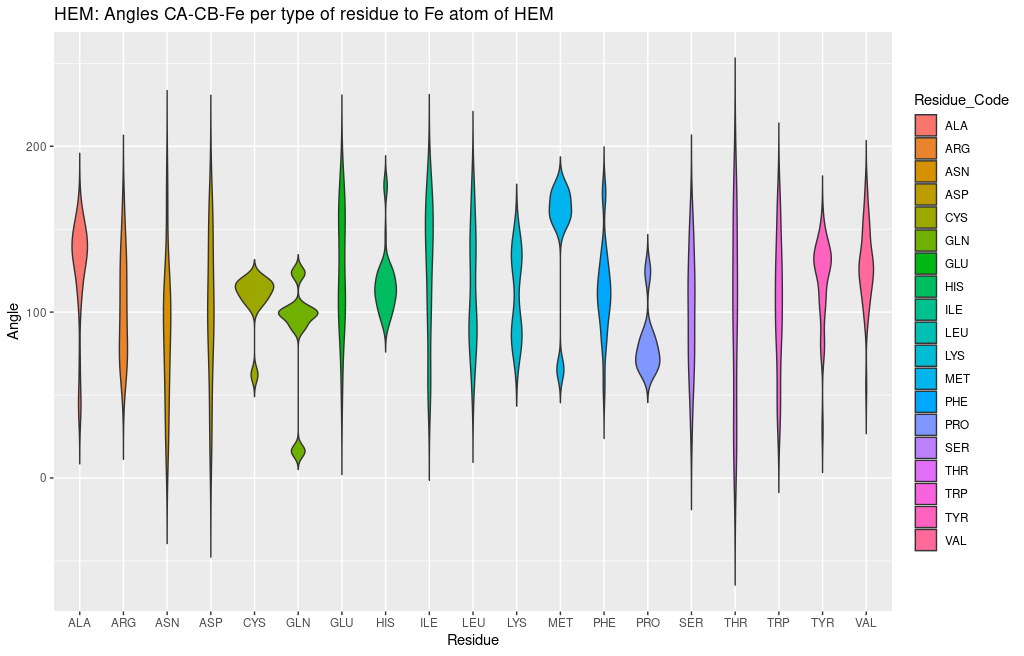
\includegraphics[width=\linewidth]{7A/HEM_cab}
	\end{figure}

	\begin{figure}
		\caption{HEC CACBFe Data}
		\label{figs:HEC_cab7}
		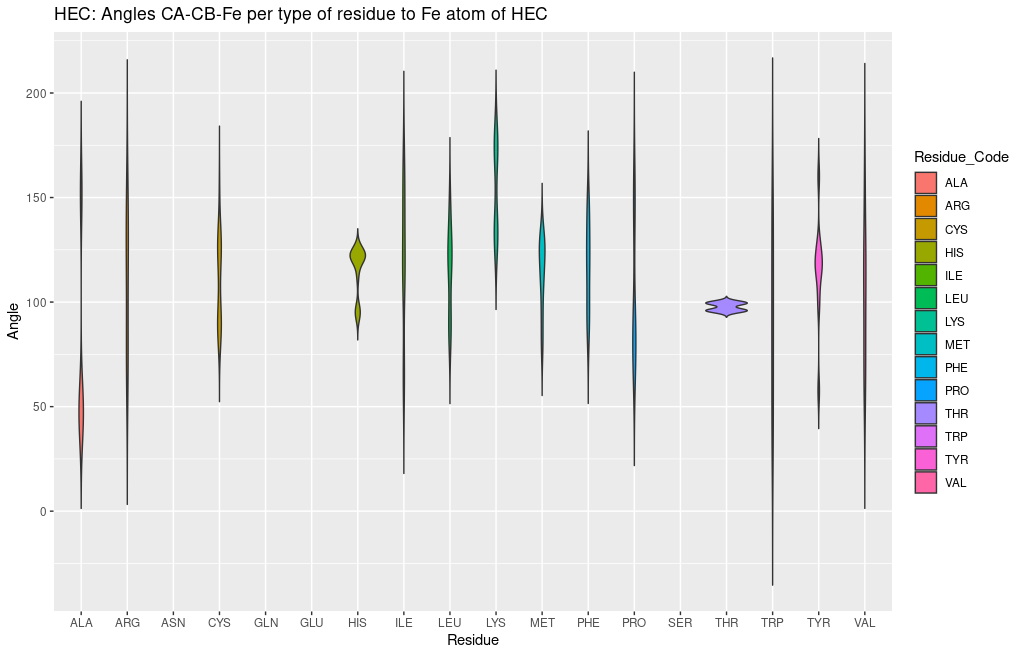
\includegraphics[width=\linewidth]{7A/HEC_cab}
	\end{figure}
	
	\begin{figure}
		\caption{SRM CACBFe Data}
		\label{figs:SRM_cab7}
		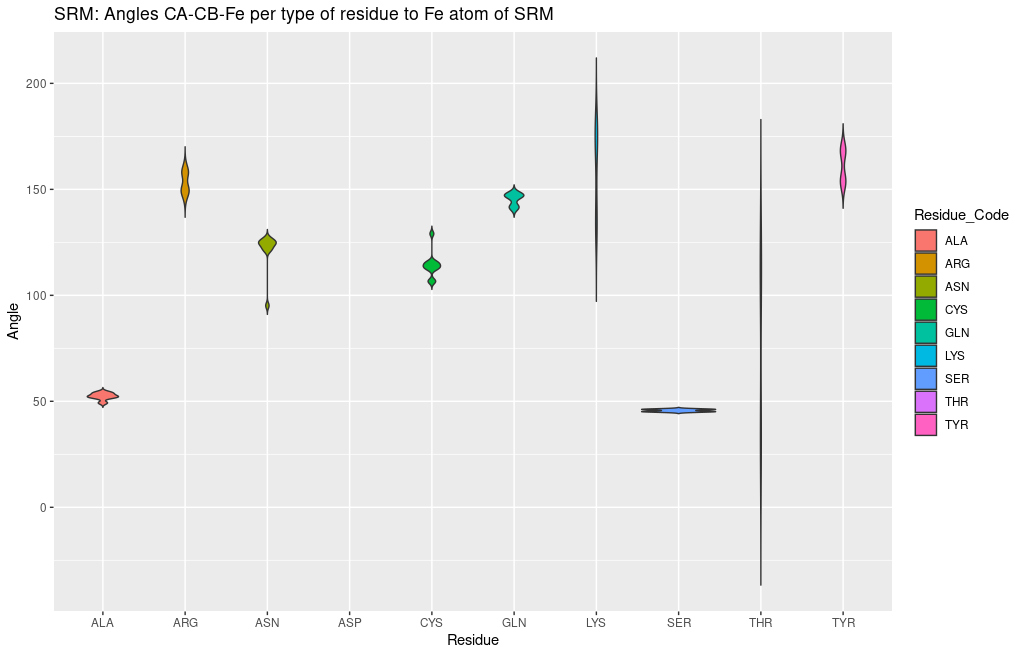
\includegraphics[width=\linewidth]{7A/SRM_cab}
	\end{figure}
	
	\begin{figure}
		\caption{VERDOHEME CACBFe Data}
		\label{figs:VERDOHEME_cab7}
		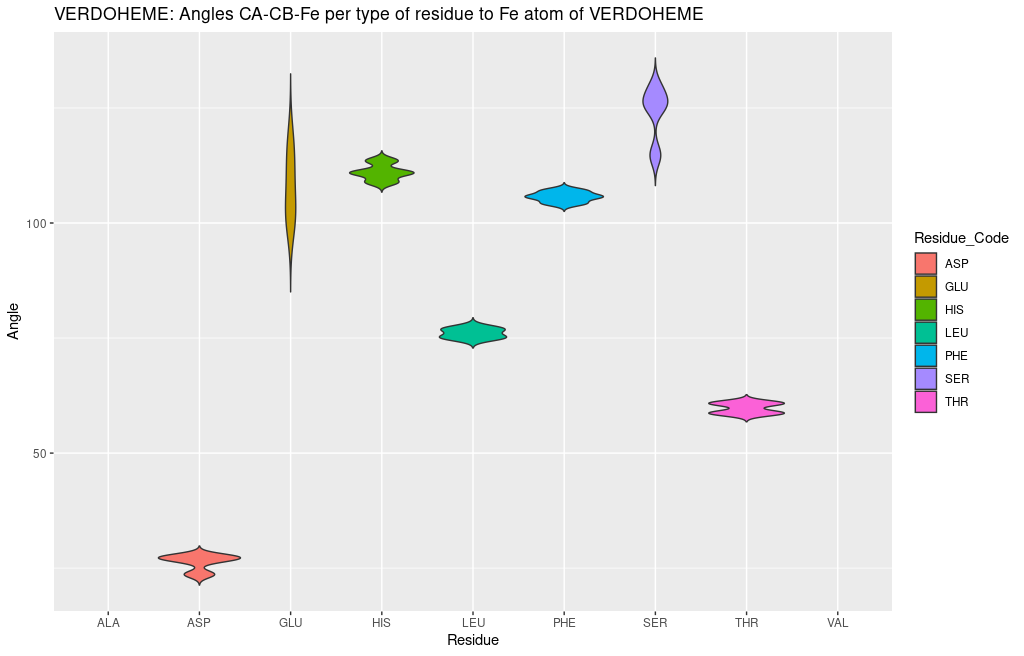
\includegraphics[width=\linewidth]{7A/VERDOHEME_cab}
	\end{figure}
	
\section{Closest Residue Data}
	\begin{figure}
		\caption{HEM Closest Residue Data}
		\label{figs:HEM_closestRes7}
		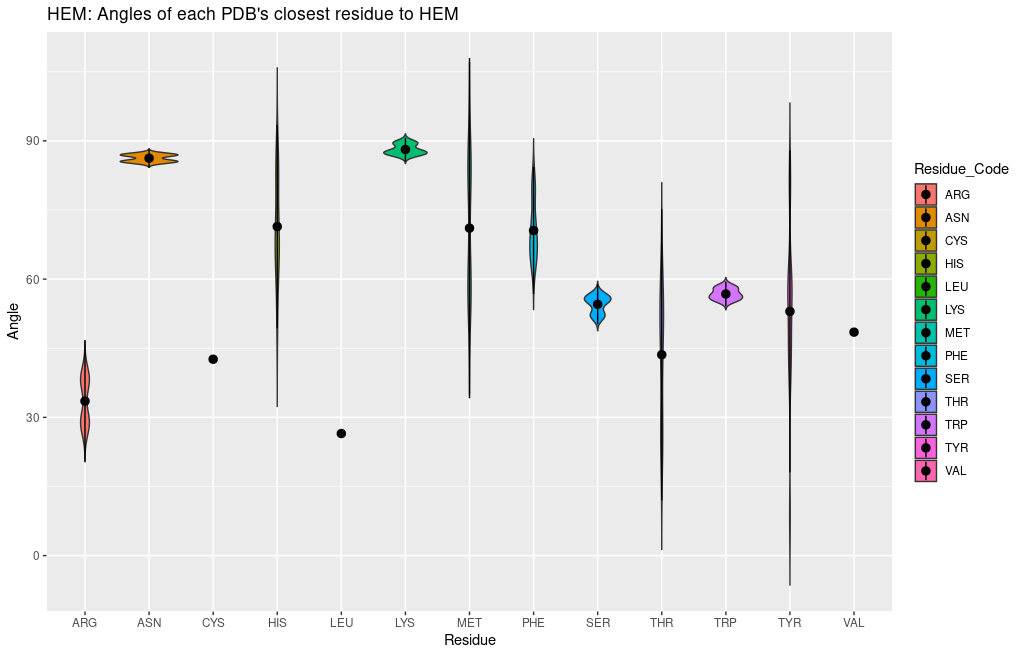
\includegraphics[width=\linewidth]{7A/HEM_closestRes}
	\end{figure}
	
	\begin{figure}
		\caption{HEC Closest Residue Data}
		\label{figs:HEC_closestRes7}
		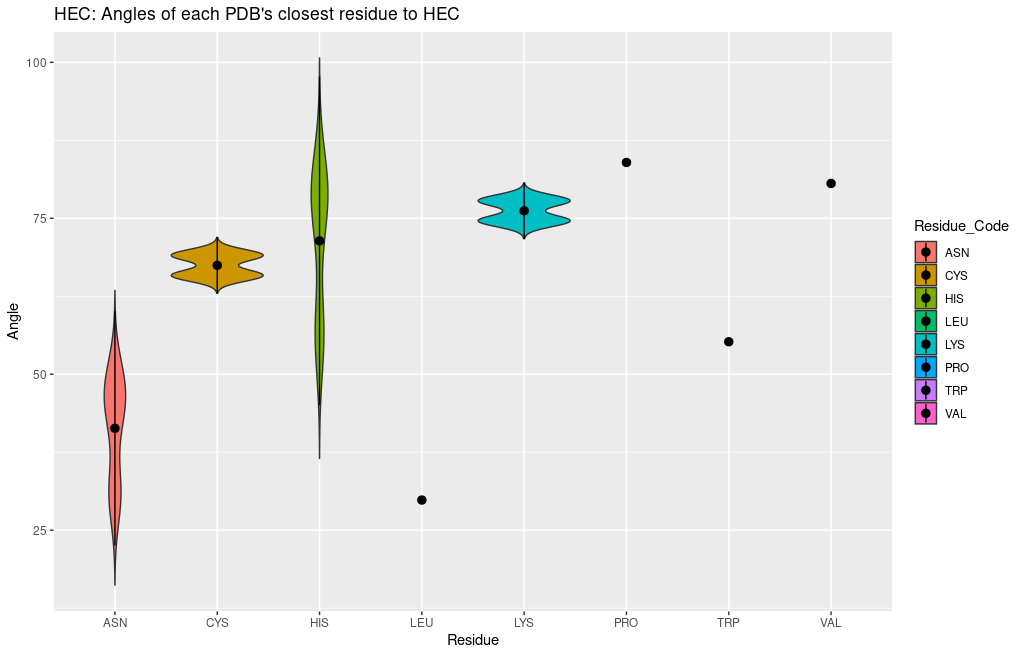
\includegraphics[width=\linewidth]{7A/HEC_closestRes}
	\end{figure}
	
	
	\begin{figure}
		\caption{SRM Closest Residue Data}
		\label{figs:SRM_closestRes7}
		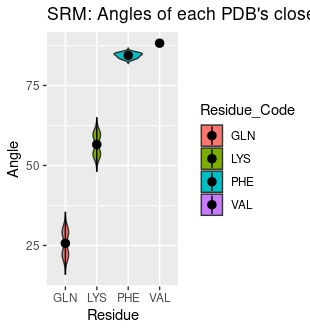
\includegraphics[width=\linewidth]{7A/SRM_closestRes}
	\end{figure}


	\begin{figure}
		\caption{VERDOHEME Closest Residue Data}
		\label{figs:VERDOHEME_closestRes7}
		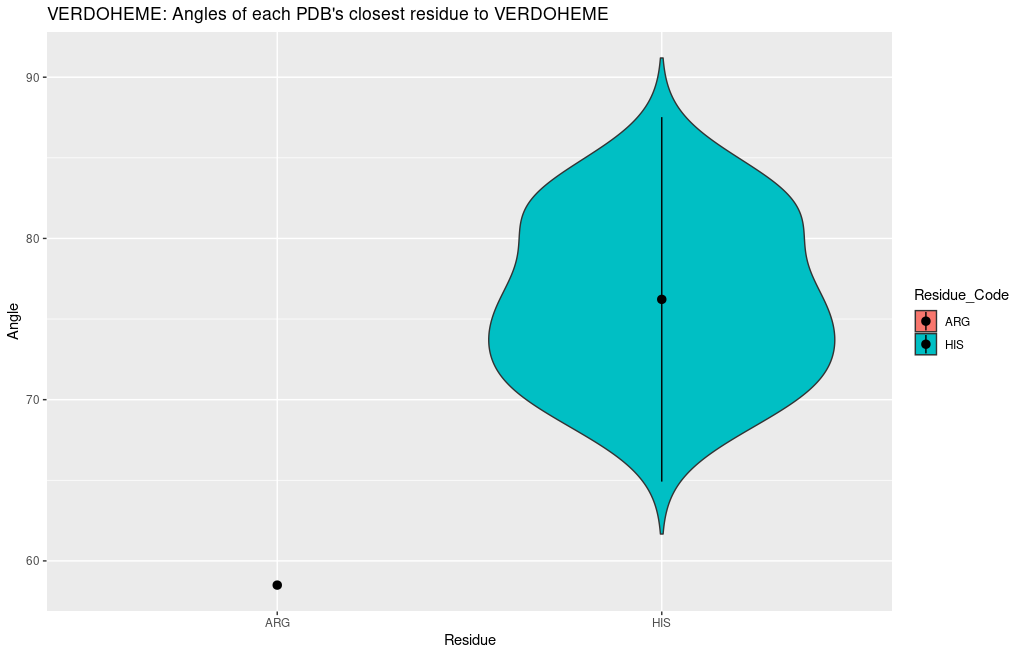
\includegraphics[width=\linewidth]{7A/VERDOHEME_closestRes}
	\end{figure}


\section{Coordinating Residue Data}
	\begin{figure}
		\caption{HEM Coordinating Residue Data}
		\label{figs:HEM_coordRes7}
		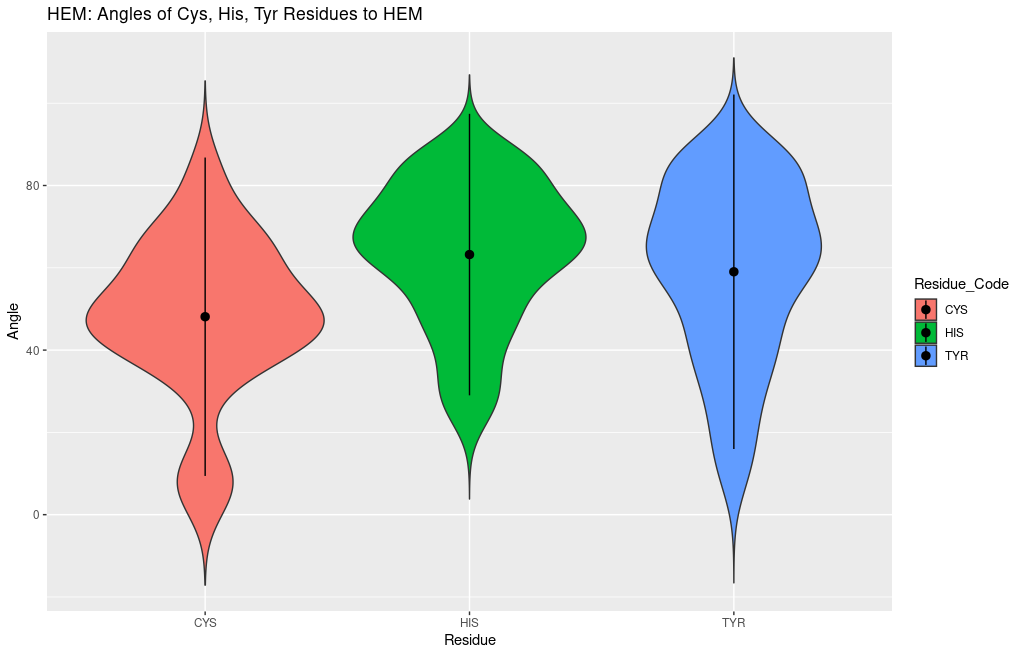
\includegraphics[width=\linewidth]{7A/HEM_coordRes}
	\end{figure}
	
	\begin{figure}
		\caption{HEC Coordinating Residue Data}
		\label{figs:HEC_coordRes7}
		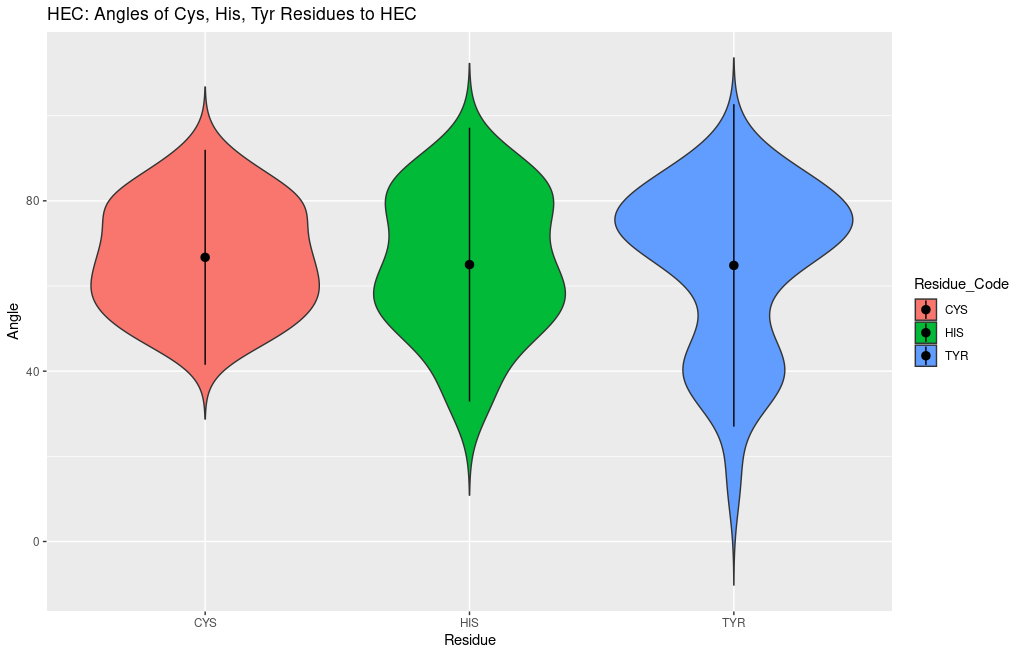
\includegraphics[width=\linewidth]{7A/HEC_coordRes}
	\end{figure}	
		
	\begin{figure}
		\caption{SRM Coordinating Residue Data}
		\label{figs:SRM_coordRes7}
		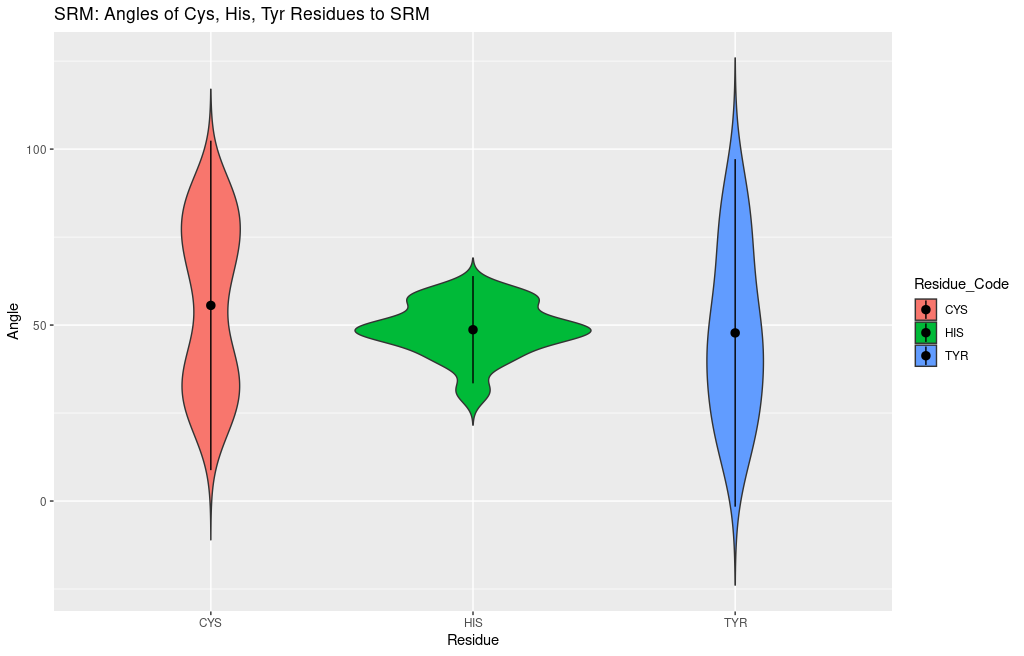
\includegraphics[width=\linewidth]{7A/SRM_coordRes}
	\end{figure}
		
	\begin{figure}
		\caption{VERDOHEME Coordinating Residue Data}
		\label{figs:VERDOHEME_coordRes7}
		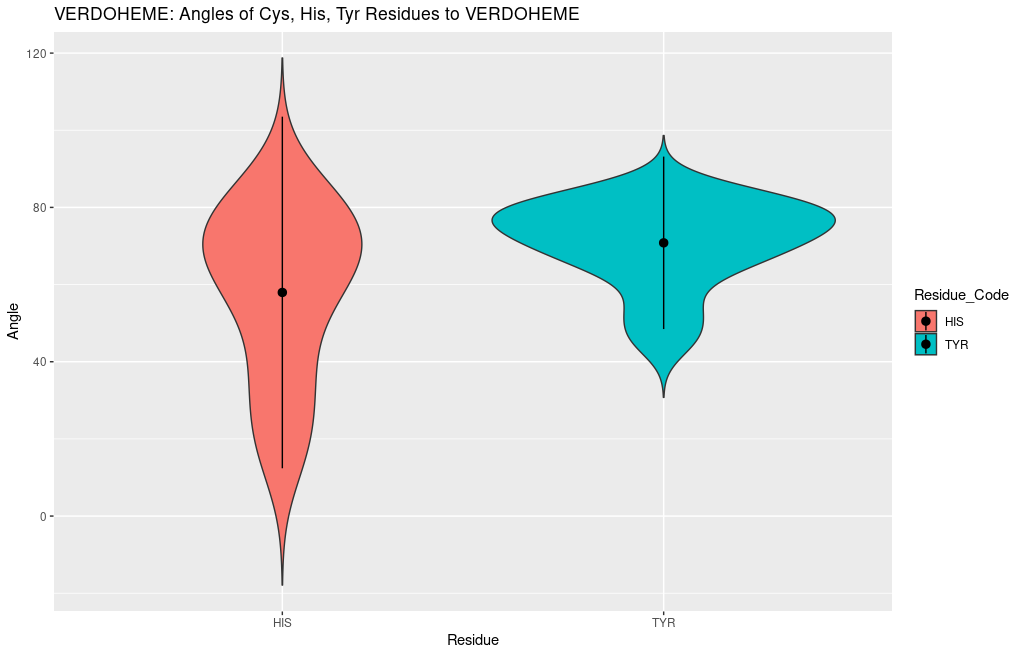
\includegraphics[width=\linewidth]{7A/VERDOHEME_coordRes}
	\end{figure}


\section{Ligand Accessible Surface Area}
	\begin{figure}
		\caption{HEM Ligand Accessible Surface Area}
		\label{figs:HEM_ligandAccSA}
			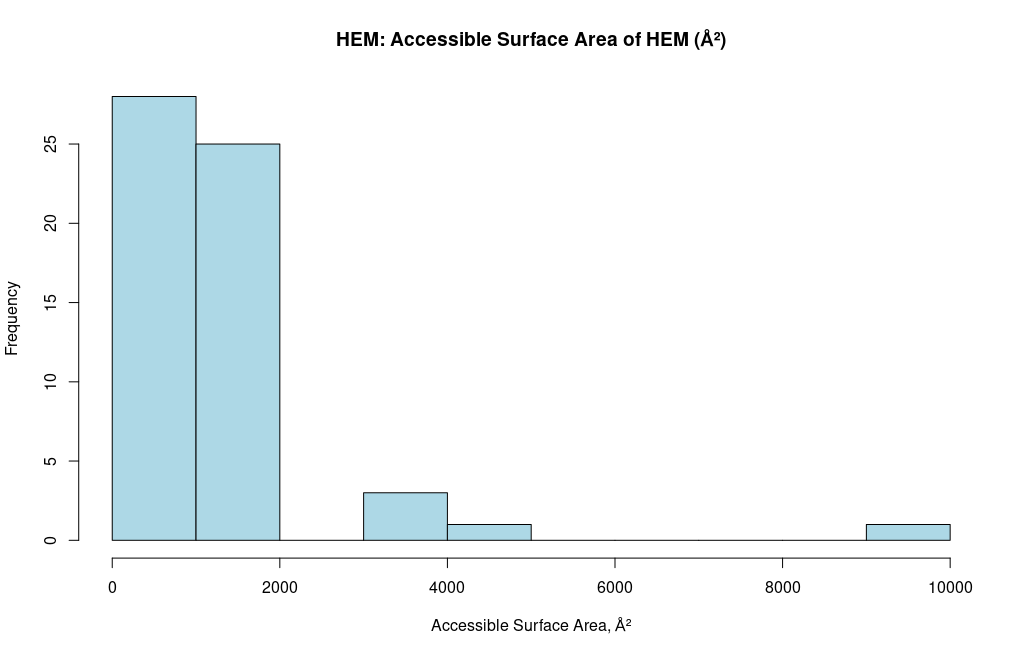
\includegraphics[width=\linewidth]{7A/HEM_ligandAccSA}
	\end{figure}

	\begin{figure}
		\caption{HEC Ligand Accessible Surface Area}
		\label{figs:HEC_ligandAccSA}
		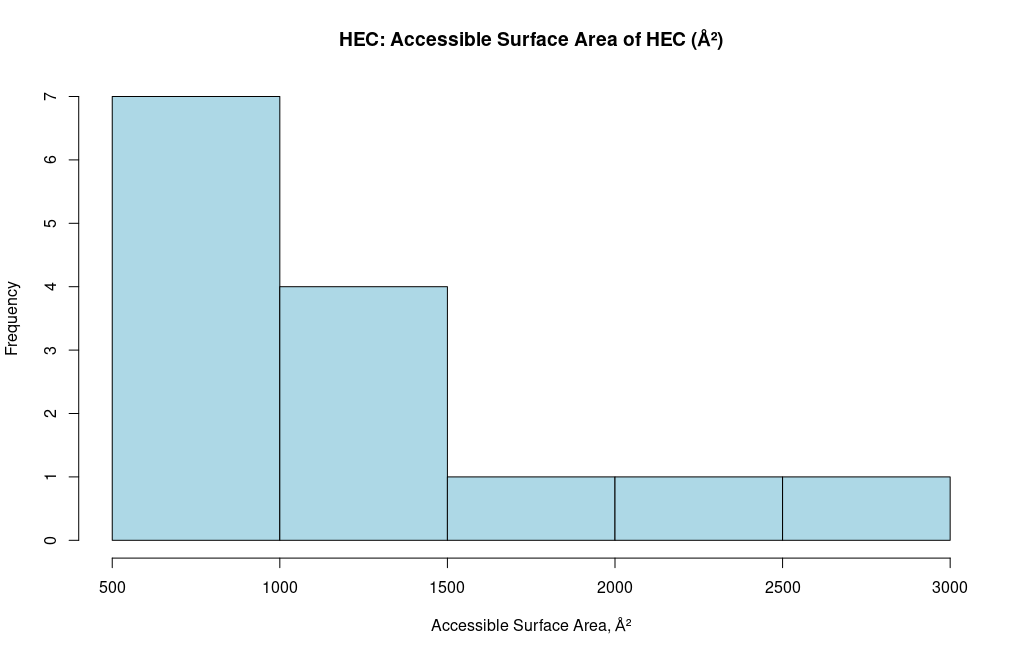
\includegraphics[width=\linewidth]{7A/HEC_ligandAccSA}
	\end{figure}

	\begin{figure}
		\caption{SRM Ligand Accessible Surface Area}
		\label{figs:SRM_ligandAccSA}
		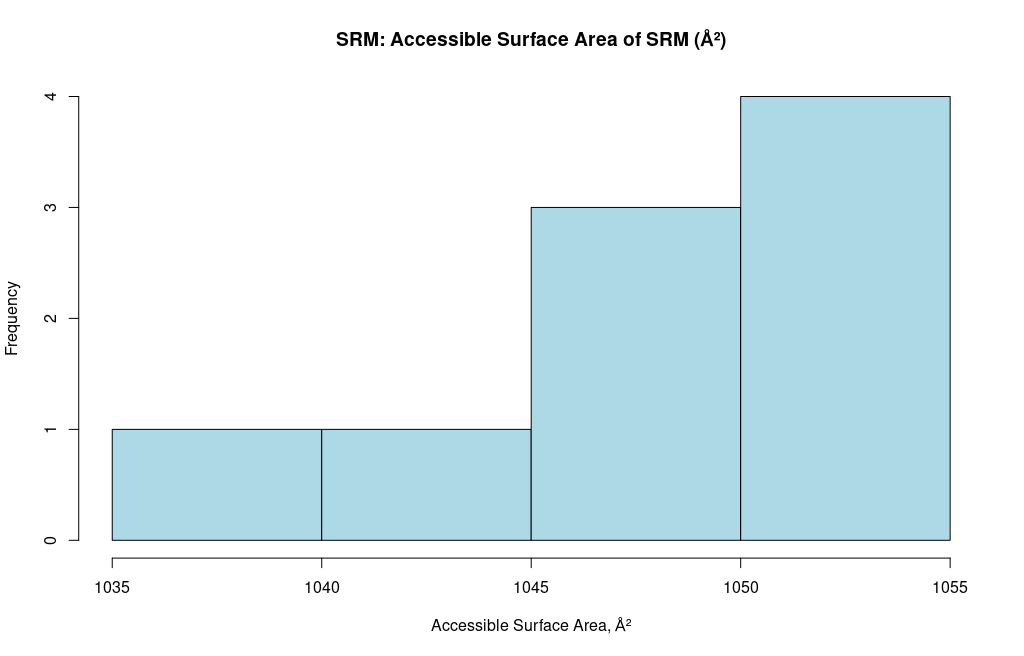
\includegraphics[width=\linewidth]{7A/SRM_ligandAccSA}
	\end{figure}

	\begin{figure}
		\caption{VERDOHEME Ligand Accessible Surface Area}
		\label{figs:VERDOHEME_ligandAccSA}
		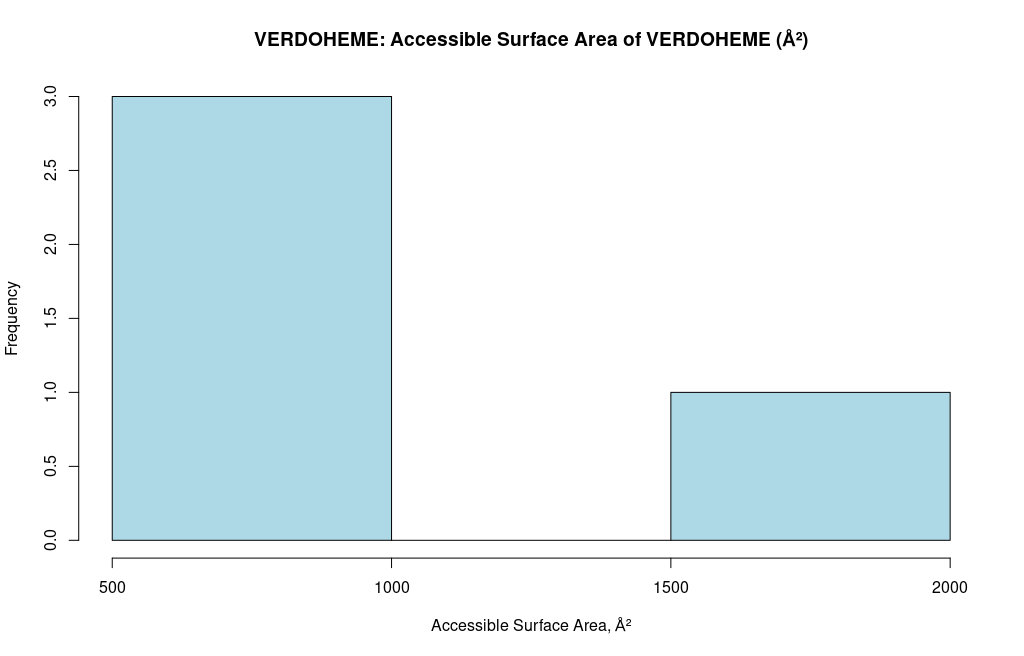
\includegraphics[width=\linewidth]{7A/VERDOHEME_ligandAccSA}
	\end{figure}

\section{Ligand Excluded Surface Area}
	\begin{figure}
		\caption{HEM Ligand Excluded Surface Area}
		\label{figs:HEM_ligandExcSA}
		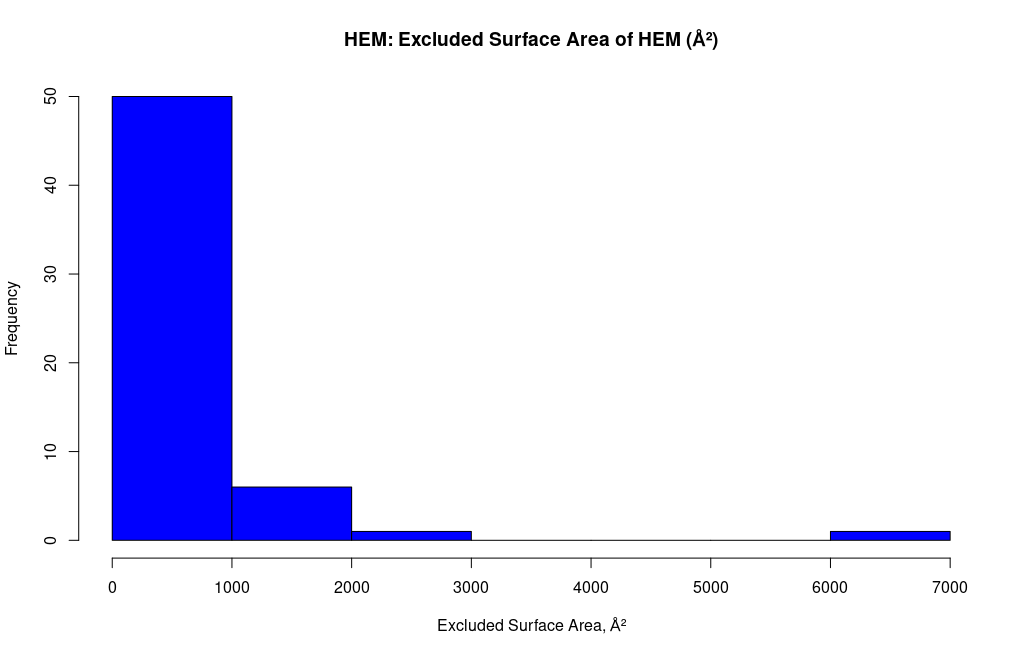
\includegraphics[width=\linewidth]{7A/HEM_ligandExcSA}
	\end{figure}
	
	\begin{figure}
		\caption{HEC Ligand Excluded Surface Area}
		\label{figs:HEC_ligandExcSA}
		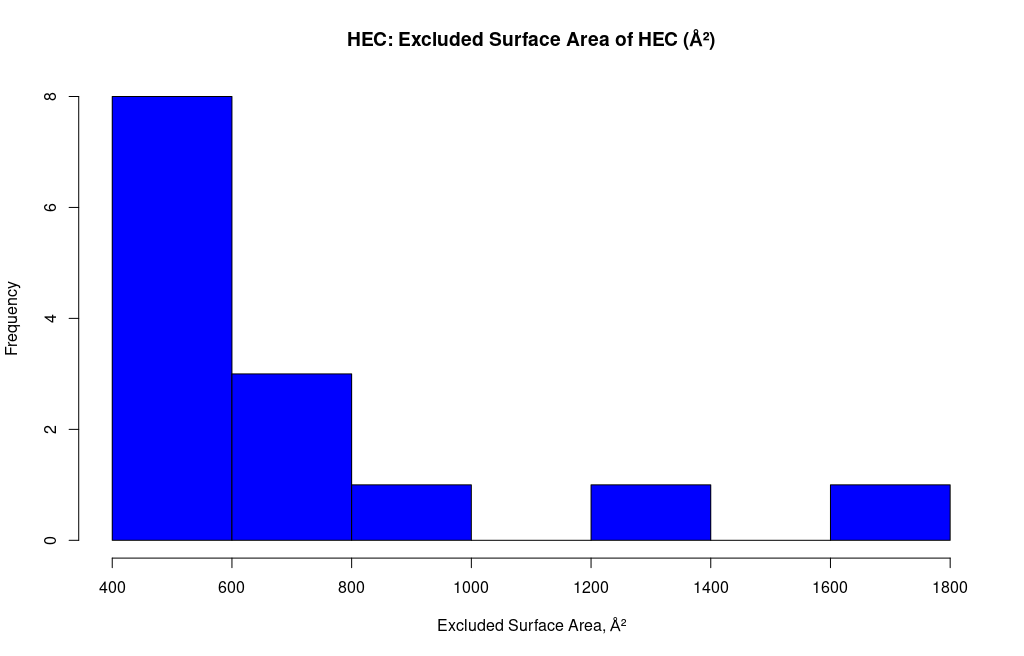
\includegraphics[width=\linewidth]{7A/HEC_ligandExcSA}
	\end{figure}

	\begin{figure}
		\caption{SRM Ligand Excluded Surface Area}
		\label{figs:SRM_ligandExcSA}
		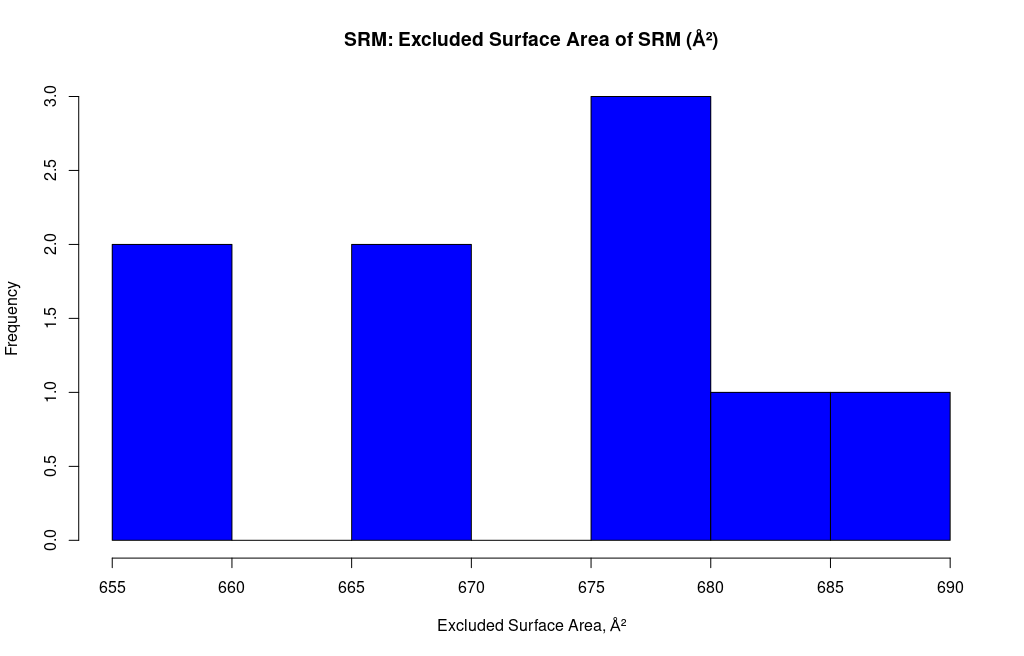
\includegraphics[width=\linewidth]{7A/SRM_ligandExcSA}
	\end{figure}

	\begin{figure}
		\caption{VERDOHEME Ligand Excluded Surface Area}
		\label{figs:VERDOHEME_ligandExcSA}
		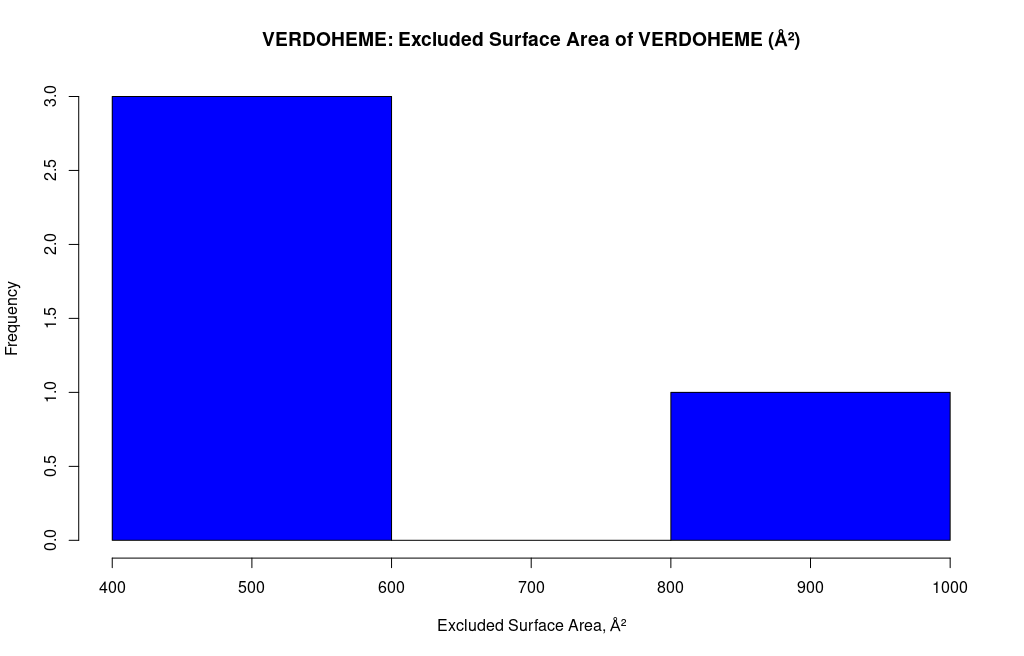
\includegraphics[width=\linewidth]{7A/VERDOHEME_ligandExcSA}
	\end{figure}

\section{Planar Angles}
	\begin{figure}
		\caption{HEM Planar Angles}
		\label{figs:HEM_planarAngles}
		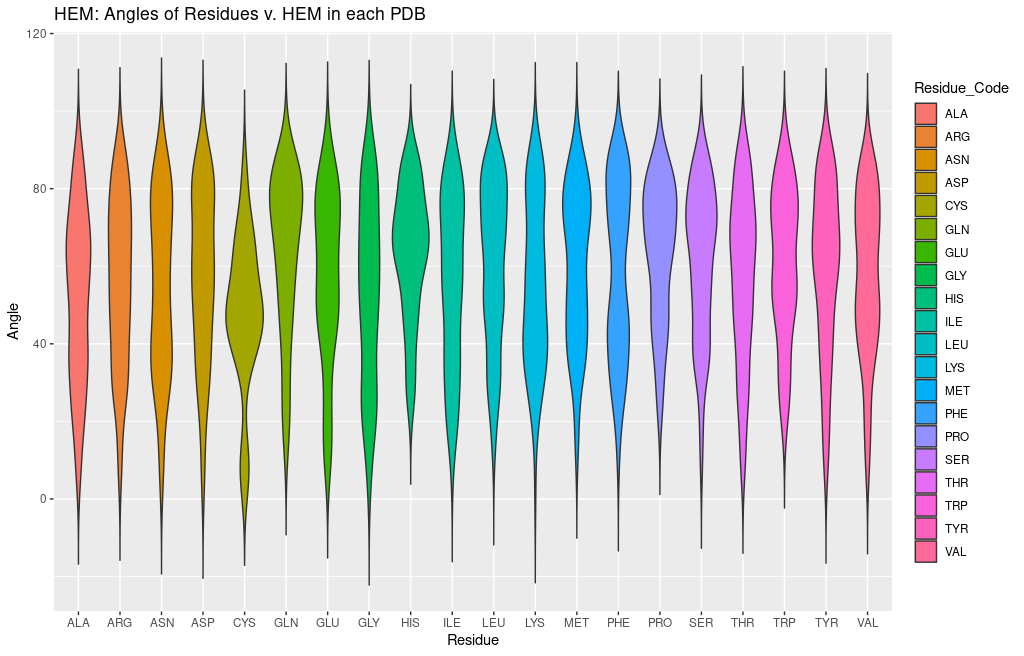
\includegraphics[width=\linewidth]{7A/HEM_planarAngles}
	\end{figure}
	
	\begin{figure}
		\caption{HEC Planar Angles}
		\label{figs:HEC_planarAngles}
		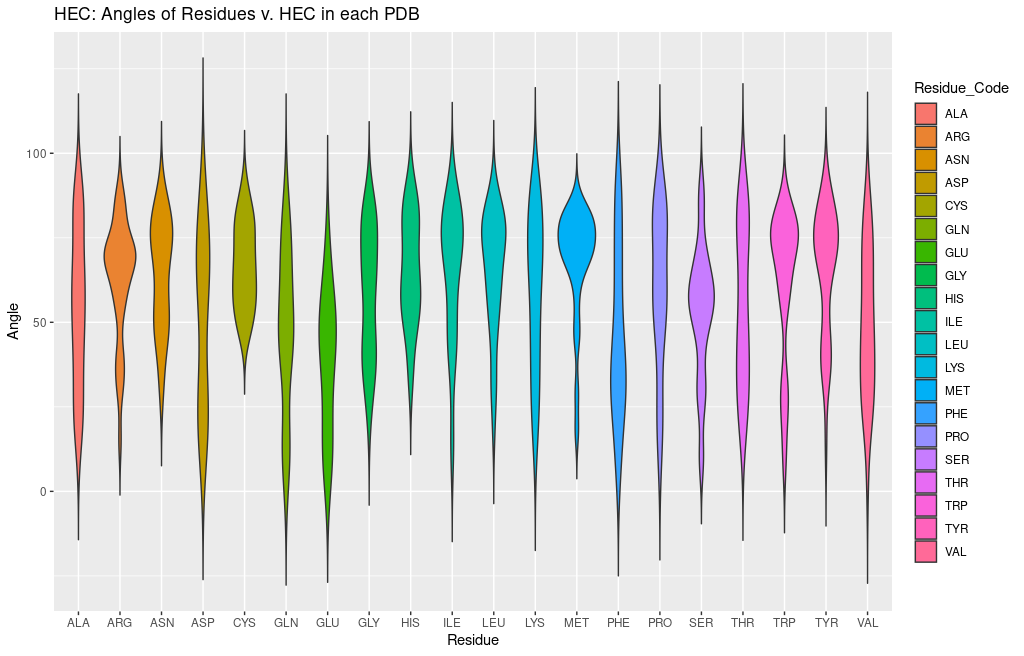
\includegraphics[width=\linewidth]{7A/HEC_planarAngles}
	\end{figure}
	
	\begin{figure}
		\caption{SRM Planar Angles}
		\label{figs:SRM_planarAngles}
		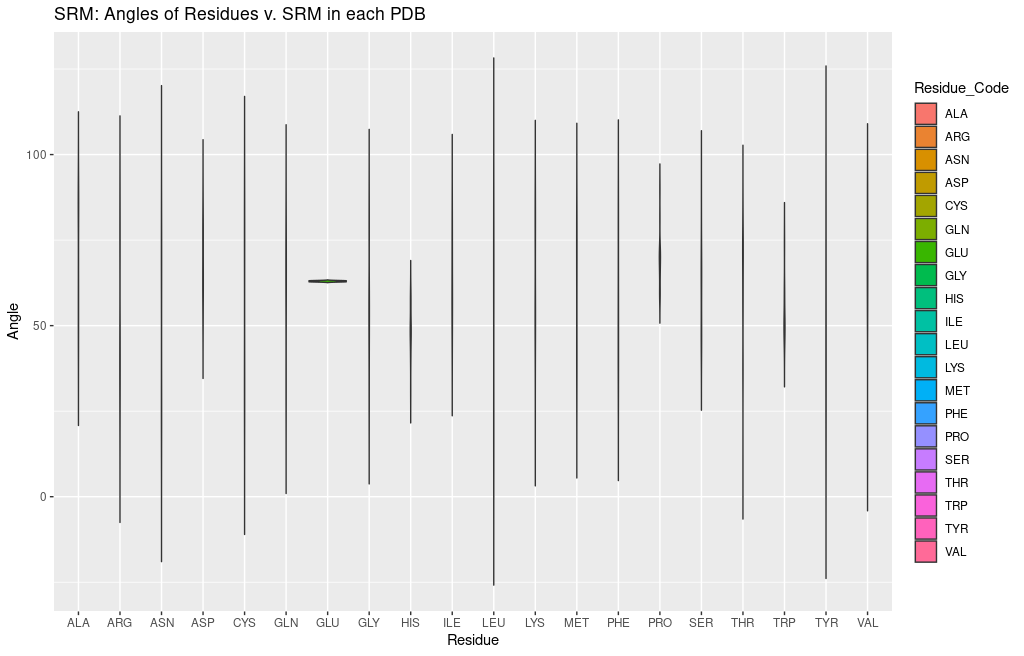
\includegraphics[width=\linewidth]{7A/SRM_planarAngles}
	\end{figure}
	
	\begin{figure}
		\caption{VERDOHEME Planar Angles}
		\label{figs:VERDOHEME_planarAngles}
		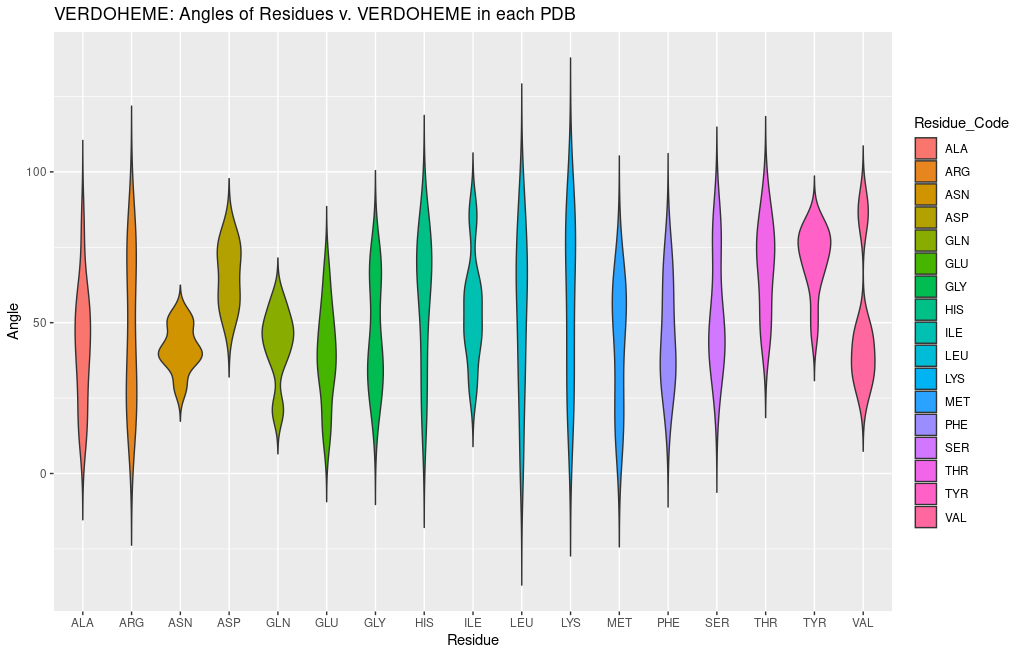
\includegraphics[width=\linewidth]{7A/VERDOHEME_planarAngles}
	\end{figure}
	
\section{Pocket Accessible Surface Area}
	\begin{figure}
		\caption{HEM Pocket Accessible Surface Area}
		\label{figs:HEM_pocketAccSA}
		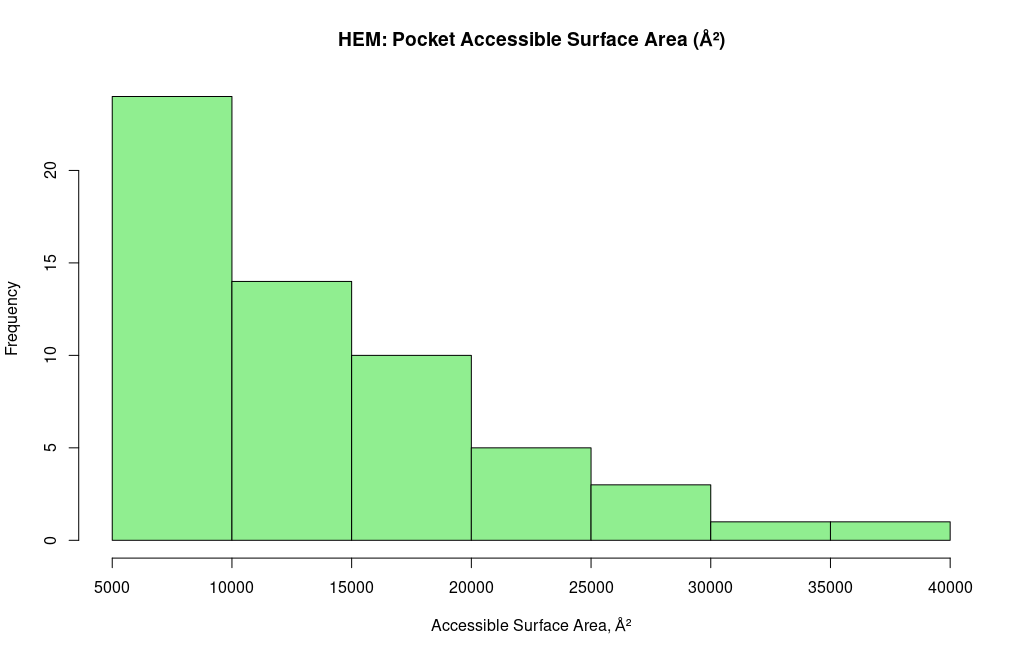
\includegraphics[width=\linewidth]{7A/HEM_pocketAccSA}
	\end{figure}

	\begin{figure}
		\caption{HEC Pocket Accessible Surface Area}
		\label{figs:HEC_pocketAccSA}
		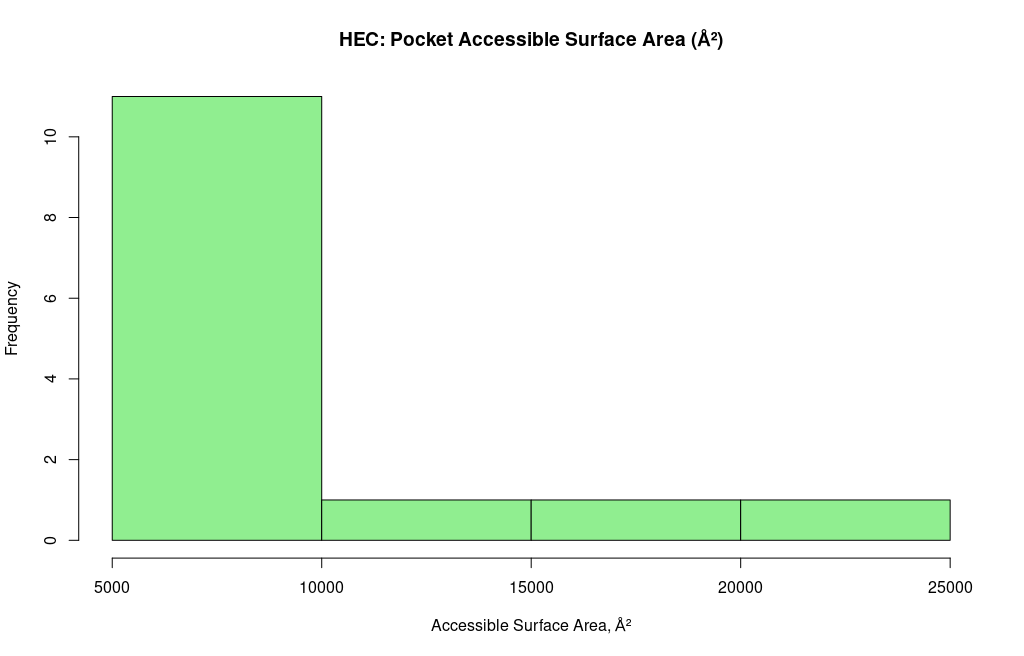
\includegraphics[width=\linewidth]{7A/HEC_pocketAccSA}
	\end{figure}

	\begin{figure}
		\caption{SRM Pocket Accessible Surface Area}
		\label{figs:SRM_pocketAccSA}
		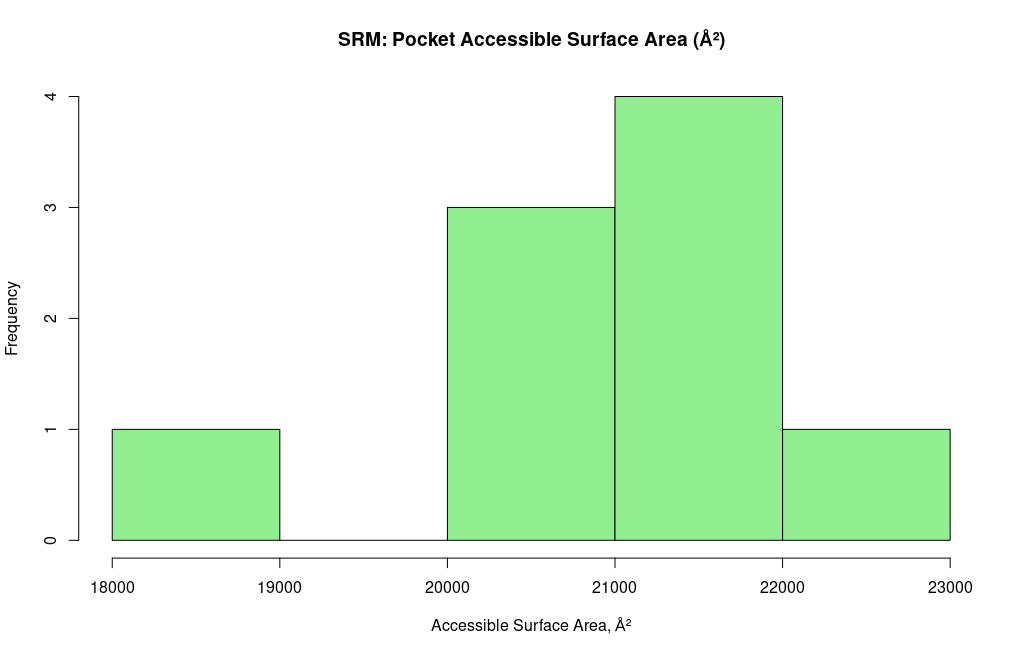
\includegraphics[width=\linewidth]{7A/SRM_pocketAccSA}
	\end{figure}

	\begin{figure}
		\caption{VERDOHEME Pocket Accessible Surface Area}
		\label{figs:VERDOHEME_pocketAccSA}
		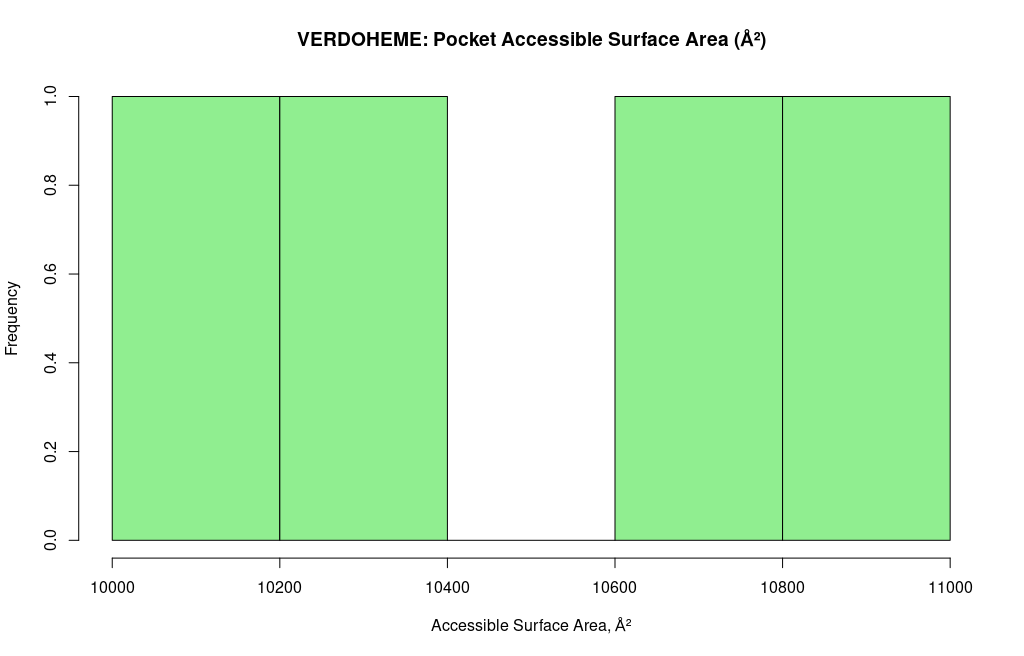
\includegraphics[width=\linewidth]{7A/VERDOHEME_pocketAccSA}
	\end{figure}

\section{Pocket Excluded Surface Area}
	\begin{figure}
		\caption{HEM Pocket Excluded Surface Area}
		\label{figs:HEM_pocketExcSA}
		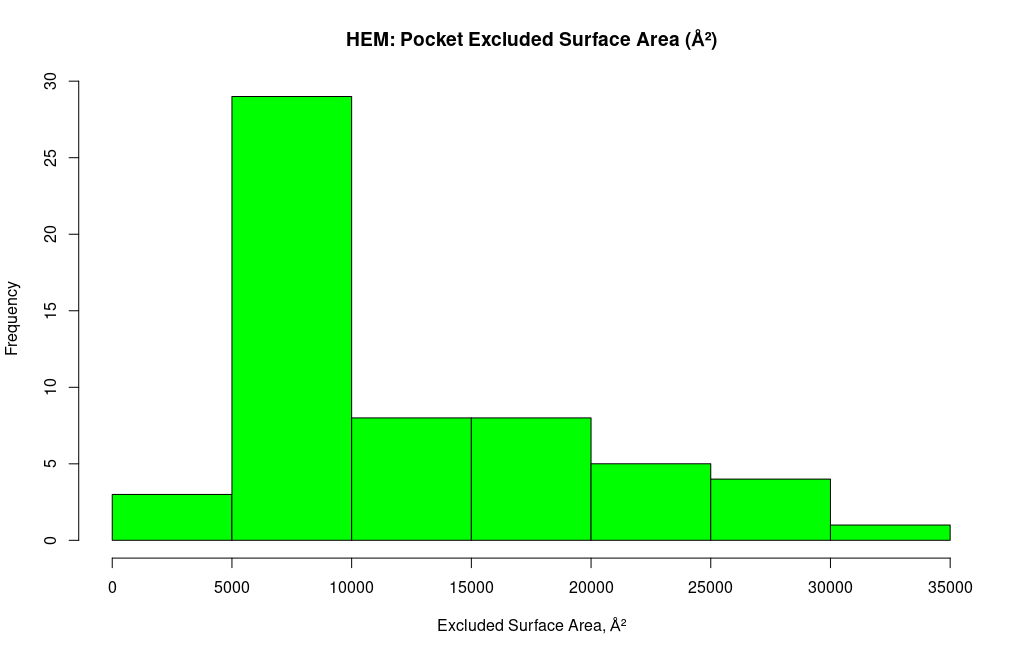
\includegraphics[width=\linewidth]{7A/HEM_pocketExcSA}
	\end{figure}

	\begin{figure}
		\caption{HEC Pocket Excluded Surface Area}
		\label{figs:HEC_pocketExcSA}
		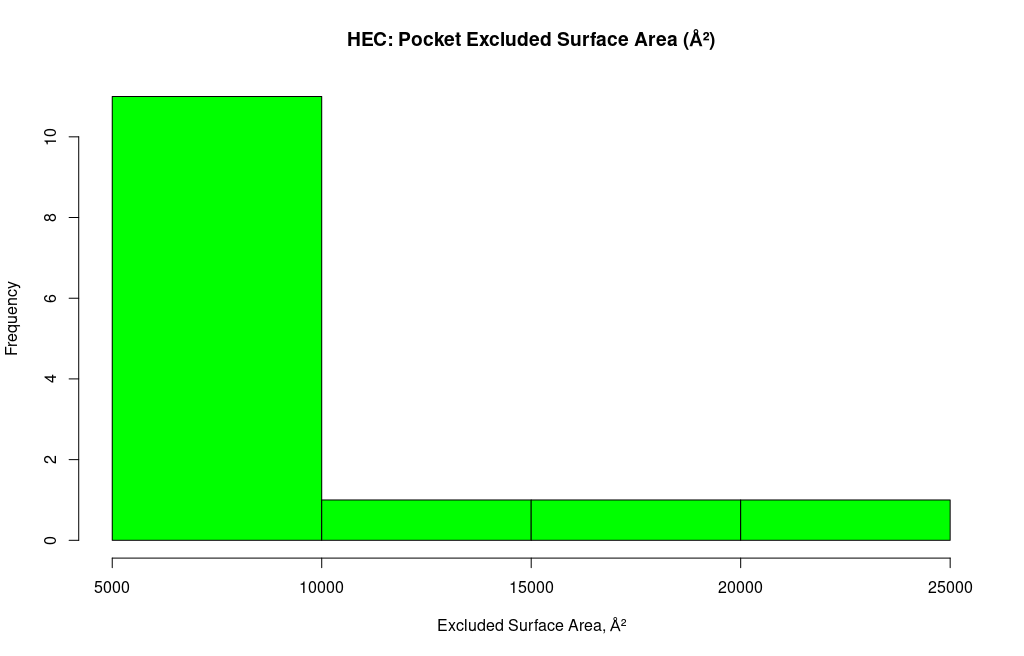
\includegraphics[width=\linewidth]{7A/HEC_pocketExcSA}
	\end{figure}
	
	\begin{figure}
		\caption{SRM Pocket Excluded Surface Area}
		\label{figs:SRM_pocketExcSA}
		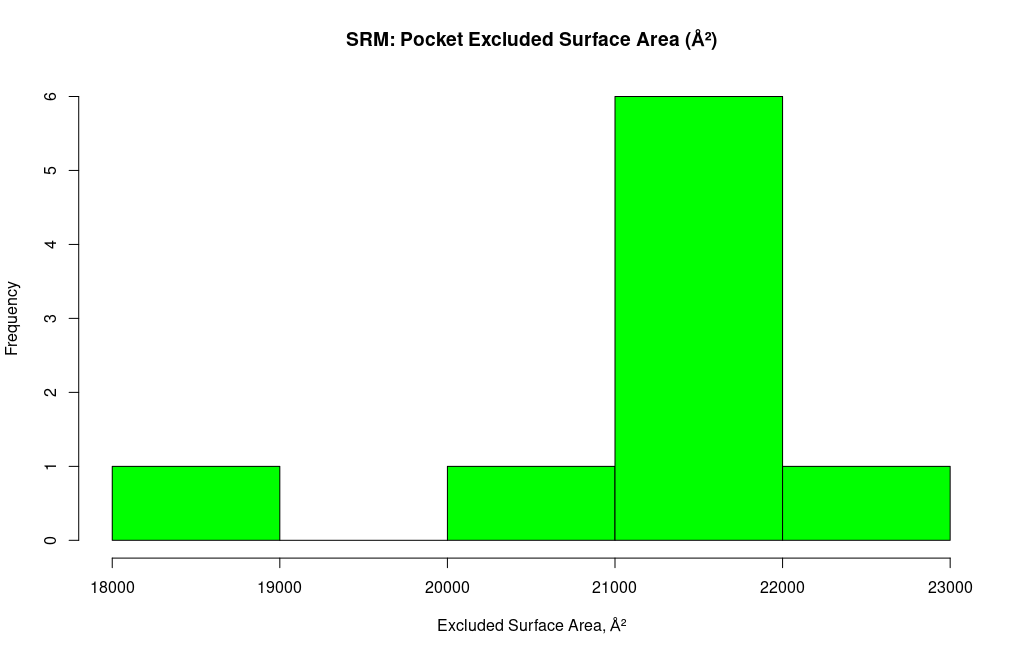
\includegraphics[width=\linewidth]{7A/SRM_pocketExcSA}
	\end{figure}
	
	\begin{figure}
		\caption{VERODHEME Pocket Excluded Surface Area}
		\label{figs:VERDOHEME_pocketExcSA}
		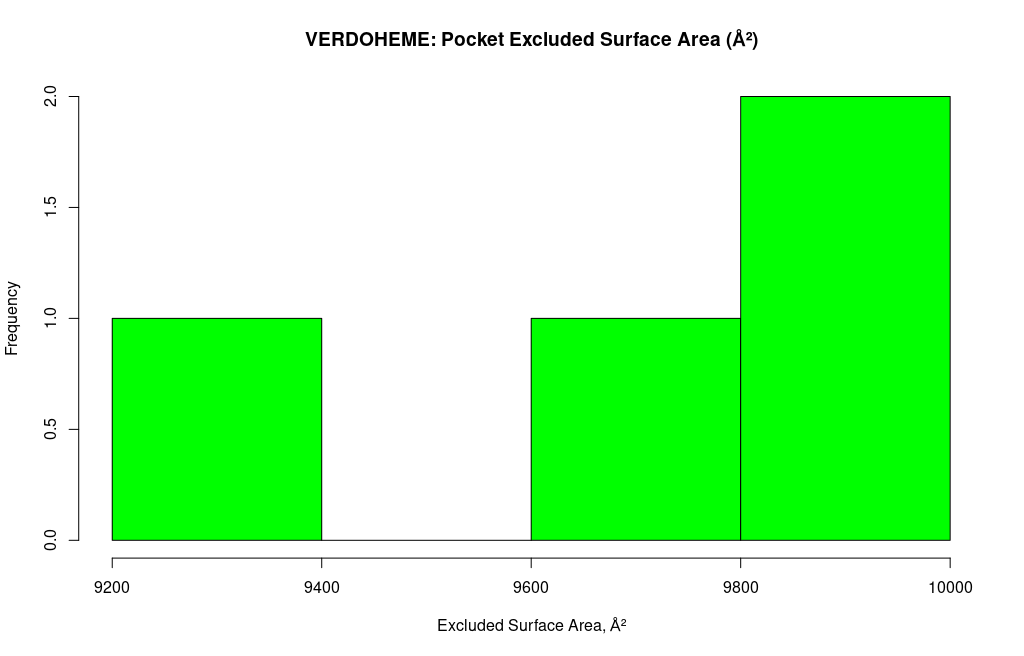
\includegraphics[width=\linewidth]{7A/VERDOHEME_pocketExcSA}
	\end{figure}
	
\section{Volume}
	\begin{figure}
		\caption{HEM Pocket Volume}
		\label{figs:HEM_volume}
		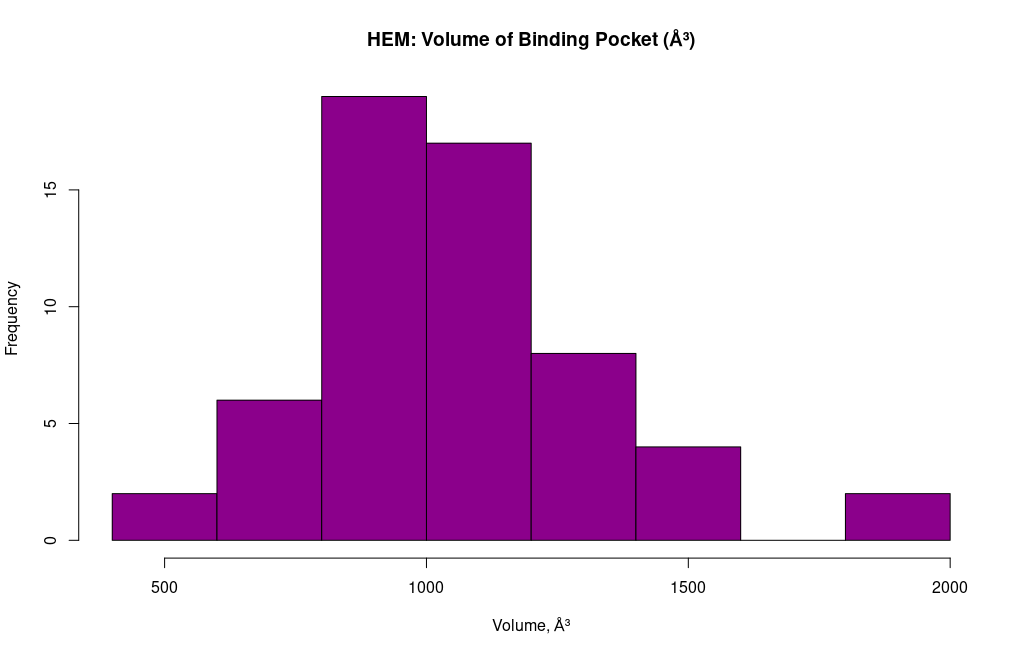
\includegraphics[width=\linewidth]{7A/HEM_volume}
	\end{figure}

	
	\begin{figure}
		\caption{HEC Pocket Volume}
		\label{figs:HEC_volume}
		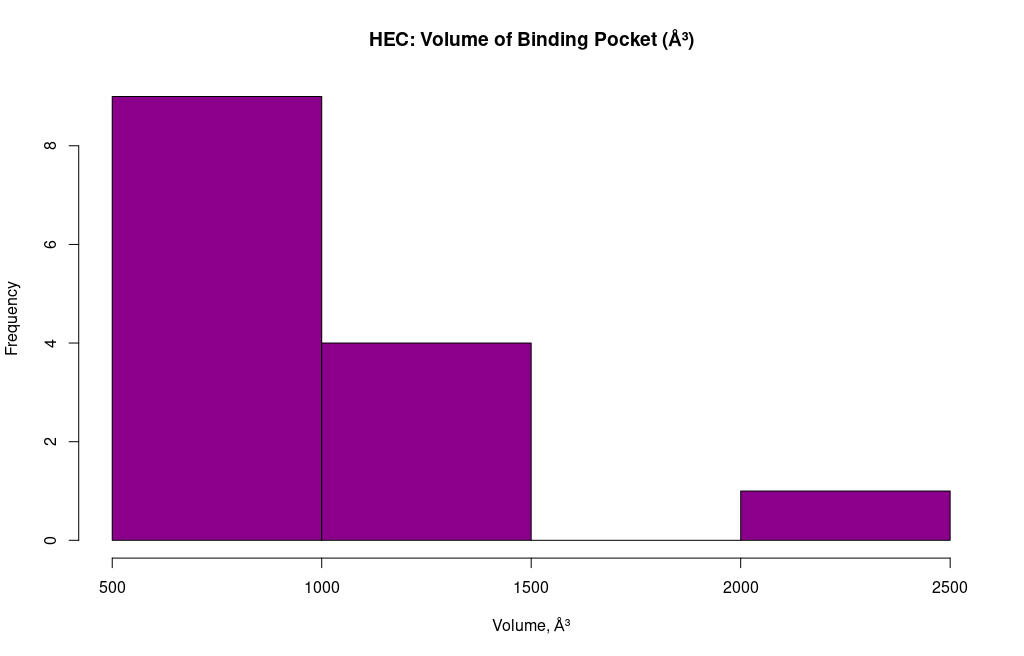
\includegraphics[width=\linewidth]{7A/HEC_volume}
	\end{figure}
	
	
	\begin{figure}
		\caption{SRM Pocket Volume}
		\label{figs:SRM_volume}
		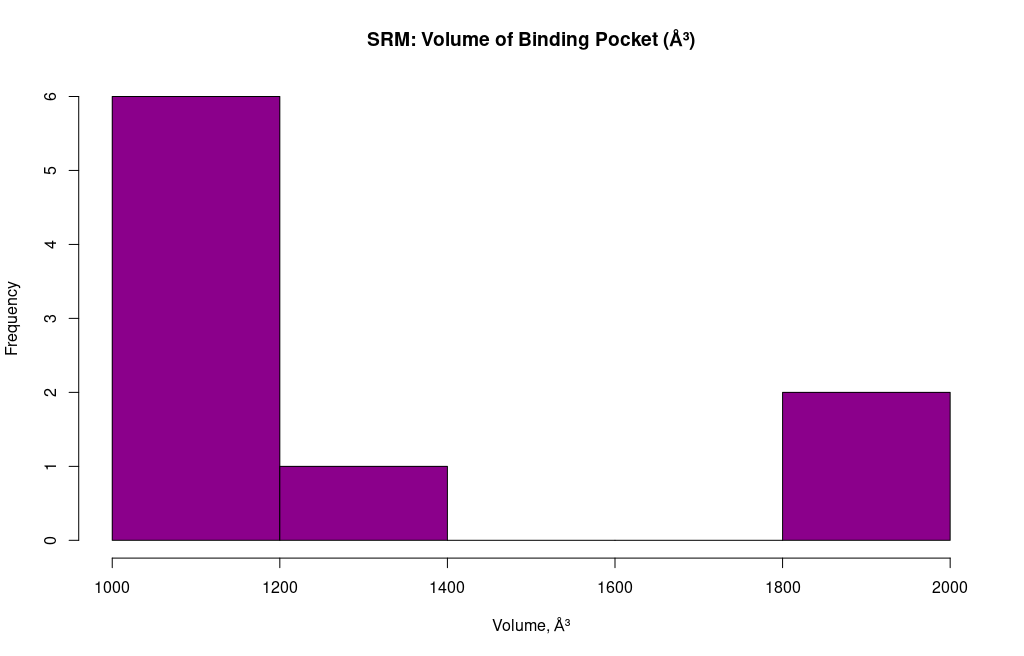
\includegraphics[width=\linewidth]{7A/SRM_volume}
	\end{figure}
	
	
	\begin{figure}
		\caption{VERDOHEME Pocket Volume}
		\label{figs:VERDOHEME_volume}
		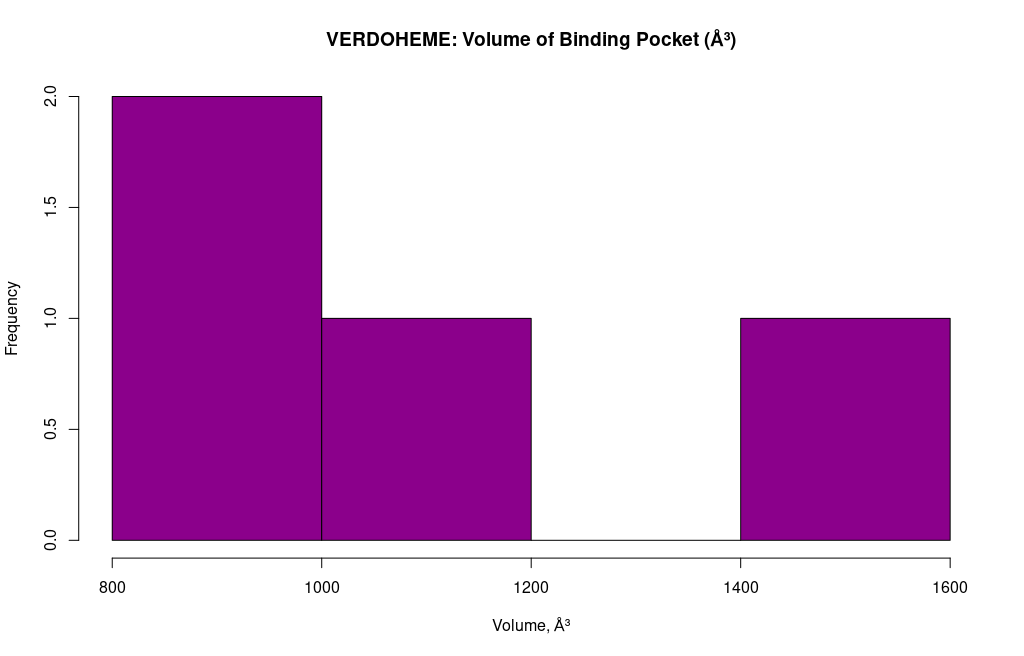
\includegraphics[width=\linewidth]{7A/VERDOHEME_volume}
	\end{figure}
	
	% attempt below to have like a four-way square of stuff going on, but it gets pretty tiny... and probs not necessary

% belows prevent latex from adding whitespace automatically

%\begin{figure}%
%	\centering
%	\subfloat[\centering num1]{{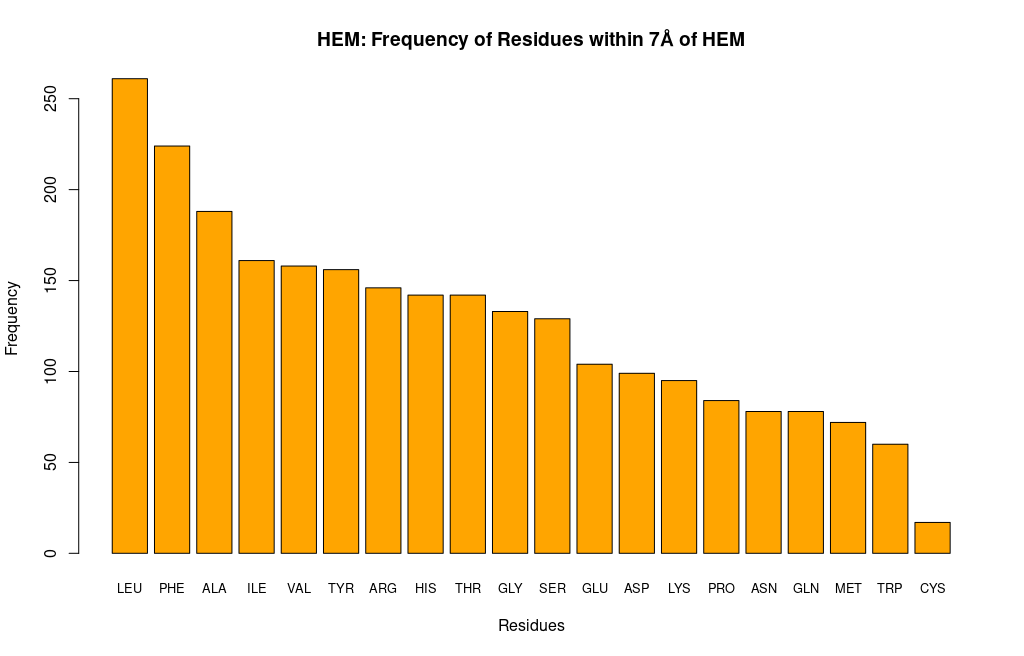
\includegraphics[width=5cm]{7A/HEM_aaFreq}}}%
%	\qquad
%	\subfloat[\centering num2]{{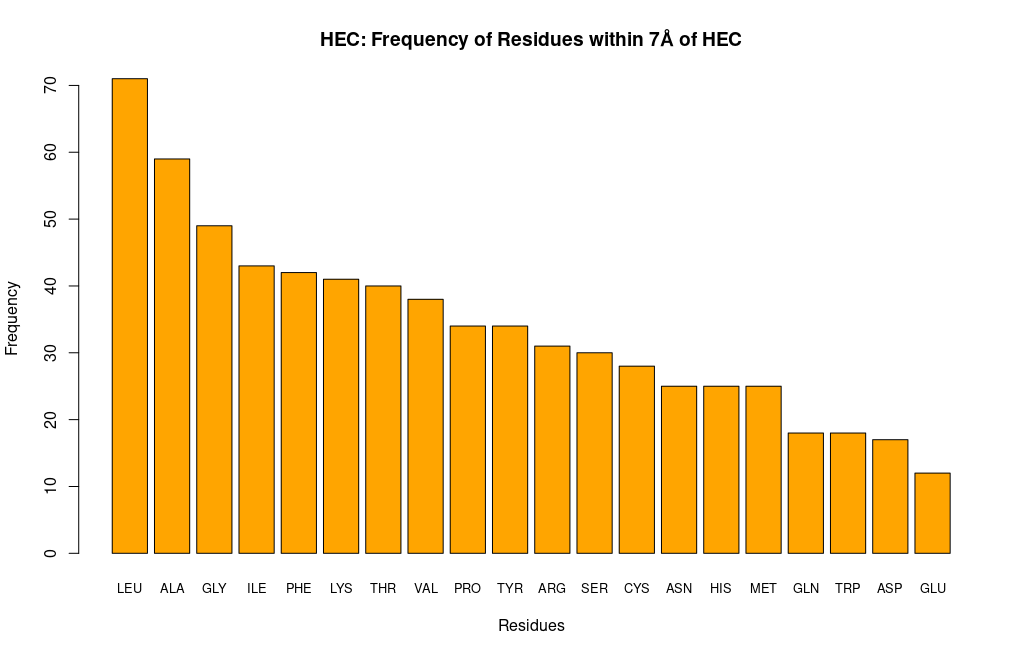
\includegraphics[width=1.0\textwidth]{7A/HEC_aaFreq}}}%
%	\caption{These are two shits}%
%	label{fig:allAAFreq}%
%\end{figure}
			
		\chapter{Tables}
			\section{AA Frequency}
	%so let's input them all here! then just include this for aaFreqTables
	%figures for aa will require similar document but just calling figures
	
	\begin{table}
		\caption{HEM AA freq}
		\label{tbl:HEM_aaFreq}
		\centering
		\begin{tabular}{lr}
			\toprule
			Residue & Freq\\
			\midrule
			\cellcolor{gray!6}{LEU} & \cellcolor{gray!6}{261}\\
			PHE & 224\\
			\cellcolor{gray!6}{ALA} & \cellcolor{gray!6}{188}\\
			ILE & 161\\
			\cellcolor{gray!6}{VAL} & \cellcolor{gray!6}{158}\\
			\addlinespace
			TYR & 156\\
			\cellcolor{gray!6}{ARG} & \cellcolor{gray!6}{146}\\
			HIS & 142\\
			\cellcolor{gray!6}{THR} & \cellcolor{gray!6}{142}\\
			GLY & 133\\
			\addlinespace
			\cellcolor{gray!6}{SER} & \cellcolor{gray!6}{129}\\
			GLU & 104\\
			\cellcolor{gray!6}{ASP} & \cellcolor{gray!6}{99}\\
			LYS & 95\\
			\cellcolor{gray!6}{PRO} & \cellcolor{gray!6}{84}\\
			\addlinespace
			ASN & 78\\
			\cellcolor{gray!6}{GLN} & \cellcolor{gray!6}{78}\\
			MET & 72\\
			\cellcolor{gray!6}{TRP} & \cellcolor{gray!6}{60}\\
			CYS & 17\\
			\bottomrule
		\end{tabular}
	\end{table}

	
	\begin{table}
		\caption{HEC AA Freq}
		\label{tbl:HEC_aaFreq}
		\centering
		\begin{tabular}{lr}
			\toprule
			Residue & Freq\\
			\midrule
			\cellcolor{gray!6}{LEU} & \cellcolor{gray!6}{71}\\
			ALA & 59\\
			\cellcolor{gray!6}{GLY} & \cellcolor{gray!6}{49}\\
			ILE & 43\\
			\cellcolor{gray!6}{PHE} & \cellcolor{gray!6}{42}\\
			\addlinespace
			LYS & 41\\
			\cellcolor{gray!6}{THR} & \cellcolor{gray!6}{40}\\
			VAL & 38\\
			\cellcolor{gray!6}{PRO} & \cellcolor{gray!6}{34}\\
			TYR & 34\\
			\addlinespace
			\cellcolor{gray!6}{ARG} & \cellcolor{gray!6}{31}\\
			SER & 30\\
			\cellcolor{gray!6}{CYS} & \cellcolor{gray!6}{28}\\
			ASN & 25\\
			\cellcolor{gray!6}{HIS} & \cellcolor{gray!6}{25}\\
			\addlinespace
			MET & 25\\
			\cellcolor{gray!6}{GLN} & \cellcolor{gray!6}{18}\\
			TRP & 18\\
			\cellcolor{gray!6}{ASP} & \cellcolor{gray!6}{17}\\
			GLU & 12\\
			\bottomrule
		\end{tabular}
	\end{table}

	\begin{table}
		\caption{SRM AA Freq}
		\label{tbl:SRM_aaFreq}
		\centering
		\begin{tabular}{lr}
			\toprule
			Residue & Freq\\
			\midrule
			\cellcolor{gray!6}{ARG} & \cellcolor{gray!6}{83}\\
			GLN & 51\\
			\cellcolor{gray!6}{CYS} & \cellcolor{gray!6}{43}\\
			LYS & 42\\
			\cellcolor{gray!6}{THR} & \cellcolor{gray!6}{40}\\
			\addlinespace
			ASN & 39\\
			\cellcolor{gray!6}{GLY} & \cellcolor{gray!6}{37}\\
			ALA & 35\\
			\cellcolor{gray!6}{PHE} & \cellcolor{gray!6}{31}\\
			VAL & 31\\
			\addlinespace
			\cellcolor{gray!6}{ASP} & \cellcolor{gray!6}{30}\\
			LEU & 20\\
			\cellcolor{gray!6}{SER} & \cellcolor{gray!6}{20}\\
			MET & 18\\
			\cellcolor{gray!6}{ILE} & \cellcolor{gray!6}{17}\\
			\addlinespace
			PRO & 17\\
			\cellcolor{gray!6}{HIS} & \cellcolor{gray!6}{15}\\
			TRP & 10\\
			\cellcolor{gray!6}{TYR} & \cellcolor{gray!6}{6}\\
			GLU & 2\\
			\bottomrule
		\end{tabular}
	\end{table}

	\begin{table}
		\caption{VERDOHEME AA Freq}
		\label{tbl:VERDOHEME_aaFreq}
		\centering
		\begin{tabular}{lr}
			\toprule
			Residue & Freq\\
			\midrule
			\cellcolor{gray!6}{LEU} & \cellcolor{gray!6}{16}\\
			ALA & 13\\
			\cellcolor{gray!6}{TYR} & \cellcolor{gray!6}{13}\\
			ARG & 11\\
			\cellcolor{gray!6}{GLY} & \cellcolor{gray!6}{11}\\
			\addlinespace
			PHE & 11\\
			\cellcolor{gray!6}{GLU} & \cellcolor{gray!6}{10}\\
			SER & 10\\
			\cellcolor{gray!6}{VAL} & \cellcolor{gray!6}{9}\\
			LYS & 8\\
			\addlinespace
			\cellcolor{gray!6}{ASN} & \cellcolor{gray!6}{7}\\
			HIS & 7\\
			\cellcolor{gray!6}{MET} & \cellcolor{gray!6}{7}\\
			THR & 7\\
			\cellcolor{gray!6}{GLN} & \cellcolor{gray!6}{6}\\
			\addlinespace
			ILE & 6\\
			\cellcolor{gray!6}{ASP} & \cellcolor{gray!6}{4}\\
			\bottomrule
		\end{tabular}
	\end{table}

\section{CACBFe Data}
	\begin{table}
		\caption{HEM CACBFe Data}
		\label{tbl:HEM_cab}
		\centering
		\begin{tabular}{lrlr}
			\toprule
			PDB\_ID & Residue\_Number & Residue\_Code & Angle\\
			\midrule
			\cellcolor{gray!6}{1B2V} & \cellcolor{gray!6}{137} & \cellcolor{gray!6}{TYR} & \cellcolor{gray!6}{107.0750}\\
			1B2V & 140 & MET & 173.7920\\
			\cellcolor{gray!6}{1B2V} & \cellcolor{gray!6}{32} & \cellcolor{gray!6}{HIS} & \cellcolor{gray!6}{116.3150}\\
			1B2V & 37 & VAL & 150.5390\\
			\cellcolor{gray!6}{1B2V} & \cellcolor{gray!6}{41} & \cellcolor{gray!6}{ASN} & \cellcolor{gray!6}{79.4068}\\
			\addlinespace
			1B2V & 42 & SER & 82.8367\\
			\cellcolor{gray!6}{1B2V} & \cellcolor{gray!6}{75} & \cellcolor{gray!6}{TYR} & \cellcolor{gray!6}{132.4540}\\
			1B2V & 77 & LEU & 57.1497\\
			\cellcolor{gray!6}{1B2V} & \cellcolor{gray!6}{83} & \cellcolor{gray!6}{HIS} & \cellcolor{gray!6}{102.9160}\\
			1B2V & 84 & THR & 18.8827\\
			\addlinespace
			\cellcolor{gray!6}{1B5M} & \cellcolor{gray!6}{35} & \cellcolor{gray!6}{PHE} & \cellcolor{gray!6}{126.8820}\\
			1B5M & 39 & HIS & 101.8130\\
			\cellcolor{gray!6}{1B5M} & \cellcolor{gray!6}{40} & \cellcolor{gray!6}{PRO} & \cellcolor{gray!6}{84.9302}\\
			1B5M & 45 & VAL & 132.2220\\
			\cellcolor{gray!6}{1B5M} & \cellcolor{gray!6}{46} & \cellcolor{gray!6}{LEU} & \cellcolor{gray!6}{104.5310}\\
			\addlinespace
			1B5M & 58 & PHE & 85.0021\\
			\cellcolor{gray!6}{1B5M} & \cellcolor{gray!6}{61} & \cellcolor{gray!6}{VAL} & \cellcolor{gray!6}{142.4900}\\
			1B5M & 63 & HIS & 125.8380\\
			\cellcolor{gray!6}{1B5M} & \cellcolor{gray!6}{67} & \cellcolor{gray!6}{ALA} & \cellcolor{gray!6}{143.9450}\\
			1DK0 & 137 & TYR & 107.9930\\
			\addlinespace
			\cellcolor{gray!6}{1DK0} & \cellcolor{gray!6}{140} & \cellcolor{gray!6}{MET} & \cellcolor{gray!6}{173.4760}\\
			1DK0 & 32 & HIS & 116.4470\\
			\cellcolor{gray!6}{1DK0} & \cellcolor{gray!6}{33} & \cellcolor{gray!6}{THR} & \cellcolor{gray!6}{13.7171}\\
			1DK0 & 37 & VAL & 154.2260\\
			\cellcolor{gray!6}{1DK0} & \cellcolor{gray!6}{41} & \cellcolor{gray!6}{ASN} & \cellcolor{gray!6}{80.6960}\\
			\addlinespace
			1DK0 & 42 & SER & 80.4760\\
			\cellcolor{gray!6}{1DK0} & \cellcolor{gray!6}{75} & \cellcolor{gray!6}{TYR} & \cellcolor{gray!6}{131.4420}\\
			1DK0 & 77 & LEU & 58.1793\\
			\cellcolor{gray!6}{1DK0} & \cellcolor{gray!6}{83} & \cellcolor{gray!6}{HIS} & \cellcolor{gray!6}{102.7520}\\
			1DK0 & 84 & THR & 19.3165\\
			\addlinespace
			\cellcolor{gray!6}{1DKH} & \cellcolor{gray!6}{137} & \cellcolor{gray!6}{TYR} & \cellcolor{gray!6}{103.9420}\\
			1DKH & 140 & MET & 172.2070\\
			\cellcolor{gray!6}{1DKH} & \cellcolor{gray!6}{32} & \cellcolor{gray!6}{HIS} & \cellcolor{gray!6}{121.3750}\\
			1DKH & 37 & VAL & 149.8520\\
			\cellcolor{gray!6}{1DKH} & \cellcolor{gray!6}{42} & \cellcolor{gray!6}{SER} & \cellcolor{gray!6}{32.8371}\\
			\addlinespace
			1DKH & 75 & TYR & 125.4210\\
			\cellcolor{gray!6}{1DKH} & \cellcolor{gray!6}{77} & \cellcolor{gray!6}{LEU} & \cellcolor{gray!6}{66.1552}\\
			1DKH & 83 & HIS & 122.9600\\
			\cellcolor{gray!6}{1DKH} & \cellcolor{gray!6}{84} & \cellcolor{gray!6}{THR} & \cellcolor{gray!6}{31.3703}\\
			1ICC & 35 & PHE & 121.2740\\
			\addlinespace
			\cellcolor{gray!6}{1ICC} & \cellcolor{gray!6}{39} & \cellcolor{gray!6}{HIS} & \cellcolor{gray!6}{101.5070}\\
			1ICC & 40 & PRO & 84.5709\\
			\cellcolor{gray!6}{1ICC} & \cellcolor{gray!6}{45} & \cellcolor{gray!6}{VAL} & \cellcolor{gray!6}{128.6010}\\
			1ICC & 46 & LEU & 99.3266\\
			\cellcolor{gray!6}{1ICC} & \cellcolor{gray!6}{58} & \cellcolor{gray!6}{PHE} & \cellcolor{gray!6}{70.5320}\\
			\addlinespace
			1ICC & 61 & VAL & 157.5600\\
			\cellcolor{gray!6}{1ICC} & \cellcolor{gray!6}{63} & \cellcolor{gray!6}{HIS} & \cellcolor{gray!6}{114.1290}\\
			1ICC & 67 & ALA & 131.3420\\
			\cellcolor{gray!6}{1IPH} & \cellcolor{gray!6}{127} & \cellcolor{gray!6}{VAL} & \cellcolor{gray!6}{129.5510}\\
			1IPH & 128 & HIS & 129.2180\\
			\addlinespace
			\cellcolor{gray!6}{1IPH} & \cellcolor{gray!6}{199} & \cellcolor{gray!6}{VAL} & \cellcolor{gray!6}{124.0950}\\
			1IPH & 201 & ASN & 101.2860\\
			\cellcolor{gray!6}{1IPH} & \cellcolor{gray!6}{206} & \cellcolor{gray!6}{PHE} & \cellcolor{gray!6}{134.5530}\\
			1IPH & 214 & PHE & 138.4550\\
			\cellcolor{gray!6}{1IPH} & \cellcolor{gray!6}{393} & \cellcolor{gray!6}{PRO} & \cellcolor{gray!6}{126.7810}\\
			\addlinespace
			1IPH & 411 & ARG & 108.2630\\
			\cellcolor{gray!6}{1IPH} & \cellcolor{gray!6}{414} & \cellcolor{gray!6}{SER} & \cellcolor{gray!6}{141.7910}\\
			1IPH & 415 & TYR & 114.2710\\
			\cellcolor{gray!6}{1N45} & \cellcolor{gray!6}{135} & \cellcolor{gray!6}{THR} & \cellcolor{gray!6}{60.4070}\\
			1N45 & 138 & LEU & 68.2659\\
			\addlinespace
			\cellcolor{gray!6}{1N45} & \cellcolor{gray!6}{140} & \cellcolor{gray!6}{ASP} & \cellcolor{gray!6}{35.7360}\\
			1N45 & 142 & SER & 110.0660\\
			\cellcolor{gray!6}{1N45} & \cellcolor{gray!6}{147} & \cellcolor{gray!6}{LEU} & \cellcolor{gray!6}{123.9670}\\
			1N45 & 207 & PHE & 104.6170\\
			\cellcolor{gray!6}{1N45} & \cellcolor{gray!6}{25} & \cellcolor{gray!6}{HIS} & \cellcolor{gray!6}{112.7600}\\
			\addlinespace
			1N45 & 28 & ALA & 133.1800\\
			\cellcolor{gray!6}{1N45} & \cellcolor{gray!6}{29} & \cellcolor{gray!6}{GLU} & \cellcolor{gray!6}{93.8698}\\
			1P3T & 113 & CYS & 62.2220\\
			\cellcolor{gray!6}{1P3T} & \cellcolor{gray!6}{117} & \cellcolor{gray!6}{SER} & \cellcolor{gray!6}{57.1608}\\
			1P3T & 118 & ASN & 26.9658\\
			\addlinespace
			\cellcolor{gray!6}{1P3T} & \cellcolor{gray!6}{119} & \cellcolor{gray!6}{LEU} & \cellcolor{gray!6}{90.3174}\\
			1P3T & 121 & ALA & 48.9641\\
			\cellcolor{gray!6}{1P3T} & \cellcolor{gray!6}{181} & \cellcolor{gray!6}{PHE} & \cellcolor{gray!6}{104.9100}\\
			1P3T & 23 & HIS & 111.7580\\
			\cellcolor{gray!6}{1P3T} & \cellcolor{gray!6}{26} & \cellcolor{gray!6}{VAL} & \cellcolor{gray!6}{118.5490}\\
			\addlinespace
			1P3T & 27 & ASP & 103.4810\\
			\cellcolor{gray!6}{1QHU} & \cellcolor{gray!6}{171} & \cellcolor{gray!6}{TRP} & \cellcolor{gray!6}{135.3190}\\
			1QHU & 203 & ASP & 76.4671\\
			\cellcolor{gray!6}{1QHU} & \cellcolor{gray!6}{204} & \cellcolor{gray!6}{TYR} & \cellcolor{gray!6}{82.8848}\\
			1QHU & 213 & HIS & 114.5350\\
			\addlinespace
			\cellcolor{gray!6}{1QHU} & \cellcolor{gray!6}{214} & \cellcolor{gray!6}{ARG} & \cellcolor{gray!6}{137.0270}\\
			1QHU & 222 & HIS & 173.7070\\
			\cellcolor{gray!6}{1QHU} & \cellcolor{gray!6}{225} & \cellcolor{gray!6}{GLU} & \cellcolor{gray!6}{167.2860}\\
			1QHU & 265 & HIS & 121.1810\\
			\cellcolor{gray!6}{1QHU} & \cellcolor{gray!6}{266} & \cellcolor{gray!6}{SER} & \cellcolor{gray!6}{59.3970}\\
			\addlinespace
			1QHU & 267 & TRP & 70.5501\\
			\cellcolor{gray!6}{1QJS} & \cellcolor{gray!6}{171} & \cellcolor{gray!6}{TRP} & \cellcolor{gray!6}{138.2760}\\
			1QJS & 203 & ASP & 70.4888\\
			\cellcolor{gray!6}{1QJS} & \cellcolor{gray!6}{204} & \cellcolor{gray!6}{TYR} & \cellcolor{gray!6}{82.0806}\\
			1QJS & 213 & HIS & 122.0930\\
			\addlinespace
			\cellcolor{gray!6}{1QJS} & \cellcolor{gray!6}{214} & \cellcolor{gray!6}{ARG} & \cellcolor{gray!6}{70.2144}\\
			1QJS & 226 & GLU & 155.6740\\
			\cellcolor{gray!6}{1QJS} & \cellcolor{gray!6}{266} & \cellcolor{gray!6}{HIS} & \cellcolor{gray!6}{120.9930}\\
			1QJS & 267 & SER & 71.5751\\
			\cellcolor{gray!6}{1QJS} & \cellcolor{gray!6}{268} & \cellcolor{gray!6}{TRP} & \cellcolor{gray!6}{64.5387}\\
			\addlinespace
			1SI8 & 125 & VAL & 127.3950\\
			\cellcolor{gray!6}{1SI8} & \cellcolor{gray!6}{127} & \cellcolor{gray!6}{ASN} & \cellcolor{gray!6}{103.3680}\\
			1SI8 & 132 & PHE & 138.1490\\
			\cellcolor{gray!6}{1SI8} & \cellcolor{gray!6}{140} & \cellcolor{gray!6}{PHE} & \cellcolor{gray!6}{139.2170}\\
			1SI8 & 315 & PRO & 121.9570\\
			\addlinespace
			\cellcolor{gray!6}{1SI8} & \cellcolor{gray!6}{333} & \cellcolor{gray!6}{ARG} & \cellcolor{gray!6}{116.1170}\\
			1SI8 & 337 & TYR & 101.8400\\
			\cellcolor{gray!6}{1SI8} & \cellcolor{gray!6}{53} & \cellcolor{gray!6}{VAL} & \cellcolor{gray!6}{132.7600}\\
			1SI8 & 54 & HIS & 131.6120\\
			\cellcolor{gray!6}{1SY2} & \cellcolor{gray!6}{121} & \cellcolor{gray!6}{THR} & \cellcolor{gray!6}{142.1010}\\
			\addlinespace
			1SY2 & 123 & LEU & 147.6300\\
			\cellcolor{gray!6}{1SY2} & \cellcolor{gray!6}{133} & \cellcolor{gray!6}{LEU} & \cellcolor{gray!6}{171.7810}\\
			1SY2 & 36 & VAL & 130.3660\\
			\cellcolor{gray!6}{1SY2} & \cellcolor{gray!6}{40} & \cellcolor{gray!6}{TYR} & \cellcolor{gray!6}{145.2220}\\
			1SY2 & 42 & ALA & 148.0360\\
			\addlinespace
			\cellcolor{gray!6}{1SY2} & \cellcolor{gray!6}{57} & \cellcolor{gray!6}{LEU} & \cellcolor{gray!6}{142.4070}\\
			1SY2 & 58 & TYR & 29.9485\\
			\cellcolor{gray!6}{1SY2} & \cellcolor{gray!6}{59} & \cellcolor{gray!6}{HIS} & \cellcolor{gray!6}{126.3700}\\
			1SY2 & 68 & PHE & 105.5040\\
			\cellcolor{gray!6}{1U9U} & \cellcolor{gray!6}{35} & \cellcolor{gray!6}{PHE} & \cellcolor{gray!6}{120.9680}\\
			\addlinespace
			1U9U & 39 & HIS & 102.2750\\
			\cellcolor{gray!6}{1U9U} & \cellcolor{gray!6}{40} & \cellcolor{gray!6}{PRO} & \cellcolor{gray!6}{87.3619}\\
			1U9U & 45 & VAL & 133.1230\\
			\cellcolor{gray!6}{1U9U} & \cellcolor{gray!6}{46} & \cellcolor{gray!6}{LEU} & \cellcolor{gray!6}{99.9911}\\
			1U9U & 58 & TYR & 75.1903\\
			\addlinespace
			\cellcolor{gray!6}{1U9U} & \cellcolor{gray!6}{61} & \cellcolor{gray!6}{VAL} & \cellcolor{gray!6}{152.2510}\\
			1U9U & 63 & HIS & 116.0130\\
			\cellcolor{gray!6}{1U9U} & \cellcolor{gray!6}{67} & \cellcolor{gray!6}{ALA} & \cellcolor{gray!6}{136.6100}\\
			1VGI & 135 & THR & 58.3823\\
			\cellcolor{gray!6}{1VGI} & \cellcolor{gray!6}{138} & \cellcolor{gray!6}{LEU} & \cellcolor{gray!6}{81.0454}\\
			\addlinespace
			1VGI & 140 & ASP & 22.5121\\
			\cellcolor{gray!6}{1VGI} & \cellcolor{gray!6}{142} & \cellcolor{gray!6}{SER} & \cellcolor{gray!6}{125.4790}\\
			1VGI & 207 & PHE & 106.2160\\
			\cellcolor{gray!6}{1VGI} & \cellcolor{gray!6}{25} & \cellcolor{gray!6}{HIS} & \cellcolor{gray!6}{113.1630}\\
			1VGI & 29 & GLU & 118.3990\\
			\addlinespace
			\cellcolor{gray!6}{1ZVI} & \cellcolor{gray!6}{409} & \cellcolor{gray!6}{TRP} & \cellcolor{gray!6}{90.9270}\\
			1ZVI & 412 & ALA & 147.8760\\
			\cellcolor{gray!6}{1ZVI} & \cellcolor{gray!6}{414} & \cellcolor{gray!6}{ARG} & \cellcolor{gray!6}{71.6516}\\
			1ZVI & 415 & CYS & 112.7440\\
			\cellcolor{gray!6}{1ZVI} & \cellcolor{gray!6}{416} & \cellcolor{gray!6}{VAL} & \cellcolor{gray!6}{55.0798}\\
			\addlinespace
			1ZVI & 418 & ARG & 69.7795\\
			\cellcolor{gray!6}{1ZVI} & \cellcolor{gray!6}{584} & \cellcolor{gray!6}{PHE} & \cellcolor{gray!6}{116.6380}\\
			1ZVI & 587 & TRP & 40.2585\\
			\cellcolor{gray!6}{1ZVI} & \cellcolor{gray!6}{592} & \cellcolor{gray!6}{GLU} & \cellcolor{gray!6}{140.0500}\\
			2BHJ & 188 & TRP & 95.4808\\
			\addlinespace
			\cellcolor{gray!6}{2BHJ} & \cellcolor{gray!6}{191} & \cellcolor{gray!6}{ALA} & \cellcolor{gray!6}{163.9660}\\
			2BHJ & 193 & ARG & 61.6429\\
			\cellcolor{gray!6}{2BHJ} & \cellcolor{gray!6}{194} & \cellcolor{gray!6}{CYS} & \cellcolor{gray!6}{118.0500}\\
			2BHJ & 195 & ILE & 54.9628\\
			\cellcolor{gray!6}{2BHJ} & \cellcolor{gray!6}{197} & \cellcolor{gray!6}{ARG} & \cellcolor{gray!6}{67.6390}\\
			\addlinespace
			2BHJ & 346 & VAL & 125.1020\\
			\cellcolor{gray!6}{2BHJ} & \cellcolor{gray!6}{363} & \cellcolor{gray!6}{PHE} & \cellcolor{gray!6}{116.4950}\\
			2BHJ & 364 & ASN & 23.4362\\
			\cellcolor{gray!6}{2BHJ} & \cellcolor{gray!6}{366} & \cellcolor{gray!6}{TRP} & \cellcolor{gray!6}{39.6654}\\
			2CJ0 & 103 & PHE & 112.2600\\
			\addlinespace
			\cellcolor{gray!6}{2CJ0} & \cellcolor{gray!6}{183} & \cellcolor{gray!6}{GLU} & \cellcolor{gray!6}{106.0810}\\
			2CJ0 & 186 & PHE & 170.8360\\
			\cellcolor{gray!6}{2CJ0} & \cellcolor{gray!6}{213} & \cellcolor{gray!6}{TRP} & \cellcolor{gray!6}{116.4780}\\
			2CJ0 & 28 & PRO & 76.4322\\
			\cellcolor{gray!6}{2CJ0} & \cellcolor{gray!6}{29} & \cellcolor{gray!6}{CYS} & \cellcolor{gray!6}{117.5660}\\
			\addlinespace
			2CJ0 & 30 & PRO & 65.8824\\
			\cellcolor{gray!6}{2CJ0} & \cellcolor{gray!6}{31} & \cellcolor{gray!6}{ALA} & \cellcolor{gray!6}{114.8710}\\
			2CJ0 & 32 & LEU & 97.6039\\
			\cellcolor{gray!6}{2CJ0} & \cellcolor{gray!6}{57} & \cellcolor{gray!6}{PHE} & \cellcolor{gray!6}{126.1650}\\
			2CJ0 & 71 & ALA & 140.1920\\
			\addlinespace
			\cellcolor{gray!6}{2CN4} & \cellcolor{gray!6}{137} & \cellcolor{gray!6}{TYR} & \cellcolor{gray!6}{102.8860}\\
			2CN4 & 140 & MET & 172.2930\\
			\cellcolor{gray!6}{2CN4} & \cellcolor{gray!6}{55} & \cellcolor{gray!6}{TYR} & \cellcolor{gray!6}{136.9090}\\
			2CN4 & 75 & TYR & 126.9230\\
			\cellcolor{gray!6}{2CN4} & \cellcolor{gray!6}{77} & \cellcolor{gray!6}{LEU} & \cellcolor{gray!6}{53.5337}\\
			\addlinespace
			2CN4 & 83 & HIS & 107.5140\\
			\cellcolor{gray!6}{2CN4} & \cellcolor{gray!6}{84} & \cellcolor{gray!6}{THR} & \cellcolor{gray!6}{19.9645}\\
			2CPO & 103 & PHE & 112.7860\\
			\cellcolor{gray!6}{2CPO} & \cellcolor{gray!6}{183} & \cellcolor{gray!6}{GLU} & \cellcolor{gray!6}{105.9460}\\
			2CPO & 186 & PHE & 173.0070\\
			\addlinespace
			\cellcolor{gray!6}{2CPO} & \cellcolor{gray!6}{28} & \cellcolor{gray!6}{PRO} & \cellcolor{gray!6}{69.8826}\\
			2CPO & 29 & CYS & 118.1890\\
			\cellcolor{gray!6}{2CPO} & \cellcolor{gray!6}{30} & \cellcolor{gray!6}{PRO} & \cellcolor{gray!6}{65.4937}\\
			2CPO & 31 & ALA & 115.0400\\
			\cellcolor{gray!6}{2CPO} & \cellcolor{gray!6}{32} & \cellcolor{gray!6}{LEU} & \cellcolor{gray!6}{99.3621}\\
			\addlinespace
			2CPO & 57 & PHE & 125.6230\\
			\cellcolor{gray!6}{2CPO} & \cellcolor{gray!6}{71} & \cellcolor{gray!6}{ALA} & \cellcolor{gray!6}{137.2830}\\
			2E2Y & 104 & LEU & 87.1682\\
			\cellcolor{gray!6}{2E2Y} & \cellcolor{gray!6}{107} & \cellcolor{gray!6}{ILE} & \cellcolor{gray!6}{171.6940}\\
			2E2Y & 43 & TRP & 95.5213\\
			\addlinespace
			\cellcolor{gray!6}{2E2Y} & \cellcolor{gray!6}{64} & \cellcolor{gray!6}{ASP} & \cellcolor{gray!6}{101.7770}\\
			2E2Y & 67 & THR & 106.0790\\
			\cellcolor{gray!6}{2E2Y} & \cellcolor{gray!6}{68} & \cellcolor{gray!6}{ILE} & \cellcolor{gray!6}{97.7283}\\
			2E2Y & 89 & LEU & 89.7887\\
			\cellcolor{gray!6}{2E2Y} & \cellcolor{gray!6}{92} & \cellcolor{gray!6}{SER} & \cellcolor{gray!6}{115.2050}\\
			\addlinespace
			2E2Y & 93 & HIS & 114.4980\\
			\cellcolor{gray!6}{2E2Y} & \cellcolor{gray!6}{97} & \cellcolor{gray!6}{HIS} & \cellcolor{gray!6}{177.1860}\\
			2E2Y & 99 & ILE & 160.7990\\
			\cellcolor{gray!6}{2FC2} & \cellcolor{gray!6}{214} & \cellcolor{gray!6}{ILE} & \cellcolor{gray!6}{136.6930}\\
			2FC2 & 231 & PHE & 115.0550\\
			\addlinespace
			\cellcolor{gray!6}{2FC2} & \cellcolor{gray!6}{234} & \cellcolor{gray!6}{TRP} & \cellcolor{gray!6}{40.3488}\\
			2FC2 & 56 & TRP & 91.6643\\
			\cellcolor{gray!6}{2FC2} & \cellcolor{gray!6}{59} & \cellcolor{gray!6}{SER} & \cellcolor{gray!6}{146.0560}\\
			2FC2 & 61 & ARG & 76.2562\\
			\cellcolor{gray!6}{2FC2} & \cellcolor{gray!6}{62} & \cellcolor{gray!6}{CYS} & \cellcolor{gray!6}{112.5820}\\
			\addlinespace
			2FC2 & 63 & ILE & 55.1533\\
			\cellcolor{gray!6}{2FC2} & \cellcolor{gray!6}{65} & \cellcolor{gray!6}{ARG} & \cellcolor{gray!6}{70.9521}\\
			2IIZ & 151 & ASP & 97.0879\\
			\cellcolor{gray!6}{2IIZ} & \cellcolor{gray!6}{224} & \cellcolor{gray!6}{HIS} & \cellcolor{gray!6}{124.3380}\\
			2IIZ & 225 & ILE & 59.8660\\
			\addlinespace
			\cellcolor{gray!6}{2IIZ} & \cellcolor{gray!6}{228} & \cellcolor{gray!6}{VAL} & \cellcolor{gray!6}{165.2710}\\
			2IIZ & 242 & ARG & 162.0190\\
			\cellcolor{gray!6}{2IIZ} & \cellcolor{gray!6}{255} & \cellcolor{gray!6}{LEU} & \cellcolor{gray!6}{168.3090}\\
			2IIZ & 257 & PHE & 119.3170\\
			\cellcolor{gray!6}{2IIZ} & \cellcolor{gray!6}{284} & \cellcolor{gray!6}{ASP} & \cellcolor{gray!6}{144.2720}\\
			\addlinespace
			2IIZ & 286 & LEU & 170.9810\\
			\cellcolor{gray!6}{2IPS} & \cellcolor{gray!6}{105} & \cellcolor{gray!6}{GLN} & \cellcolor{gray!6}{100.5170}\\
			2IPS & 108 & ASP & 152.6010\\
			\cellcolor{gray!6}{2IPS} & \cellcolor{gray!6}{109} & \cellcolor{gray!6}{HIS} & \cellcolor{gray!6}{93.6174}\\
			2IPS & 258 & GLU & 174.0360\\
			\addlinespace
			\cellcolor{gray!6}{2IPS} & \cellcolor{gray!6}{348} & \cellcolor{gray!6}{ARG} & \cellcolor{gray!6}{87.8395}\\
			2IPS & 351 & HIS & 94.9759\\
			\cellcolor{gray!6}{2IPS} & \cellcolor{gray!6}{354} & \cellcolor{gray!6}{VAL} & \cellcolor{gray!6}{133.4880}\\
			2IPS & 417 & LEU & 133.2130\\
			\cellcolor{gray!6}{2IPS} & \cellcolor{gray!6}{433} & \cellcolor{gray!6}{LEU} & \cellcolor{gray!6}{130.0630}\\
			\addlinespace
			2IPS & 437 & ASN & 111.3700\\
			\cellcolor{gray!6}{2J0P} & \cellcolor{gray!6}{102} & \cellcolor{gray!6}{ARG} & \cellcolor{gray!6}{139.6090}\\
			2J0P & 194 & ASP & 107.8210\\
			\cellcolor{gray!6}{2J0P} & \cellcolor{gray!6}{195} & \cellcolor{gray!6}{VAL} & \cellcolor{gray!6}{111.4460}\\
			2J0P & 196 & HIS & 111.1620\\
			\addlinespace
			\cellcolor{gray!6}{2J0P} & \cellcolor{gray!6}{199} & \cellcolor{gray!6}{PHE} & \cellcolor{gray!6}{116.5200}\\
			2J0P & 244 & MET & 155.7900\\
			\cellcolor{gray!6}{2J0P} & \cellcolor{gray!6}{246} & \cellcolor{gray!6}{PHE} & \cellcolor{gray!6}{127.9200}\\
			2J0P & 255 & ILE & 154.1260\\
			\cellcolor{gray!6}{2J18} & \cellcolor{gray!6}{103} & \cellcolor{gray!6}{PHE} & \cellcolor{gray!6}{111.5310}\\
			\addlinespace
			2J18 & 183 & GLU & 107.1960\\
			\cellcolor{gray!6}{2J18} & \cellcolor{gray!6}{186} & \cellcolor{gray!6}{PHE} & \cellcolor{gray!6}{174.2510}\\
			2J18 & 213 & TRP & 117.0960\\
			\cellcolor{gray!6}{2J18} & \cellcolor{gray!6}{28} & \cellcolor{gray!6}{PRO} & \cellcolor{gray!6}{75.1381}\\
			2J18 & 29 & CYS & 118.4250\\
			\addlinespace
			\cellcolor{gray!6}{2J18} & \cellcolor{gray!6}{30} & \cellcolor{gray!6}{PRO} & \cellcolor{gray!6}{66.0535}\\
			2J18 & 31 & ALA & 114.2550\\
			\cellcolor{gray!6}{2J18} & \cellcolor{gray!6}{32} & \cellcolor{gray!6}{LEU} & \cellcolor{gray!6}{96.2823}\\
			2J18 & 57 & PHE & 126.3090\\
			\cellcolor{gray!6}{2J18} & \cellcolor{gray!6}{71} & \cellcolor{gray!6}{ALA} & \cellcolor{gray!6}{139.0360}\\
			\addlinespace
			2O6P & 119 & VAL & 171.6540\\
			\cellcolor{gray!6}{2O6P} & \cellcolor{gray!6}{121} & \cellcolor{gray!6}{ILE} & \cellcolor{gray!6}{132.2050}\\
			2O6P & 132 & TYR & 132.9670\\
			\cellcolor{gray!6}{2O6P} & \cellcolor{gray!6}{134} & \cellcolor{gray!6}{HIS} & \cellcolor{gray!6}{146.7790}\\
			2O6P & 136 & TYR & 145.4090\\
			\addlinespace
			\cellcolor{gray!6}{2O6P} & \cellcolor{gray!6}{48} & \cellcolor{gray!6}{ILE} & \cellcolor{gray!6}{141.3220}\\
			2O6P & 49 & ALA & 69.6260\\
			\cellcolor{gray!6}{2O6P} & \cellcolor{gray!6}{52} & \cellcolor{gray!6}{TYR} & \cellcolor{gray!6}{136.9010}\\
			2Q6N & 114 & ILE & 116.0170\\
			\cellcolor{gray!6}{2Q6N} & \cellcolor{gray!6}{298} & \cellcolor{gray!6}{ALA} & \cellcolor{gray!6}{129.8410}\\
			\addlinespace
			2Q6N & 302 & THR & 151.7240\\
			\cellcolor{gray!6}{2Q6N} & \cellcolor{gray!6}{363} & \cellcolor{gray!6}{ILE} & \cellcolor{gray!6}{150.8430}\\
			2Q6N & 428 & PRO & 74.9040\\
			\cellcolor{gray!6}{2Q6N} & \cellcolor{gray!6}{429} & \cellcolor{gray!6}{PHE} & \cellcolor{gray!6}{80.7723}\\
			2Q6N & 435 & ILE & 50.7026\\
			\addlinespace
			\cellcolor{gray!6}{2Q6N} & \cellcolor{gray!6}{436} & \cellcolor{gray!6}{CYS} & \cellcolor{gray!6}{109.8240}\\
			2Q6N & 437 & LEU & 72.0648\\
			\cellcolor{gray!6}{2Q6N} & \cellcolor{gray!6}{439} & \cellcolor{gray!6}{GLU} & \cellcolor{gray!6}{58.8909}\\
			2Q6N & 442 & ALA & 147.6550\\
			\cellcolor{gray!6}{2R7A} & \cellcolor{gray!6}{167} & \cellcolor{gray!6}{LEU} & \cellcolor{gray!6}{132.6910}\\
			\addlinespace
			2R7A & 169 & ALA & 132.6020\\
			\cellcolor{gray!6}{2R7A} & \cellcolor{gray!6}{253} & \cellcolor{gray!6}{GLN} & \cellcolor{gray!6}{123.5700}\\
			2R7A & 257 & LEU & 156.1720\\
			\cellcolor{gray!6}{2R7A} & \cellcolor{gray!6}{52} & \cellcolor{gray!6}{THR} & \cellcolor{gray!6}{116.2990}\\
			2R7A & 67 & TYR & 116.4820\\
			\addlinespace
			\cellcolor{gray!6}{2R7A} & \cellcolor{gray!6}{68} & \cellcolor{gray!6}{TRP} & \cellcolor{gray!6}{91.3335}\\
			2SPL & 104 & LEU & 83.9530\\
			\cellcolor{gray!6}{2SPL} & \cellcolor{gray!6}{107} & \cellcolor{gray!6}{ILE} & \cellcolor{gray!6}{170.3470}\\
			2SPL & 29 & PHE & 109.5760\\
			\cellcolor{gray!6}{2SPL} & \cellcolor{gray!6}{43} & \cellcolor{gray!6}{PHE} & \cellcolor{gray!6}{96.0910}\\
			\addlinespace
			2SPL & 64 & HIS & 103.2250\\
			\cellcolor{gray!6}{2SPL} & \cellcolor{gray!6}{68} & \cellcolor{gray!6}{VAL} & \cellcolor{gray!6}{111.2660}\\
			2SPL & 89 & LEU & 83.4261\\
			\cellcolor{gray!6}{2SPL} & \cellcolor{gray!6}{92} & \cellcolor{gray!6}{SER} & \cellcolor{gray!6}{113.0460}\\
			2SPL & 93 & HIS & 112.4730\\
			\addlinespace
			\cellcolor{gray!6}{2SPL} & \cellcolor{gray!6}{97} & \cellcolor{gray!6}{HIS} & \cellcolor{gray!6}{176.0860}\\
			2SPL & 99 & ILE & 157.6520\\
			\cellcolor{gray!6}{2VEB} & \cellcolor{gray!6}{116} & \cellcolor{gray!6}{ILE} & \cellcolor{gray!6}{101.7820}\\
			2VEB & 120 & HIS & 110.4880\\
			\cellcolor{gray!6}{2VEB} & \cellcolor{gray!6}{137} & \cellcolor{gray!6}{ILE} & \cellcolor{gray!6}{179.1050}\\
			\addlinespace
			2VEB & 142 & LEU & 87.5695\\
			\cellcolor{gray!6}{2VEB} & \cellcolor{gray!6}{145} & \cellcolor{gray!6}{PHE} & \cellcolor{gray!6}{170.3740}\\
			2VEB & 185 & TRP & 165.6030\\
			\cellcolor{gray!6}{2VEB} & \cellcolor{gray!6}{74} & \cellcolor{gray!6}{PHE} & \cellcolor{gray!6}{96.7886}\\
			2VEB & 89 & VAL & 126.3020\\
			\addlinespace
			\cellcolor{gray!6}{2VEB} & \cellcolor{gray!6}{93} & \cellcolor{gray!6}{PHE} & \cellcolor{gray!6}{112.4610}\\
			3MVF & 121 & THR & 151.0630\\
			\cellcolor{gray!6}{3MVF} & \cellcolor{gray!6}{123} & \cellcolor{gray!6}{LEU} & \cellcolor{gray!6}{147.9850}\\
			3MVF & 133 & LEU & 176.8730\\
			\cellcolor{gray!6}{3MVF} & \cellcolor{gray!6}{40} & \cellcolor{gray!6}{TYR} & \cellcolor{gray!6}{155.4560}\\
			\addlinespace
			3MVF & 42 & ALA & 147.3790\\
			\cellcolor{gray!6}{3MVF} & \cellcolor{gray!6}{57} & \cellcolor{gray!6}{LEU} & \cellcolor{gray!6}{143.0050}\\
			3MVF & 59 & HIS & 126.0770\\
			\cellcolor{gray!6}{3MVF} & \cellcolor{gray!6}{68} & \cellcolor{gray!6}{PHE} & \cellcolor{gray!6}{102.8610}\\
			3QZZ & 116 & ILE & 100.9480\\
			\addlinespace
			\cellcolor{gray!6}{3QZZ} & \cellcolor{gray!6}{120} & \cellcolor{gray!6}{HIS} & \cellcolor{gray!6}{109.3460}\\
			3QZZ & 137 & ILE & 177.4290\\
			\cellcolor{gray!6}{3QZZ} & \cellcolor{gray!6}{142} & \cellcolor{gray!6}{LEU} & \cellcolor{gray!6}{83.8050}\\
			3QZZ & 145 & PHE & 171.6250\\
			\cellcolor{gray!6}{3QZZ} & \cellcolor{gray!6}{185} & \cellcolor{gray!6}{TRP} & \cellcolor{gray!6}{156.0610}\\
			\addlinespace
			3QZZ & 60 & TRP & 126.4880\\
			\cellcolor{gray!6}{3QZZ} & \cellcolor{gray!6}{74} & \cellcolor{gray!6}{PHE} & \cellcolor{gray!6}{94.8642}\\
			3QZZ & 89 & VAL & 128.6650\\
			\cellcolor{gray!6}{3QZZ} & \cellcolor{gray!6}{93} & \cellcolor{gray!6}{PHE} & \cellcolor{gray!6}{111.4380}\\
			3SIK & 129 & ILE & 165.5190\\
			\addlinespace
			\cellcolor{gray!6}{3SIK} & \cellcolor{gray!6}{131} & \cellcolor{gray!6}{ILE} & \cellcolor{gray!6}{134.1420}\\
			3SIK & 136 & TYR & 131.7390\\
			\cellcolor{gray!6}{3SIK} & \cellcolor{gray!6}{138} & \cellcolor{gray!6}{ALA} & \cellcolor{gray!6}{159.2210}\\
			3SIK & 140 & TYR & 140.8870\\
			\cellcolor{gray!6}{3SIK} & \cellcolor{gray!6}{54} & \cellcolor{gray!6}{ARG} & \cellcolor{gray!6}{163.0460}\\
			\addlinespace
			3TGC & 121 & THR & 149.1780\\
			\cellcolor{gray!6}{3TGC} & \cellcolor{gray!6}{123} & \cellcolor{gray!6}{LEU} & \cellcolor{gray!6}{148.3100}\\
			3TGC & 133 & LEU & 175.4300\\
			\cellcolor{gray!6}{3TGC} & \cellcolor{gray!6}{36} & \cellcolor{gray!6}{VAL} & \cellcolor{gray!6}{128.7560}\\
			3TGC & 40 & TYR & 142.7160\\
			\addlinespace
			\cellcolor{gray!6}{3TGC} & \cellcolor{gray!6}{42} & \cellcolor{gray!6}{ALA} & \cellcolor{gray!6}{151.3290}\\
			3TGC & 57 & LEU & 140.8920\\
			\cellcolor{gray!6}{3TGC} & \cellcolor{gray!6}{59} & \cellcolor{gray!6}{HIS} & \cellcolor{gray!6}{124.3700}\\
			3TGC & 68 & PHE & 103.4820\\
			\cellcolor{gray!6}{3VP5} & \cellcolor{gray!6}{112} & \cellcolor{gray!6}{PHE} & \cellcolor{gray!6}{98.9329}\\
			\addlinespace
			3VP5 & 130 & THR & 115.4180\\
			\cellcolor{gray!6}{3VP5} & \cellcolor{gray!6}{131} & \cellcolor{gray!6}{VAL} & \cellcolor{gray!6}{118.6510}\\
			3VP5 & 145 & LYS & 85.9178\\
			\cellcolor{gray!6}{3VP5} & \cellcolor{gray!6}{148} & \cellcolor{gray!6}{VAL} & \cellcolor{gray!6}{110.6600}\\
			3VP5 & 149 & HIS & 100.8200\\
			\addlinespace
			\cellcolor{gray!6}{3VP5} & \cellcolor{gray!6}{68} & \cellcolor{gray!6}{THR} & \cellcolor{gray!6}{105.7800}\\
			3VP5 & 71 & ILE & 105.2440\\
			\cellcolor{gray!6}{3VP5} & \cellcolor{gray!6}{72} & \cellcolor{gray!6}{HIS} & \cellcolor{gray!6}{101.6570}\\
			3VP5 & 76 & PHE & 108.6770\\
			\cellcolor{gray!6}{3VP5} & \cellcolor{gray!6}{91} & \cellcolor{gray!6}{TYR} & \cellcolor{gray!6}{135.6840}\\
			\addlinespace
			3ZJS & 116 & ILE & 103.0000\\
			\cellcolor{gray!6}{3ZJS} & \cellcolor{gray!6}{120} & \cellcolor{gray!6}{HIS} & \cellcolor{gray!6}{110.7000}\\
			3ZJS & 137 & ILE & 177.5600\\
			\cellcolor{gray!6}{3ZJS} & \cellcolor{gray!6}{142} & \cellcolor{gray!6}{LEU} & \cellcolor{gray!6}{80.1179}\\
			3ZJS & 145 & PHE & 169.5920\\
			\addlinespace
			\cellcolor{gray!6}{3ZJS} & \cellcolor{gray!6}{185} & \cellcolor{gray!6}{TRP} & \cellcolor{gray!6}{163.3900}\\
			3ZJS & 60 & TRP & 127.6490\\
			\cellcolor{gray!6}{3ZJS} & \cellcolor{gray!6}{61} & \cellcolor{gray!6}{TYR} & \cellcolor{gray!6}{78.2808}\\
			3ZJS & 74 & PHE & 95.7239\\
			\cellcolor{gray!6}{3ZJS} & \cellcolor{gray!6}{89} & \cellcolor{gray!6}{VAL} & \cellcolor{gray!6}{125.8290}\\
			\addlinespace
			3ZJS & 93 & PHE & 109.4020\\
			\cellcolor{gray!6}{4B8N} & \cellcolor{gray!6}{44} & \cellcolor{gray!6}{PHE} & \cellcolor{gray!6}{119.7920}\\
			4B8N & 48 & HIS & 104.9040\\
			\cellcolor{gray!6}{4B8N} & \cellcolor{gray!6}{49} & \cellcolor{gray!6}{PRO} & \cellcolor{gray!6}{79.7519}\\
			4B8N & 54 & ALA & 135.4860\\
			\addlinespace
			\cellcolor{gray!6}{4B8N} & \cellcolor{gray!6}{55} & \cellcolor{gray!6}{ILE} & \cellcolor{gray!6}{101.7060}\\
			4B8N & 67 & PHE & 78.7253\\
			\cellcolor{gray!6}{4B8N} & \cellcolor{gray!6}{70} & \cellcolor{gray!6}{LEU} & \cellcolor{gray!6}{123.0540}\\
			4B8N & 71 & HIS & 119.3920\\
			\cellcolor{gray!6}{4B8N} & \cellcolor{gray!6}{75} & \cellcolor{gray!6}{VAL} & \cellcolor{gray!6}{149.8530}\\
			\addlinespace
			4CDP & 100 & ARG & 139.0430\\
			\cellcolor{gray!6}{4CDP} & \cellcolor{gray!6}{191} & \cellcolor{gray!6}{ASP} & \cellcolor{gray!6}{101.3160}\\
			4CDP & 192 & VAL & 109.6320\\
			\cellcolor{gray!6}{4CDP} & \cellcolor{gray!6}{193} & \cellcolor{gray!6}{HIS} & \cellcolor{gray!6}{109.7720}\\
			4CDP & 241 & MET & 157.1200\\
			\addlinespace
			\cellcolor{gray!6}{4CDP} & \cellcolor{gray!6}{243} & \cellcolor{gray!6}{PHE} & \cellcolor{gray!6}{125.6670}\\
			4CDP & 252 & ILE & 160.7780\\
			\cellcolor{gray!6}{4CDP} & \cellcolor{gray!6}{90} & \cellcolor{gray!6}{LEU} & \cellcolor{gray!6}{152.7650}\\
			4I3Q & 212 & ARG & 133.1990\\
			\cellcolor{gray!6}{4I3Q} & \cellcolor{gray!6}{305} & \cellcolor{gray!6}{ALA} & \cellcolor{gray!6}{115.6050}\\
			\addlinespace
			4I3Q & 309 & THR & 172.7070\\
			\cellcolor{gray!6}{4I3Q} & \cellcolor{gray!6}{434} & \cellcolor{gray!6}{PRO} & \cellcolor{gray!6}{69.3456}\\
			4I3Q & 435 & PHE & 83.4925\\
			\cellcolor{gray!6}{4I3Q} & \cellcolor{gray!6}{441} & \cellcolor{gray!6}{ASN} & \cellcolor{gray!6}{60.3712}\\
			4I3Q & 442 & CYS & 103.9950\\
			\addlinespace
			\cellcolor{gray!6}{4I3Q} & \cellcolor{gray!6}{443} & \cellcolor{gray!6}{ILE} & \cellcolor{gray!6}{55.5209}\\
			4I3Q & 445 & MET & 65.1655\\
			\cellcolor{gray!6}{4I3Q} & \cellcolor{gray!6}{448} & \cellcolor{gray!6}{ALA} & \cellcolor{gray!6}{146.6870}\\
			4JET & 144 & ARG & 94.9228\\
			\cellcolor{gray!6}{4JET} & \cellcolor{gray!6}{147} & \cellcolor{gray!6}{MET} & \cellcolor{gray!6}{164.8890}\\
			\addlinespace
			4JET & 30 & ILE & 147.5590\\
			\cellcolor{gray!6}{4JET} & \cellcolor{gray!6}{40} & \cellcolor{gray!6}{ARG} & \cellcolor{gray!6}{117.6700}\\
			4JET & 50 & PHE & 101.1990\\
			\cellcolor{gray!6}{4JET} & \cellcolor{gray!6}{55} & \cellcolor{gray!6}{TYR} & \cellcolor{gray!6}{128.1770}\\
			4JET & 75 & TYR & 129.0130\\
			\addlinespace
			\cellcolor{gray!6}{4JET} & \cellcolor{gray!6}{77} & \cellcolor{gray!6}{PHE} & \cellcolor{gray!6}{57.4300}\\
			4JET & 81 & HIS & 121.2740\\
			\cellcolor{gray!6}{4MF9} & \cellcolor{gray!6}{112} & \cellcolor{gray!6}{ARG} & \cellcolor{gray!6}{134.9890}\\
			4MF9 & 208 & THR & 107.1870\\
			\cellcolor{gray!6}{4MF9} & \cellcolor{gray!6}{209} & \cellcolor{gray!6}{HIS} & \cellcolor{gray!6}{108.6490}\\
			\addlinespace
			4MF9 & 257 & MET & 151.6460\\
			\cellcolor{gray!6}{4MF9} & \cellcolor{gray!6}{259} & \cellcolor{gray!6}{PHE} & \cellcolor{gray!6}{124.8600}\\
			4MF9 & 268 & ILE & 155.0200\\
			\cellcolor{gray!6}{4MYP} & \cellcolor{gray!6}{205} & \cellcolor{gray!6}{SER} & \cellcolor{gray!6}{154.8290}\\
			4MYP & 280 & TYR & 129.7640\\
			\addlinespace
			\cellcolor{gray!6}{4MYP} & \cellcolor{gray!6}{282} & \cellcolor{gray!6}{ALA} & \cellcolor{gray!6}{153.2720}\\
			4MYP & 289 & TYR & 133.7170\\
			\cellcolor{gray!6}{4MYP} & \cellcolor{gray!6}{292} & \cellcolor{gray!6}{GLN} & \cellcolor{gray!6}{16.1591}\\
			4MYP & 293 & ALA & 133.2580\\
			\cellcolor{gray!6}{4NL5} & \cellcolor{gray!6}{23} & \cellcolor{gray!6}{PHE} & \cellcolor{gray!6}{91.4353}\\
			\addlinespace
			4NL5 & 53 & VAL & 175.0330\\
			\cellcolor{gray!6}{4NL5} & \cellcolor{gray!6}{66} & \cellcolor{gray!6}{TRP} & \cellcolor{gray!6}{112.7010}\\
			4NL5 & 7 & ASN & 170.5520\\
			\cellcolor{gray!6}{4NL5} & \cellcolor{gray!6}{71} & \cellcolor{gray!6}{ALA} & \cellcolor{gray!6}{99.7605}\\
			4NL5 & 75 & HIS & 117.7090\\
			\addlinespace
			\cellcolor{gray!6}{4NL5} & \cellcolor{gray!6}{9} & \cellcolor{gray!6}{ILE} & \cellcolor{gray!6}{125.9250}\\
			4UZV & 102 & LEU & 85.2040\\
			\cellcolor{gray!6}{4UZV} & \cellcolor{gray!6}{105} & \cellcolor{gray!6}{ARG} & \cellcolor{gray!6}{101.6930}\\
			4UZV & 106 & HIS & 110.2430\\
			\cellcolor{gray!6}{4UZV} & \cellcolor{gray!6}{111} & \cellcolor{gray!6}{ILE} & \cellcolor{gray!6}{140.3930}\\
			\addlinespace
			4UZV & 119 & PHE & 139.8230\\
			\cellcolor{gray!6}{4UZV} & \cellcolor{gray!6}{151} & \cellcolor{gray!6}{MET} & \cellcolor{gray!6}{159.1620}\\
			4UZV & 53 & PHE & 134.2300\\
			\cellcolor{gray!6}{4UZV} & \cellcolor{gray!6}{67} & \cellcolor{gray!6}{PHE} & \cellcolor{gray!6}{105.7360}\\
			4UZV & 79 & LEU & 105.2350\\
			\addlinespace
			\cellcolor{gray!6}{4XZD} & \cellcolor{gray!6}{144} & \cellcolor{gray!6}{ARG} & \cellcolor{gray!6}{98.1313}\\
			4XZD & 147 & MET & 157.8890\\
			\cellcolor{gray!6}{4XZD} & \cellcolor{gray!6}{40} & \cellcolor{gray!6}{ARG} & \cellcolor{gray!6}{118.8830}\\
			4XZD & 55 & TYR & 129.5380\\
			\cellcolor{gray!6}{4XZD} & \cellcolor{gray!6}{75} & \cellcolor{gray!6}{TYR} & \cellcolor{gray!6}{127.5350}\\
			\addlinespace
			4XZD & 77 & PHE & 57.5972\\
			\cellcolor{gray!6}{4XZD} & \cellcolor{gray!6}{81} & \cellcolor{gray!6}{HIS} & \cellcolor{gray!6}{114.4420}\\
			4XZD & 82 & THR & 18.2203\\
			\cellcolor{gray!6}{4Y1Q} & \cellcolor{gray!6}{144} & \cellcolor{gray!6}{ARG} & \cellcolor{gray!6}{98.5684}\\
			4Y1Q & 147 & MET & 164.0570\\
			\addlinespace
			\cellcolor{gray!6}{4Y1Q} & \cellcolor{gray!6}{40} & \cellcolor{gray!6}{ARG} & \cellcolor{gray!6}{121.1480}\\
			4Y1Q & 50 & PHE & 113.8000\\
			\cellcolor{gray!6}{4Y1Q} & \cellcolor{gray!6}{55} & \cellcolor{gray!6}{TYR} & \cellcolor{gray!6}{130.2460}\\
			4Y1Q & 75 & ALA & 130.5910\\
			\cellcolor{gray!6}{4Y1Q} & \cellcolor{gray!6}{77} & \cellcolor{gray!6}{PHE} & \cellcolor{gray!6}{49.1641}\\
			\addlinespace
			4Y1Q & 81 & HIS & 126.8310\\
			\cellcolor{gray!6}{5CN5} & \cellcolor{gray!6}{104} & \cellcolor{gray!6}{LEU} & \cellcolor{gray!6}{86.5002}\\
			5CN5 & 107 & ILE & 172.1900\\
			\cellcolor{gray!6}{5CN5} & \cellcolor{gray!6}{43} & \cellcolor{gray!6}{PHE} & \cellcolor{gray!6}{99.8337}\\
			5CN5 & 64 & HIS & 107.1420\\
			\addlinespace
			\cellcolor{gray!6}{5CN5} & \cellcolor{gray!6}{68} & \cellcolor{gray!6}{VAL} & \cellcolor{gray!6}{104.0070}\\
			5CN5 & 89 & LEU & 97.7142\\
			\cellcolor{gray!6}{5CN5} & \cellcolor{gray!6}{92} & \cellcolor{gray!6}{SER} & \cellcolor{gray!6}{111.5180}\\
			5CN5 & 93 & HIS & 113.1870\\
			\cellcolor{gray!6}{5CN5} & \cellcolor{gray!6}{97} & \cellcolor{gray!6}{HIS} & \cellcolor{gray!6}{177.3970}\\
			\addlinespace
			5CN5 & 99 & ILE & 160.0190\\
			\cellcolor{gray!6}{5O1L} & \cellcolor{gray!6}{148} & \cellcolor{gray!6}{GLU} & \cellcolor{gray!6}{94.5791}\\
			5O1L & 152 & VAL & 97.5310\\
			\cellcolor{gray!6}{5O1L} & \cellcolor{gray!6}{171} & \cellcolor{gray!6}{LEU} & \cellcolor{gray!6}{140.5170}\\
			5O1L & 194 & THR & 104.6020\\
			\addlinespace
			\cellcolor{gray!6}{5O1L} & \cellcolor{gray!6}{197} & \cellcolor{gray!6}{VAL} & \cellcolor{gray!6}{117.0650}\\
			5O1L & 198 & HIS & 102.4410\\
			\cellcolor{gray!6}{5O1L} & \cellcolor{gray!6}{222} & \cellcolor{gray!6}{ILE} & \cellcolor{gray!6}{133.4090}\\
			5O1L & 227 & ILE & 87.0131\\
			\cellcolor{gray!6}{5O1L} & \cellcolor{gray!6}{230} & \cellcolor{gray!6}{THR} & \cellcolor{gray!6}{168.0670}\\
			\addlinespace
			5O1M & 152 & VAL & 96.3132\\
			\cellcolor{gray!6}{5O1M} & \cellcolor{gray!6}{167} & \cellcolor{gray!6}{LYS} & \cellcolor{gray!6}{134.4970}\\
			5O1M & 168 & THR & 85.9567\\
			\cellcolor{gray!6}{5O1M} & \cellcolor{gray!6}{194} & \cellcolor{gray!6}{THR} & \cellcolor{gray!6}{101.5220}\\
			5O1M & 197 & VAL & 113.6940\\
			\addlinespace
			\cellcolor{gray!6}{5O1M} & \cellcolor{gray!6}{198} & \cellcolor{gray!6}{HIS} & \cellcolor{gray!6}{100.3070}\\
			5O1M & 222 & ILE & 136.2240\\
			\cellcolor{gray!6}{5O1M} & \cellcolor{gray!6}{230} & \cellcolor{gray!6}{THR} & \cellcolor{gray!6}{174.9180}\\
			5VEU & 305 & ALA & 130.5820\\
			\cellcolor{gray!6}{5VEU} & \cellcolor{gray!6}{309} & \cellcolor{gray!6}{THR} & \cellcolor{gray!6}{174.8590}\\
			\addlinespace
			5VEU & 369 & VAL & 120.7080\\
			\cellcolor{gray!6}{5VEU} & \cellcolor{gray!6}{433} & \cellcolor{gray!6}{PRO} & \cellcolor{gray!6}{65.9573}\\
			5VEU & 434 & PHE & 82.5712\\
			\cellcolor{gray!6}{5VEU} & \cellcolor{gray!6}{440} & \cellcolor{gray!6}{ASN} & \cellcolor{gray!6}{56.4019}\\
			5VEU & 441 & CYS & 106.7690\\
			\addlinespace
			\cellcolor{gray!6}{5VEU} & \cellcolor{gray!6}{442} & \cellcolor{gray!6}{ILE} & \cellcolor{gray!6}{59.4678}\\
			5VEU & 444 & MET & 65.6856\\
			\cellcolor{gray!6}{5VEU} & \cellcolor{gray!6}{447} & \cellcolor{gray!6}{ALA} & \cellcolor{gray!6}{149.4040}\\
			6A2J & 175 & VAL & 96.8786\\
			\cellcolor{gray!6}{6A2J} & \cellcolor{gray!6}{178} & \cellcolor{gray!6}{THR} & \cellcolor{gray!6}{86.8748}\\
			\addlinespace
			6A2J & 180 & ALA & 43.4302\\
			\cellcolor{gray!6}{6A2J} & \cellcolor{gray!6}{182} & \cellcolor{gray!6}{VAL} & \cellcolor{gray!6}{146.8970}\\
			6A2J & 216 & HIS & 122.2890\\
			\cellcolor{gray!6}{6A2J} & \cellcolor{gray!6}{217} & \cellcolor{gray!6}{ARG} & \cellcolor{gray!6}{54.8831}\\
			6A2J & 220 & ALA & 140.0610\\
			\addlinespace
			\cellcolor{gray!6}{6A2J} & \cellcolor{gray!6}{258} & \cellcolor{gray!6}{GLN} & \cellcolor{gray!6}{91.0438}\\
			6A2J & 259 & ALA & 40.3063\\
			\cellcolor{gray!6}{6A2J} & \cellcolor{gray!6}{261} & \cellcolor{gray!6}{SER} & \cellcolor{gray!6}{84.4336}\\
			6A2J & 265 & ILE & 147.7330\\
			\cellcolor{gray!6}{6A2J} & \cellcolor{gray!6}{278} & \cellcolor{gray!6}{HIS} & \cellcolor{gray!6}{124.6210}\\
			\addlinespace
			7C74 & 105 & GLN & 97.8161\\
			\cellcolor{gray!6}{7C74} & \cellcolor{gray!6}{108} & \cellcolor{gray!6}{ASP} & \cellcolor{gray!6}{160.5440}\\
			7C74 & 109 & HIS & 93.3571\\
			\cellcolor{gray!6}{7C74} & \cellcolor{gray!6}{258} & \cellcolor{gray!6}{GLU} & \cellcolor{gray!6}{160.0830}\\
			7C74 & 347 & PHE & 83.5884\\
			\addlinespace
			\cellcolor{gray!6}{7C74} & \cellcolor{gray!6}{348} & \cellcolor{gray!6}{ARG} & \cellcolor{gray!6}{78.0301}\\
			7C74 & 351 & HIS & 92.7950\\
			\cellcolor{gray!6}{7C74} & \cellcolor{gray!6}{433} & \cellcolor{gray!6}{LEU} & \cellcolor{gray!6}{124.6650}\\
			7C74 & 437 & ASN & 112.3740\\
			\cellcolor{gray!6}{7DMR} & \cellcolor{gray!6}{105} & \cellcolor{gray!6}{GLN} & \cellcolor{gray!6}{100.6130}\\
			\addlinespace
			7DMR & 108 & ASP & 151.6240\\
			\cellcolor{gray!6}{7DMR} & \cellcolor{gray!6}{109} & \cellcolor{gray!6}{HIS} & \cellcolor{gray!6}{93.5665}\\
			7DMR & 258 & GLU & 155.5410\\
			\cellcolor{gray!6}{7DMR} & \cellcolor{gray!6}{347} & \cellcolor{gray!6}{PHE} & \cellcolor{gray!6}{87.2067}\\
			7DMR & 348 & ARG & 82.5509\\
			\addlinespace
			\cellcolor{gray!6}{7DMR} & \cellcolor{gray!6}{351} & \cellcolor{gray!6}{HIS} & \cellcolor{gray!6}{96.7615}\\
			7DMR & 433 & LEU & 132.7140\\
			\cellcolor{gray!6}{7DMR} & \cellcolor{gray!6}{437} & \cellcolor{gray!6}{ASN} & \cellcolor{gray!6}{110.5710}\\
			\bottomrule
		\end{tabular}
	\end{table}
	\begin{table}
		\caption{HEC CACBFe Data}
		\label{tbl:HEC_cab}
		\centering
		\begin{tabular}{lrlr}
			\toprule
			PDB\_ID & Residue\_Number & Residue\_Code & Angle\\
			\midrule
			\cellcolor{gray!6}{1BBH} & \cellcolor{gray!6}{121} & \cellcolor{gray!6}{CYS} & \cellcolor{gray!6}{88.6062}\\
			1BBH & 124 & CYS & 118.4660\\
			\cellcolor{gray!6}{1BBH} & \cellcolor{gray!6}{125} & \cellcolor{gray!6}{HIS} & \cellcolor{gray!6}{95.2502}\\
			1BBH & 129 & ARG & 148.1750\\
			\cellcolor{gray!6}{1BBH} & \cellcolor{gray!6}{16} & \cellcolor{gray!6}{TYR} & \cellcolor{gray!6}{126.0380}\\
			\addlinespace
			1BBH & 17 & GLU & 46.8470\\
			\cellcolor{gray!6}{1BBH} & \cellcolor{gray!6}{19} & \cellcolor{gray!6}{MET} & \cellcolor{gray!6}{132.1620}\\
			1BBH & 58 & TYR & 118.4030\\
			\cellcolor{gray!6}{1S56} & \cellcolor{gray!6}{126} & \cellcolor{gray!6}{VAL} & \cellcolor{gray!6}{116.6120}\\
			1S56 & 33 & TYR & 98.2768\\
			\addlinespace
			\cellcolor{gray!6}{1S56} & \cellcolor{gray!6}{46} & \cellcolor{gray!6}{PHE} & \cellcolor{gray!6}{100.7840}\\
			1S56 & 54 & LEU & 117.0640\\
			\cellcolor{gray!6}{1S56} & \cellcolor{gray!6}{58} & \cellcolor{gray!6}{GLN} & \cellcolor{gray!6}{114.9080}\\
			1S56 & 77 & MET & 79.9304\\
			\cellcolor{gray!6}{1S56} & \cellcolor{gray!6}{80} & \cellcolor{gray!6}{VAL} & \cellcolor{gray!6}{122.1110}\\
			\addlinespace
			1S56 & 81 & HIS & 112.6780\\
			\cellcolor{gray!6}{1S56} & \cellcolor{gray!6}{86} & \cellcolor{gray!6}{ILE} & \cellcolor{gray!6}{163.7880}\\
			1S56 & 94 & VAL & 156.6730\\
			\cellcolor{gray!6}{1W2L} & \cellcolor{gray!6}{18} & \cellcolor{gray!6}{CYS} & \cellcolor{gray!6}{83.0319}\\
			1W2L & 21 & CYS & 129.4480\\
			\addlinespace
			\cellcolor{gray!6}{1W2L} & \cellcolor{gray!6}{22} & \cellcolor{gray!6}{HIS} & \cellcolor{gray!6}{122.1140}\\
			1W2L & 32 & PRO & 80.5165\\
			\cellcolor{gray!6}{1W2L} & \cellcolor{gray!6}{34} & \cellcolor{gray!6}{PHE} & \cellcolor{gray!6}{94.2433}\\
			1W2L & 60 & SER & 107.3410\\
			\cellcolor{gray!6}{1W2L} & \cellcolor{gray!6}{61} & \cellcolor{gray!6}{ILE} & \cellcolor{gray!6}{64.6202}\\
			\addlinespace
			1W2L & 75 & VAL & 68.5700\\
			\cellcolor{gray!6}{1W2L} & \cellcolor{gray!6}{76} & \cellcolor{gray!6}{MET} & \cellcolor{gray!6}{95.5351}\\
			1W2L & 77 & PRO & 84.7339\\
			\cellcolor{gray!6}{1W2L} & \cellcolor{gray!6}{80} & \cellcolor{gray!6}{TYR} & \cellcolor{gray!6}{159.9880}\\
			2BC5 & 10 & LEU & 145.5220\\
			\addlinespace
			\cellcolor{gray!6}{2BC5} & \cellcolor{gray!6}{101} & \cellcolor{gray!6}{CYS} & \cellcolor{gray!6}{122.7380}\\
			2BC5 & 102 & HIS & 96.2948\\
			\cellcolor{gray!6}{2BC5} & \cellcolor{gray!6}{106} & \cellcolor{gray!6}{ARG} & \cellcolor{gray!6}{119.2950}\\
			2BC5 & 3 & LEU & 93.4646\\
			\cellcolor{gray!6}{2BC5} & \cellcolor{gray!6}{65} & \cellcolor{gray!6}{PHE} & \cellcolor{gray!6}{87.4034}\\
			\addlinespace
			2BC5 & 7 & MET & 112.0730\\
			\cellcolor{gray!6}{2BC5} & \cellcolor{gray!6}{98} & \cellcolor{gray!6}{CYS} & \cellcolor{gray!6}{83.1994}\\
			2BC5 & 99 & ASN & 26.5703\\
			\cellcolor{gray!6}{2BH5} & \cellcolor{gray!6}{100} & \cellcolor{gray!6}{LYS} & \cellcolor{gray!6}{174.4600}\\
			2BH5 & 102 & PHE & 125.9060\\
			\addlinespace
			\cellcolor{gray!6}{2BH5} & \cellcolor{gray!6}{15} & \cellcolor{gray!6}{CYS} & \cellcolor{gray!6}{93.4388}\\
			2BH5 & 18 & CYS & 129.9250\\
			\cellcolor{gray!6}{2BH5} & \cellcolor{gray!6}{19} & \cellcolor{gray!6}{HIS} & \cellcolor{gray!6}{122.4230}\\
			2BH5 & 37 & PRO & 77.9642\\
			\cellcolor{gray!6}{2BH5} & \cellcolor{gray!6}{39} & \cellcolor{gray!6}{LEU} & \cellcolor{gray!6}{123.5750}\\
			\addlinespace
			2BH5 & 79 & TYR & 107.5970\\
			\cellcolor{gray!6}{2BH5} & \cellcolor{gray!6}{80} & \cellcolor{gray!6}{VAL} & \cellcolor{gray!6}{86.0062}\\
			2BH5 & 83 & PRO & 141.6410\\
			\cellcolor{gray!6}{3EAH} & \cellcolor{gray!6}{144} & \cellcolor{gray!6}{TRP} & \cellcolor{gray!6}{91.6868}\\
			3EAH & 147 & ALA & 152.0380\\
			\addlinespace
			\cellcolor{gray!6}{3EAH} & \cellcolor{gray!6}{149} & \cellcolor{gray!6}{ARG} & \cellcolor{gray!6}{75.1674}\\
			3EAH & 150 & CYS & 109.9070\\
			\cellcolor{gray!6}{3EAH} & \cellcolor{gray!6}{151} & \cellcolor{gray!6}{VAL} & \cellcolor{gray!6}{58.7518}\\
			3EAH & 153 & ARG & 70.9288\\
			\cellcolor{gray!6}{3EAH} & \cellcolor{gray!6}{319} & \cellcolor{gray!6}{PHE} & \cellcolor{gray!6}{117.8130}\\
			\addlinespace
			3EAH & 322 & TRP & 42.5273\\
			\cellcolor{gray!6}{3X15} & \cellcolor{gray!6}{12} & \cellcolor{gray!6}{CYS} & \cellcolor{gray!6}{87.5164}\\
			3X15 & 15 & CYS & 124.5130\\
			\cellcolor{gray!6}{3X15} & \cellcolor{gray!6}{16} & \cellcolor{gray!6}{HIS} & \cellcolor{gray!6}{123.2520}\\
			3X15 & 25 & PRO & 84.9462\\
			\addlinespace
			\cellcolor{gray!6}{3X15} & \cellcolor{gray!6}{30} & \cellcolor{gray!6}{ILE} & \cellcolor{gray!6}{143.9220}\\
			3X15 & 44 & PHE & 118.7300\\
			\cellcolor{gray!6}{5KPF} & \cellcolor{gray!6}{14} & \cellcolor{gray!6}{CYS} & \cellcolor{gray!6}{91.6899}\\
			5KPF & 17 & CYS & 128.9880\\
			\cellcolor{gray!6}{5KPF} & \cellcolor{gray!6}{18} & \cellcolor{gray!6}{HIS} & \cellcolor{gray!6}{121.8690}\\
			\addlinespace
			5KPF & 30 & PRO & 77.6163\\
			\cellcolor{gray!6}{5KPF} & \cellcolor{gray!6}{32} & \cellcolor{gray!6}{LEU} & \cellcolor{gray!6}{120.1710}\\
			5KPF & 67 & TYR & 117.3570\\
			\cellcolor{gray!6}{5KPF} & \cellcolor{gray!6}{68} & \cellcolor{gray!6}{LEU} & \cellcolor{gray!6}{84.1501}\\
			5KPF & 71 & PRO & 151.2390\\
			\addlinespace
			\cellcolor{gray!6}{5KPF} & \cellcolor{gray!6}{80} & \cellcolor{gray!6}{MET} & \cellcolor{gray!6}{126.7040}\\
			5KPF & 81 & ALA & 45.2733\\
			\cellcolor{gray!6}{5KPF} & \cellcolor{gray!6}{82} & \cellcolor{gray!6}{PHE} & \cellcolor{gray!6}{145.9170}\\
			5LFT & 14 & CYS & 89.7859\\
			\cellcolor{gray!6}{5LFT} & \cellcolor{gray!6}{17} & \cellcolor{gray!6}{CYS} & \cellcolor{gray!6}{131.2330}\\
			\addlinespace
			5LFT & 18 & HIS & 122.5120\\
			\cellcolor{gray!6}{5LFT} & \cellcolor{gray!6}{30} & \cellcolor{gray!6}{PRO} & \cellcolor{gray!6}{78.6390}\\
			5LFT & 32 & LEU & 122.2640\\
			\cellcolor{gray!6}{5LFT} & \cellcolor{gray!6}{67} & \cellcolor{gray!6}{TYR} & \cellcolor{gray!6}{117.9010}\\
			5LFT & 68 & LEU & 85.1852\\
			\addlinespace
			\cellcolor{gray!6}{5LFT} & \cellcolor{gray!6}{71} & \cellcolor{gray!6}{PRO} & \cellcolor{gray!6}{154.1260}\\
			5LFT & 80 & MET & 124.0680\\
			\cellcolor{gray!6}{5LFT} & \cellcolor{gray!6}{81} & \cellcolor{gray!6}{ALA} & \cellcolor{gray!6}{49.6961}\\
			5LFT & 82 & PHE & 143.5030\\
			\cellcolor{gray!6}{5T8W} & \cellcolor{gray!6}{14} & \cellcolor{gray!6}{CYS} & \cellcolor{gray!6}{89.3990}\\
			\addlinespace
			5T8W & 17 & CYS & 130.6870\\
			\cellcolor{gray!6}{5T8W} & \cellcolor{gray!6}{18} & \cellcolor{gray!6}{HIS} & \cellcolor{gray!6}{122.3910}\\
			5T8W & 30 & PRO & 79.9221\\
			\cellcolor{gray!6}{5T8W} & \cellcolor{gray!6}{32} & \cellcolor{gray!6}{LEU} & \cellcolor{gray!6}{121.4370}\\
			5T8W & 67 & TYR & 116.3210\\
			\addlinespace
			\cellcolor{gray!6}{5T8W} & \cellcolor{gray!6}{68} & \cellcolor{gray!6}{LEU} & \cellcolor{gray!6}{85.5580}\\
			5T8W & 71 & PRO & 148.7700\\
			\cellcolor{gray!6}{5T8W} & \cellcolor{gray!6}{80} & \cellcolor{gray!6}{MET} & \cellcolor{gray!6}{126.3770}\\
			5T8W & 81 & ALA & 46.8814\\
			\cellcolor{gray!6}{5T8W} & \cellcolor{gray!6}{82} & \cellcolor{gray!6}{PHE} & \cellcolor{gray!6}{141.0090}\\
			\addlinespace
			6VDQ & 238 & LEU & 130.4750\\
			\cellcolor{gray!6}{6VDQ} & \cellcolor{gray!6}{271} & \cellcolor{gray!6}{TRP} & \cellcolor{gray!6}{138.8540}\\
			6VDQ & 274 & HIS & 121.1700\\
			\cellcolor{gray!6}{6VDQ} & \cellcolor{gray!6}{277} & \cellcolor{gray!6}{LEU} & \cellcolor{gray!6}{130.8480}\\
			6VDQ & 278 & ILE & 112.0200\\
			\addlinespace
			\cellcolor{gray!6}{6VDQ} & \cellcolor{gray!6}{309} & \cellcolor{gray!6}{THR} & \cellcolor{gray!6}{99.5431}\\
			6VDQ & 310 & TYR & 57.7313\\
			\cellcolor{gray!6}{6VDQ} & \cellcolor{gray!6}{313} & \cellcolor{gray!6}{HIS} & \cellcolor{gray!6}{123.2950}\\
			6VDQ & 317 & CYS & 153.4870\\
			\cellcolor{gray!6}{6VDQ} & \cellcolor{gray!6}{320} & \cellcolor{gray!6}{PHE} & \cellcolor{gray!6}{123.1650}\\
			\addlinespace
			6WZA & 10 & LEU & 145.9270\\
			\cellcolor{gray!6}{6WZA} & \cellcolor{gray!6}{101} & \cellcolor{gray!6}{CYS} & \cellcolor{gray!6}{120.0850}\\
			6WZA & 102 & HIS & 93.6577\\
			\cellcolor{gray!6}{6WZA} & \cellcolor{gray!6}{106} & \cellcolor{gray!6}{ARG} & \cellcolor{gray!6}{132.5260}\\
			6WZA & 3 & LEU & 97.4908\\
			\addlinespace
			\cellcolor{gray!6}{6WZA} & \cellcolor{gray!6}{65} & \cellcolor{gray!6}{PHE} & \cellcolor{gray!6}{90.1118}\\
			6WZA & 7 & MET & 112.1700\\
			\cellcolor{gray!6}{6WZA} & \cellcolor{gray!6}{98} & \cellcolor{gray!6}{CYS} & \cellcolor{gray!6}{89.2313}\\
			6XNK & 14 & CYS & 94.7801\\
			\cellcolor{gray!6}{6XNK} & \cellcolor{gray!6}{17} & \cellcolor{gray!6}{CYS} & \cellcolor{gray!6}{129.1390}\\
			\addlinespace
			6XNK & 18 & HIS & 122.1970\\
			\cellcolor{gray!6}{6XNK} & \cellcolor{gray!6}{28} & \cellcolor{gray!6}{THR} & \cellcolor{gray!6}{95.9136}\\
			6XNK & 30 & PRO & 78.3181\\
			\cellcolor{gray!6}{6XNK} & \cellcolor{gray!6}{32} & \cellcolor{gray!6}{LEU} & \cellcolor{gray!6}{119.5620}\\
			6XNK & 67 & TYR & 126.9700\\
			\addlinespace
			\cellcolor{gray!6}{6XNK} & \cellcolor{gray!6}{75} & \cellcolor{gray!6}{ILE} & \cellcolor{gray!6}{119.2950}\\
			6XNK & 79 & LYS & 132.9060\\
			\cellcolor{gray!6}{6XNK} & \cellcolor{gray!6}{83} & \cellcolor{gray!6}{VAL} & \cellcolor{gray!6}{114.6820}\\
			\bottomrule
		\end{tabular}
	\end{table}
	\begin{table}
		\caption{SRM CACBFe Data}
		\label{tbl:SRM_cab}
		\centering
		\begin{tabular}{lrlr}
			\toprule
			PDB\_ID & Residue\_Number & Residue\_Code & Angle\\
			\midrule
			\cellcolor{gray!6}{1ZJ8} & \cellcolor{gray!6}{129} & \cellcolor{gray!6}{ASP} & \cellcolor{gray!6}{96.5485}\\
			1ZJ8 & 134 & GLN & 147.3840\\
			\cellcolor{gray!6}{1ZJ8} & \cellcolor{gray!6}{166} & \cellcolor{gray!6}{ARG} & \cellcolor{gray!6}{157.1260}\\
			1ZJ8 & 207 & LYS & 172.2200\\
			\cellcolor{gray!6}{1ZJ8} & \cellcolor{gray!6}{209} & \cellcolor{gray!6}{LYS} & \cellcolor{gray!6}{132.2160}\\
			\addlinespace
			1ZJ8 & 465 & ASN & 126.9150\\
			\cellcolor{gray!6}{1ZJ8} & \cellcolor{gray!6}{466} & \cellcolor{gray!6}{SER} & \cellcolor{gray!6}{46.1914}\\
			1ZJ8 & 467 & CYS & 106.8380\\
			\cellcolor{gray!6}{1ZJ8} & \cellcolor{gray!6}{468} & \cellcolor{gray!6}{ALA} & \cellcolor{gray!6}{54.3434}\\
			1ZJ8 & 69 & TYR & 168.2380\\
			\addlinespace
			\cellcolor{gray!6}{1ZJ8} & \cellcolor{gray!6}{97} & \cellcolor{gray!6}{ARG} & \cellcolor{gray!6}{148.8370}\\
			2AKJ & 109 & ARG & 148.4620\\
			\cellcolor{gray!6}{2AKJ} & \cellcolor{gray!6}{142} & \cellcolor{gray!6}{THR} & \cellcolor{gray!6}{112.5850}\\
			2AKJ & 179 & ARG & 150.8160\\
			\cellcolor{gray!6}{2AKJ} & \cellcolor{gray!6}{224} & \cellcolor{gray!6}{LYS} & \cellcolor{gray!6}{179.3020}\\
			\addlinespace
			2AKJ & 484 & ASN & 125.4620\\
			\cellcolor{gray!6}{2AKJ} & \cellcolor{gray!6}{485} & \cellcolor{gray!6}{SER} & \cellcolor{gray!6}{45.1203}\\
			2AKJ & 486 & CYS & 106.3630\\
			\cellcolor{gray!6}{2AOP} & \cellcolor{gray!6}{116} & \cellcolor{gray!6}{ASN} & \cellcolor{gray!6}{95.1407}\\
			2AOP & 121 & GLN & 146.9480\\
			\addlinespace
			\cellcolor{gray!6}{2AOP} & \cellcolor{gray!6}{153} & \cellcolor{gray!6}{ARG} & \cellcolor{gray!6}{144.7120}\\
			2AOP & 215 & LYS & 157.3800\\
			\cellcolor{gray!6}{2AOP} & \cellcolor{gray!6}{217} & \cellcolor{gray!6}{LYS} & \cellcolor{gray!6}{135.7480}\\
			2AOP & 481 & ASN & 121.7600\\
			\cellcolor{gray!6}{2AOP} & \cellcolor{gray!6}{483} & \cellcolor{gray!6}{CYS} & \cellcolor{gray!6}{115.6650}\\
			\addlinespace
			2AOP & 83 & ARG & 162.1930\\
			\cellcolor{gray!6}{3B0G} & \cellcolor{gray!6}{109} & \cellcolor{gray!6}{ARG} & \cellcolor{gray!6}{157.7590}\\
			3B0G & 142 & THR & 114.5110\\
			\cellcolor{gray!6}{3B0G} & \cellcolor{gray!6}{179} & \cellcolor{gray!6}{ARG} & \cellcolor{gray!6}{150.2730}\\
			3B0G & 224 & LYS & 175.7930\\
			\addlinespace
			\cellcolor{gray!6}{3B0G} & \cellcolor{gray!6}{483} & \cellcolor{gray!6}{ASN} & \cellcolor{gray!6}{124.8060}\\
			3B0G & 484 & THR & 31.8530\\
			\cellcolor{gray!6}{3B0G} & \cellcolor{gray!6}{485} & \cellcolor{gray!6}{CYS} & \cellcolor{gray!6}{114.2180}\\
			3B0G & 486 & ALA & 52.3271\\
			\cellcolor{gray!6}{3VKP} & \cellcolor{gray!6}{109} & \cellcolor{gray!6}{ARG} & \cellcolor{gray!6}{159.0060}\\
			\addlinespace
			3VKP & 142 & THR & 114.3200\\
			\cellcolor{gray!6}{3VKP} & \cellcolor{gray!6}{179} & \cellcolor{gray!6}{ARG} & \cellcolor{gray!6}{149.5410}\\
			3VKP & 224 & LYS & 175.8260\\
			\cellcolor{gray!6}{3VKP} & \cellcolor{gray!6}{483} & \cellcolor{gray!6}{ASN} & \cellcolor{gray!6}{125.9350}\\
			3VKP & 484 & THR & 32.2678\\
			\addlinespace
			\cellcolor{gray!6}{3VKP} & \cellcolor{gray!6}{485} & \cellcolor{gray!6}{CYS} & \cellcolor{gray!6}{113.1560}\\
			3VKP & 486 & ALA & 52.9419\\
			\cellcolor{gray!6}{3VLX} & \cellcolor{gray!6}{109} & \cellcolor{gray!6}{ARG} & \cellcolor{gray!6}{157.8390}\\
			3VLX & 142 & THR & 113.9840\\
			\cellcolor{gray!6}{3VLX} & \cellcolor{gray!6}{179} & \cellcolor{gray!6}{ARG} & \cellcolor{gray!6}{148.5140}\\
			\addlinespace
			3VLX & 224 & LYS & 177.4260\\
			\cellcolor{gray!6}{3VLX} & \cellcolor{gray!6}{483} & \cellcolor{gray!6}{ASN} & \cellcolor{gray!6}{124.5220}\\
			3VLX & 484 & THR & 31.6972\\
			\cellcolor{gray!6}{3VLX} & \cellcolor{gray!6}{485} & \cellcolor{gray!6}{CYS} & \cellcolor{gray!6}{112.7580}\\
			3VLX & 486 & ALA & 51.8739\\
			\addlinespace
			\cellcolor{gray!6}{3VLY} & \cellcolor{gray!6}{109} & \cellcolor{gray!6}{ARG} & \cellcolor{gray!6}{156.2520}\\
			3VLY & 142 & THR & 113.0910\\
			\cellcolor{gray!6}{3VLY} & \cellcolor{gray!6}{179} & \cellcolor{gray!6}{ARG} & \cellcolor{gray!6}{149.9780}\\
			3VLY & 224 & LYS & 177.5250\\
			\cellcolor{gray!6}{3VLY} & \cellcolor{gray!6}{226} & \cellcolor{gray!6}{LYS} & \cellcolor{gray!6}{132.6280}\\
			\addlinespace
			3VLY & 483 & ASN & 124.0840\\
			\cellcolor{gray!6}{3VLY} & \cellcolor{gray!6}{484} & \cellcolor{gray!6}{THR} & \cellcolor{gray!6}{32.6034}\\
			3VLY & 485 & CYS & 114.5360\\
			\cellcolor{gray!6}{3VLY} & \cellcolor{gray!6}{486} & \cellcolor{gray!6}{ALA} & \cellcolor{gray!6}{51.7331}\\
			3VLZ & 109 & ARG & 159.7330\\
			\addlinespace
			\cellcolor{gray!6}{3VLZ} & \cellcolor{gray!6}{142} & \cellcolor{gray!6}{THR} & \cellcolor{gray!6}{112.9370}\\
			3VLZ & 179 & ARG & 147.1060\\
			\cellcolor{gray!6}{3VLZ} & \cellcolor{gray!6}{224} & \cellcolor{gray!6}{LYS} & \cellcolor{gray!6}{175.4720}\\
			3VLZ & 226 & LYS & 129.8350\\
			\cellcolor{gray!6}{3VLZ} & \cellcolor{gray!6}{483} & \cellcolor{gray!6}{ASN} & \cellcolor{gray!6}{122.9020}\\
			\addlinespace
			3VLZ & 484 & THR & 35.4494\\
			\cellcolor{gray!6}{3VLZ} & \cellcolor{gray!6}{485} & \cellcolor{gray!6}{CYS} & \cellcolor{gray!6}{115.6310}\\
			3VLZ & 486 & ALA & 53.7924\\
			\cellcolor{gray!6}{5H8V} & \cellcolor{gray!6}{106} & \cellcolor{gray!6}{TYR} & \cellcolor{gray!6}{153.7720}\\
			5H8V & 124 & ARG & 158.1950\\
			\addlinespace
			\cellcolor{gray!6}{5H8V} & \cellcolor{gray!6}{156} & \cellcolor{gray!6}{THR} & \cellcolor{gray!6}{114.0040}\\
			5H8V & 161 & GLN & 141.5670\\
			\cellcolor{gray!6}{5H8V} & \cellcolor{gray!6}{193} & \cellcolor{gray!6}{ARG} & \cellcolor{gray!6}{152.0550}\\
			5H8V & 276 & LYS & 174.1460\\
			\cellcolor{gray!6}{5H8V} & \cellcolor{gray!6}{278} & \cellcolor{gray!6}{LYS} & \cellcolor{gray!6}{140.5820}\\
			\addlinespace
			5H8V & 494 & CYS & 129.0520\\
			\cellcolor{gray!6}{5H8V} & \cellcolor{gray!6}{542} & \cellcolor{gray!6}{ASN} & \cellcolor{gray!6}{120.9920}\\
			5H8V & 544 & CYS & 112.4810\\
			\cellcolor{gray!6}{5H8V} & \cellcolor{gray!6}{545} & \cellcolor{gray!6}{ALA} & \cellcolor{gray!6}{49.2614}\\
			\bottomrule
		\end{tabular}
	\end{table}
	\begin{table}
		\caption{VERDOHEME CACBFe Data}
		\label{tbl:VERDOHEME_cab}
		\centering
		\begin{tabular}{lrlr}
			\toprule
			PDB\_ID & Residue\_Number & Residue\_Code & Angle\\
			\midrule
			\cellcolor{gray!6}{2ZVU} & \cellcolor{gray!6}{135} & \cellcolor{gray!6}{THR} & \cellcolor{gray!6}{58.6713}\\
			2ZVU & 138 & LEU & 76.7687\\
			\cellcolor{gray!6}{2ZVU} & \cellcolor{gray!6}{140} & \cellcolor{gray!6}{ASP} & \cellcolor{gray!6}{26.6732}\\
			2ZVU & 142 & SER & 126.2110\\
			\cellcolor{gray!6}{2ZVU} & \cellcolor{gray!6}{207} & \cellcolor{gray!6}{PHE} & \cellcolor{gray!6}{105.4400}\\
			\addlinespace
			2ZVU & 25 & HIS & 110.7510\\
			\cellcolor{gray!6}{2ZVU} & \cellcolor{gray!6}{28} & \cellcolor{gray!6}{ALA} & \cellcolor{gray!6}{120.0970}\\
			2ZVU & 29 & GLU & 117.2590\\
			\cellcolor{gray!6}{3MOO} & \cellcolor{gray!6}{131} & \cellcolor{gray!6}{VAL} & \cellcolor{gray!6}{60.1702}\\
			3MOO & 134 & LEU & 77.1733\\
			\addlinespace
			\cellcolor{gray!6}{3MOO} & \cellcolor{gray!6}{136} & \cellcolor{gray!6}{ASP} & \cellcolor{gray!6}{23.6316}\\
			3MOO & 138 & SER & 125.3120\\
			\cellcolor{gray!6}{3MOO} & \cellcolor{gray!6}{20} & \cellcolor{gray!6}{HIS} & \cellcolor{gray!6}{111.0890}\\
			3MOO & 201 & PHE & 104.2170\\
			\cellcolor{gray!6}{3MOO} & \cellcolor{gray!6}{24} & \cellcolor{gray!6}{GLU} & \cellcolor{gray!6}{110.6430}\\
			\addlinespace
			1TWN & 135 & THR & 60.8151\\
			\cellcolor{gray!6}{1TWN} & \cellcolor{gray!6}{138} & \cellcolor{gray!6}{LEU} & \cellcolor{gray!6}{75.1317}\\
			1TWN & 140 & ASP & 27.4847\\
			\cellcolor{gray!6}{1TWN} & \cellcolor{gray!6}{142} & \cellcolor{gray!6}{SER} & \cellcolor{gray!6}{114.7150}\\
			1TWN & 207 & PHE & 105.9700\\
			\addlinespace
			\cellcolor{gray!6}{1TWN} & \cellcolor{gray!6}{25} & \cellcolor{gray!6}{HIS} & \cellcolor{gray!6}{113.5160}\\
			1TWN & 29 & GLU & 100.1730\\
			\cellcolor{gray!6}{1TWR} & \cellcolor{gray!6}{138} & \cellcolor{gray!6}{LEU} & \cellcolor{gray!6}{75.0669}\\
			1TWR & 140 & ASP & 27.4184\\
			\cellcolor{gray!6}{1TWR} & \cellcolor{gray!6}{142} & \cellcolor{gray!6}{SER} & \cellcolor{gray!6}{129.2760}\\
			\addlinespace
			1TWR & 207 & PHE & 107.0750\\
			\cellcolor{gray!6}{1TWR} & \cellcolor{gray!6}{25} & \cellcolor{gray!6}{HIS} & \cellcolor{gray!6}{108.8640}\\
			1TWR & 29 & GLU & 103.1100\\
			\bottomrule
		\end{tabular}
	\end{table}

\section{Coordinating Residue Data}
	\begin{table}
		\caption{HEM Coordinating Residue Data}
		\label{tbl:HEM_coordRes}
		\centering
		\begin{tabular}{llrrrl}
			\toprule
			& PDB\_ID & Residue\_Number & Distance & Angle & Residue\_Code\\
			\midrule
			\cellcolor{gray!6}{1} & \cellcolor{gray!6}{1B2V} & \cellcolor{gray!6}{128} & \cellcolor{gray!6}{7.698} & \cellcolor{gray!6}{62.901} & \cellcolor{gray!6}{HIS}\\
			3 & 1B2V & 133 & 7.967 & 34.190 & HIS\\
			\cellcolor{gray!6}{6} & \cellcolor{gray!6}{1B2V} & \cellcolor{gray!6}{137} & \cellcolor{gray!6}{6.042} & \cellcolor{gray!6}{27.438} & \cellcolor{gray!6}{TYR}\\
			10 & 1B2V & 32 & 2.694 & 51.415 & HIS\\
			\cellcolor{gray!6}{25} & \cellcolor{gray!6}{1B2V} & \cellcolor{gray!6}{55} & \cellcolor{gray!6}{3.537} & \cellcolor{gray!6}{15.312} & \cellcolor{gray!6}{TYR}\\
			\addlinespace
			30 & 1B2V & 75 & 1.611 & 39.160 & TYR\\
			\cellcolor{gray!6}{35} & \cellcolor{gray!6}{1B2V} & \cellcolor{gray!6}{83} & \cellcolor{gray!6}{4.010} & \cellcolor{gray!6}{56.778} & \cellcolor{gray!6}{HIS}\\
			38 & 1B2V & 86 & 10.019 & 89.073 & TYR\\
			\cellcolor{gray!6}{41} & \cellcolor{gray!6}{1B5M} & \cellcolor{gray!6}{30} & \cellcolor{gray!6}{6.817} & \cellcolor{gray!6}{64.022} & \cellcolor{gray!6}{TYR}\\
			45 & 1B5M & 39 & 2.727 & 87.693 & HIS\\
			\addlinespace
			\cellcolor{gray!6}{60} & \cellcolor{gray!6}{1B5M} & \cellcolor{gray!6}{63} & \cellcolor{gray!6}{1.901} & \cellcolor{gray!6}{71.272} & \cellcolor{gray!6}{HIS}\\
			70 & 1B5M & 74 & 8.245 & 36.329 & TYR\\
			\cellcolor{gray!6}{71} & \cellcolor{gray!6}{1DK0} & \cellcolor{gray!6}{128} & \cellcolor{gray!6}{7.430} & \cellcolor{gray!6}{68.576} & \cellcolor{gray!6}{HIS}\\
			73 & 1DK0 & 133 & 7.840 & 40.101 & HIS\\
			\cellcolor{gray!6}{76} & \cellcolor{gray!6}{1DK0} & \cellcolor{gray!6}{137} & \cellcolor{gray!6}{5.957} & \cellcolor{gray!6}{32.086} & \cellcolor{gray!6}{TYR}\\
			\addlinespace
			79 & 1DK0 & 32 & 2.549 & 48.497 & HIS\\
			\cellcolor{gray!6}{94} & \cellcolor{gray!6}{1DK0} & \cellcolor{gray!6}{55} & \cellcolor{gray!6}{3.779} & \cellcolor{gray!6}{19.455} & \cellcolor{gray!6}{TYR}\\
			97 & 1DK0 & 75 & 1.716 & 40.042 & TYR\\
			\cellcolor{gray!6}{101} & \cellcolor{gray!6}{1DK0} & \cellcolor{gray!6}{83} & \cellcolor{gray!6}{3.979} & \cellcolor{gray!6}{62.320} & \cellcolor{gray!6}{HIS}\\
			104 & 1DKH & 128 & 9.160 & 41.849 & HIS\\
			\addlinespace
			\cellcolor{gray!6}{106} & \cellcolor{gray!6}{1DKH} & \cellcolor{gray!6}{133} & \cellcolor{gray!6}{7.963} & \cellcolor{gray!6}{28.255} & \cellcolor{gray!6}{HIS}\\
			109 & 1DKH & 137 & 6.532 & 26.390 & TYR\\
			\cellcolor{gray!6}{112} & \cellcolor{gray!6}{1DKH} & \cellcolor{gray!6}{32} & \cellcolor{gray!6}{2.969} & \cellcolor{gray!6}{50.187} & \cellcolor{gray!6}{HIS}\\
			127 & 1DKH & 55 & 3.321 & 11.809 & TYR\\
			\cellcolor{gray!6}{130} & \cellcolor{gray!6}{1DKH} & \cellcolor{gray!6}{75} & \cellcolor{gray!6}{2.303} & \cellcolor{gray!6}{45.976} & \cellcolor{gray!6}{TYR}\\
			\addlinespace
			134 & 1DKH & 83 & 3.350 & 43.522 & HIS\\
			\cellcolor{gray!6}{137} & \cellcolor{gray!6}{1DKH} & \cellcolor{gray!6}{86} & \cellcolor{gray!6}{9.941} & \cellcolor{gray!6}{74.151} & \cellcolor{gray!6}{TYR}\\
			140 & 1ICC & 30 & 7.787 & 63.247 & TYR\\
			\cellcolor{gray!6}{144} & \cellcolor{gray!6}{1ICC} & \cellcolor{gray!6}{39} & \cellcolor{gray!6}{2.907} & \cellcolor{gray!6}{78.752} & \cellcolor{gray!6}{HIS}\\
			161 & 1ICC & 63 & 2.338 & 57.814 & HIS\\
			\addlinespace
			\cellcolor{gray!6}{172} & \cellcolor{gray!6}{1ICC} & \cellcolor{gray!6}{74} & \cellcolor{gray!6}{9.353} & \cellcolor{gray!6}{38.522} & \cellcolor{gray!6}{TYR}\\
			177 & 1IPH & 128 & 4.997 & 33.997 & HIS\\
			\cellcolor{gray!6}{201} & \cellcolor{gray!6}{1IPH} & \cellcolor{gray!6}{212} & \cellcolor{gray!6}{8.210} & \cellcolor{gray!6}{67.518} & \cellcolor{gray!6}{HIS}\\
			207 & 1IPH & 275 & 5.348 & 76.198 & HIS\\
			\cellcolor{gray!6}{213} & \cellcolor{gray!6}{1IPH} & \cellcolor{gray!6}{392} & \cellcolor{gray!6}{7.521} & \cellcolor{gray!6}{56.309} & \cellcolor{gray!6}{HIS}\\
			\addlinespace
			223 & 1IPH & 415 & 2.177 & 62.200 & TYR\\
			\cellcolor{gray!6}{229} & \cellcolor{gray!6}{1N45} & \cellcolor{gray!6}{114} & \cellcolor{gray!6}{10.393} & \cellcolor{gray!6}{54.942} & \cellcolor{gray!6}{TYR}\\
			231 & 1N45 & 134 & 6.110 & 73.753 & TYR\\
			\cellcolor{gray!6}{234} & \cellcolor{gray!6}{1N45} & \cellcolor{gray!6}{137} & \cellcolor{gray!6}{7.892} & \cellcolor{gray!6}{81.032} & \cellcolor{gray!6}{TYR}\\
			260 & 1N45 & 25 & 2.302 & 69.116 & HIS\\
			\addlinespace
			\cellcolor{gray!6}{271} & \cellcolor{gray!6}{1P3T} & \cellcolor{gray!6}{112} & \cellcolor{gray!6}{6.840} & \cellcolor{gray!6}{67.730} & \cellcolor{gray!6}{TYR}\\
			272 & 1P3T & 113 & 8.134 & 41.741 & CYS\\
			\cellcolor{gray!6}{295} & \cellcolor{gray!6}{1P3T} & \cellcolor{gray!6}{184} & \cellcolor{gray!6}{3.832} & \cellcolor{gray!6}{79.193} & \cellcolor{gray!6}{TYR}\\
			298 & 1P3T & 23 & 2.782 & 67.542 & HIS\\
			\cellcolor{gray!6}{312} & \cellcolor{gray!6}{1P3T} & \cellcolor{gray!6}{53} & \cellcolor{gray!6}{9.402} & \cellcolor{gray!6}{65.300} & \cellcolor{gray!6}{HIS}\\
			\addlinespace
			316 & 1QHU & 175 & 9.923 & 88.691 & TYR\\
			\cellcolor{gray!6}{317} & \cellcolor{gray!6}{1QHU} & \cellcolor{gray!6}{176} & \cellcolor{gray!6}{5.915} & \cellcolor{gray!6}{62.683} & \cellcolor{gray!6}{TYR}\\
			321 & 1QHU & 197 & 3.965 & 54.403 & TYR\\
			\cellcolor{gray!6}{324} & \cellcolor{gray!6}{1QHU} & \cellcolor{gray!6}{204} & \cellcolor{gray!6}{5.533} & \cellcolor{gray!6}{47.589} & \cellcolor{gray!6}{TYR}\\
			328 & 1QHU & 213 & 2.769 & 79.430 & HIS\\
			\addlinespace
			\cellcolor{gray!6}{331} & \cellcolor{gray!6}{1QHU} & \cellcolor{gray!6}{222} & \cellcolor{gray!6}{6.023} & \cellcolor{gray!6}{77.401} & \cellcolor{gray!6}{HIS}\\
			333 & 1QHU & 224 & 8.727 & 63.901 & HIS\\
			\cellcolor{gray!6}{337} & \cellcolor{gray!6}{1QHU} & \cellcolor{gray!6}{253} & \cellcolor{gray!6}{9.228} & \cellcolor{gray!6}{87.634} & \cellcolor{gray!6}{HIS}\\
			339 & 1QHU & 265 & 2.093 & 83.910 & HIS\\
			\cellcolor{gray!6}{343} & \cellcolor{gray!6}{1QHU} & \cellcolor{gray!6}{271} & \cellcolor{gray!6}{4.447} & \cellcolor{gray!6}{65.497} & \cellcolor{gray!6}{HIS}\\
			\addlinespace
			345 & 1QHU & 56 & 7.104 & 61.749 & HIS\\
			\cellcolor{gray!6}{348} & \cellcolor{gray!6}{1QJS} & \cellcolor{gray!6}{175} & \cellcolor{gray!6}{9.211} & \cellcolor{gray!6}{88.749} & \cellcolor{gray!6}{TYR}\\
			349 & 1QJS & 176 & 5.217 & 60.789 & TYR\\
			\cellcolor{gray!6}{355} & \cellcolor{gray!6}{1QJS} & \cellcolor{gray!6}{197} & \cellcolor{gray!6}{3.368} & \cellcolor{gray!6}{56.340} & \cellcolor{gray!6}{TYR}\\
			358 & 1QJS & 204 & 5.912 & 48.525 & TYR\\
			\addlinespace
			\cellcolor{gray!6}{362} & \cellcolor{gray!6}{1QJS} & \cellcolor{gray!6}{213} & \cellcolor{gray!6}{3.425} & \cellcolor{gray!6}{82.802} & \cellcolor{gray!6}{HIS}\\
			366 & 1QJS & 217 & 7.939 & 50.557 & HIS\\
			\cellcolor{gray!6}{368} & \cellcolor{gray!6}{1QJS} & \cellcolor{gray!6}{225} & \cellcolor{gray!6}{8.182} & \cellcolor{gray!6}{81.298} & \cellcolor{gray!6}{HIS}\\
			372 & 1QJS & 254 & 8.866 & 87.803 & HIS\\
			\cellcolor{gray!6}{374} & \cellcolor{gray!6}{1QJS} & \cellcolor{gray!6}{266} & \cellcolor{gray!6}{2.146} & \cellcolor{gray!6}{82.026} & \cellcolor{gray!6}{HIS}\\
			\addlinespace
			378 & 1QJS & 272 & 4.375 & 61.689 & HIS\\
			\cellcolor{gray!6}{380} & \cellcolor{gray!6}{1QJS} & \cellcolor{gray!6}{56} & \cellcolor{gray!6}{6.112} & \cellcolor{gray!6}{65.715} & \cellcolor{gray!6}{HIS}\\
			408 & 1SI8 & 197 & 4.659 & 73.198 & HIS\\
			\cellcolor{gray!6}{423} & \cellcolor{gray!6}{1SI8} & \cellcolor{gray!6}{337} & \cellcolor{gray!6}{2.133} & \cellcolor{gray!6}{58.339} & \cellcolor{gray!6}{TYR}\\
			427 & 1SI8 & 341 & 6.477 & 59.843 & HIS\\
			\addlinespace
			\cellcolor{gray!6}{434} & \cellcolor{gray!6}{1SI8} & \cellcolor{gray!6}{54} & \cellcolor{gray!6}{4.940} & \cellcolor{gray!6}{26.890} & \cellcolor{gray!6}{HIS}\\
			445 & 1SY2 & 104 & 9.925 & 88.447 & TYR\\
			\cellcolor{gray!6}{446} & \cellcolor{gray!6}{1SY2} & \cellcolor{gray!6}{105} & \cellcolor{gray!6}{8.182} & \cellcolor{gray!6}{68.754} & \cellcolor{gray!6}{TYR}\\
			450 & 1SY2 & 120 & 8.228 & 63.661 & HIS\\
			\cellcolor{gray!6}{453} & \cellcolor{gray!6}{1SY2} & \cellcolor{gray!6}{124} & \cellcolor{gray!6}{7.544} & \cellcolor{gray!6}{61.698} & \cellcolor{gray!6}{HIS}\\
			\addlinespace
			457 & 1SY2 & 134 & 5.245 & 80.180 & TYR\\
			\cellcolor{gray!6}{461} & \cellcolor{gray!6}{1SY2} & \cellcolor{gray!6}{17} & \cellcolor{gray!6}{9.754} & \cellcolor{gray!6}{62.084} & \cellcolor{gray!6}{TYR}\\
			464 & 1SY2 & 28 & 6.477 & 43.207 & TYR\\
			\cellcolor{gray!6}{472} & \cellcolor{gray!6}{1SY2} & \cellcolor{gray!6}{40} & \cellcolor{gray!6}{5.181} & \cellcolor{gray!6}{30.456} & \cellcolor{gray!6}{TYR}\\
			473 & 1SY2 & 41 & 6.450 & 67.587 & CYS\\
			\addlinespace
			\cellcolor{gray!6}{479} & \cellcolor{gray!6}{1SY2} & \cellcolor{gray!6}{58} & \cellcolor{gray!6}{7.252} & \cellcolor{gray!6}{86.657} & \cellcolor{gray!6}{TYR}\\
			480 & 1SY2 & 59 & 2.120 & 85.351 & HIS\\
			\cellcolor{gray!6}{481} & \cellcolor{gray!6}{1SY2} & \cellcolor{gray!6}{60} & \cellcolor{gray!6}{8.111} & \cellcolor{gray!6}{80.724} & \cellcolor{gray!6}{TYR}\\
			485 & 1SY2 & 69 & 8.550 & 56.645 & TYR\\
			\cellcolor{gray!6}{497} & \cellcolor{gray!6}{1U9U} & \cellcolor{gray!6}{30} & \cellcolor{gray!6}{5.740} & \cellcolor{gray!6}{62.876} & \cellcolor{gray!6}{TYR}\\
			\addlinespace
			501 & 1U9U & 39 & 2.971 & 80.451 & HIS\\
			\cellcolor{gray!6}{512} & \cellcolor{gray!6}{1U9U} & \cellcolor{gray!6}{58} & \cellcolor{gray!6}{4.883} & \cellcolor{gray!6}{76.301} & \cellcolor{gray!6}{TYR}\\
			516 & 1U9U & 63 & 2.015 & 66.393 & HIS\\
			\cellcolor{gray!6}{527} & \cellcolor{gray!6}{1VGI} & \cellcolor{gray!6}{114} & \cellcolor{gray!6}{10.625} & \cellcolor{gray!6}{53.936} & \cellcolor{gray!6}{TYR}\\
			530 & 1VGI & 134 & 6.540 & 71.010 & TYR\\
			\addlinespace
			\cellcolor{gray!6}{533} & \cellcolor{gray!6}{1VGI} & \cellcolor{gray!6}{137} & \cellcolor{gray!6}{7.705} & \cellcolor{gray!6}{77.807} & \cellcolor{gray!6}{TYR}\\
			561 & 1VGI & 25 & 2.587 & 72.142 & HIS\\
			\cellcolor{gray!6}{570} & \cellcolor{gray!6}{1VGI} & \cellcolor{gray!6}{58} & \cellcolor{gray!6}{10.081} & \cellcolor{gray!6}{74.439} & \cellcolor{gray!6}{TYR}\\
			580 & 1ZVI & 415 & 3.064 & 46.871 & CYS\\
			\cellcolor{gray!6}{599} & \cellcolor{gray!6}{1ZVI} & \cellcolor{gray!6}{588} & \cellcolor{gray!6}{8.761} & \cellcolor{gray!6}{51.436} & \cellcolor{gray!6}{TYR}\\
			\addlinespace
			610 & 1ZVI & 706 & 4.912 & 89.229 & TYR\\
			\cellcolor{gray!6}{620} & \cellcolor{gray!6}{2BHJ} & \cellcolor{gray!6}{194} & \cellcolor{gray!6}{2.661} & \cellcolor{gray!6}{52.816} & \cellcolor{gray!6}{CYS}\\
			635 & 2BHJ & 361 & 12.114 & 68.203 & CYS\\
			\cellcolor{gray!6}{641} & \cellcolor{gray!6}{2BHJ} & \cellcolor{gray!6}{367} & \cellcolor{gray!6}{8.780} & \cellcolor{gray!6}{48.571} & \cellcolor{gray!6}{TYR}\\
			650 & 2BHJ & 483 & 9.006 & 20.946 & TYR\\
			\addlinespace
			\cellcolor{gray!6}{651} & \cellcolor{gray!6}{2BHJ} & \cellcolor{gray!6}{484} & \cellcolor{gray!6}{10.510} & \cellcolor{gray!6}{86.316} & \cellcolor{gray!6}{TYR}\\
			652 & 2BHJ & 485 & 4.831 & 83.349 & TYR\\
			\cellcolor{gray!6}{656} & \cellcolor{gray!6}{2CJ0} & \cellcolor{gray!6}{105} & \cellcolor{gray!6}{4.893} & \cellcolor{gray!6}{56.765} & \cellcolor{gray!6}{HIS}\\
			658 & 2CJ0 & 107 & 6.057 & 78.344 & HIS\\
			\cellcolor{gray!6}{686} & \cellcolor{gray!6}{2CJ0} & \cellcolor{gray!6}{29} & \cellcolor{gray!6}{2.636} & \cellcolor{gray!6}{47.217} & \cellcolor{gray!6}{CYS}\\
			\addlinespace
			712 & 2CN4 & 128 & 7.392 & 64.449 & HIS\\
			\cellcolor{gray!6}{714} & \cellcolor{gray!6}{2CN4} & \cellcolor{gray!6}{133} & \cellcolor{gray!6}{7.798} & \cellcolor{gray!6}{35.290} & \cellcolor{gray!6}{HIS}\\
			717 & 2CN4 & 137 & 6.148 & 28.073 & TYR\\
			\cellcolor{gray!6}{721} & \cellcolor{gray!6}{2CN4} & \cellcolor{gray!6}{55} & \cellcolor{gray!6}{3.374} & \cellcolor{gray!6}{16.581} & \cellcolor{gray!6}{TYR}\\
			725 & 2CN4 & 75 & 1.571 & 45.523 & TYR\\
			\addlinespace
			\cellcolor{gray!6}{729} & \cellcolor{gray!6}{2CN4} & \cellcolor{gray!6}{83} & \cellcolor{gray!6}{3.639} & \cellcolor{gray!6}{61.039} & \cellcolor{gray!6}{HIS}\\
			735 & 2CPO & 105 & 5.051 & 56.257 & HIS\\
			\cellcolor{gray!6}{737} & \cellcolor{gray!6}{2CPO} & \cellcolor{gray!6}{107} & \cellcolor{gray!6}{6.010} & \cellcolor{gray!6}{77.723} & \cellcolor{gray!6}{HIS}\\
			765 & 2CPO & 29 & 2.568 & 49.291 & CYS\\
			\cellcolor{gray!6}{790} & \cellcolor{gray!6}{2E2Y} & \cellcolor{gray!6}{103} & \cellcolor{gray!6}{5.279} & \cellcolor{gray!6}{62.538} & \cellcolor{gray!6}{TYR}\\
			\addlinespace
			826 & 2E2Y & 93 & 2.884 & 86.534 & HIS\\
			\cellcolor{gray!6}{828} & \cellcolor{gray!6}{2E2Y} & \cellcolor{gray!6}{97} & \cellcolor{gray!6}{3.306} & \cellcolor{gray!6}{68.715} & \cellcolor{gray!6}{HIS}\\
			834 & 2FC2 & 124 & 8.199 & 67.859 & HIS\\
			\cellcolor{gray!6}{841} & \cellcolor{gray!6}{2FC2} & \cellcolor{gray!6}{235} & \cellcolor{gray!6}{8.971} & \cellcolor{gray!6}{51.247} & \cellcolor{gray!6}{TYR}\\
			852 & 2FC2 & 351 & 8.654 & 20.451 & TYR\\
			\addlinespace
			\cellcolor{gray!6}{854} & \cellcolor{gray!6}{2FC2} & \cellcolor{gray!6}{353} & \cellcolor{gray!6}{5.379} & \cellcolor{gray!6}{80.273} & \cellcolor{gray!6}{TYR}\\
			863 & 2FC2 & 62 & 2.737 & 54.005 & CYS\\
			\cellcolor{gray!6}{880} & \cellcolor{gray!6}{2IIZ} & \cellcolor{gray!6}{185} & \cellcolor{gray!6}{2.384} & \cellcolor{gray!6}{59.725} & \cellcolor{gray!6}{TYR}\\
			882 & 2IIZ & 187 & 6.234 & 26.392 & HIS\\
			\cellcolor{gray!6}{888} & \cellcolor{gray!6}{2IIZ} & \cellcolor{gray!6}{224} & \cellcolor{gray!6}{2.426} & \cellcolor{gray!6}{61.464} & \cellcolor{gray!6}{HIS}\\
			\addlinespace
			903 & 2IIZ & 266 & 11.868 & 34.256 & HIS\\
			\cellcolor{gray!6}{908} & \cellcolor{gray!6}{2IIZ} & \cellcolor{gray!6}{272} & \cellcolor{gray!6}{11.141} & \cellcolor{gray!6}{87.103} & \cellcolor{gray!6}{HIS}\\
			923 & 2IPS & 109 & 5.096 & 73.103 & HIS\\
			\cellcolor{gray!6}{938} & \cellcolor{gray!6}{2IPS} & \cellcolor{gray!6}{312} & \cellcolor{gray!6}{8.997} & \cellcolor{gray!6}{60.684} & \cellcolor{gray!6}{TYR}\\
			947 & 2IPS & 351 & 3.260 & 28.391 & HIS\\
			\addlinespace
			\cellcolor{gray!6}{965} & \cellcolor{gray!6}{2IPS} & \cellcolor{gray!6}{444} & \cellcolor{gray!6}{5.609} & \cellcolor{gray!6}{58.367} & \cellcolor{gray!6}{HIS}\\
			973 & 2J0P & 196 & 2.433 & 75.104 & HIS\\
			\cellcolor{gray!6}{993} & \cellcolor{gray!6}{2J0P} & \cellcolor{gray!6}{318} & \cellcolor{gray!6}{0.747} & \cellcolor{gray!6}{79.570} & \cellcolor{gray!6}{TYR}\\
			1001 & 2J0P & 85 & 7.030 & 89.141 & HIS\\
			\cellcolor{gray!6}{1002} & \cellcolor{gray!6}{2J0P} & \cellcolor{gray!6}{89} & \cellcolor{gray!6}{9.449} & \cellcolor{gray!6}{71.784} & \cellcolor{gray!6}{HIS}\\
			\addlinespace
			1011 & 2J18 & 105 & 4.950 & 57.689 & HIS\\
			\cellcolor{gray!6}{1013} & \cellcolor{gray!6}{2J18} & \cellcolor{gray!6}{107} & \cellcolor{gray!6}{6.040} & \cellcolor{gray!6}{78.324} & \cellcolor{gray!6}{HIS}\\
			1041 & 2J18 & 29 & 2.562 & 47.527 & CYS\\
			\cellcolor{gray!6}{1071} & \cellcolor{gray!6}{2O6P} & \cellcolor{gray!6}{120} & \cellcolor{gray!6}{7.278} & \cellcolor{gray!6}{85.869} & \cellcolor{gray!6}{TYR}\\
			1075 & 2O6P & 132 & 2.414 & 56.191 & TYR\\
			\addlinespace
			\cellcolor{gray!6}{1076} & \cellcolor{gray!6}{2O6P} & \cellcolor{gray!6}{134} & \cellcolor{gray!6}{7.422} & \cellcolor{gray!6}{61.077} & \cellcolor{gray!6}{HIS}\\
			1077 & 2O6P & 135 & 8.862 & 51.119 & HIS\\
			\cellcolor{gray!6}{1078} & \cellcolor{gray!6}{2O6P} & \cellcolor{gray!6}{136} & \cellcolor{gray!6}{3.338} & \cellcolor{gray!6}{86.464} & \cellcolor{gray!6}{TYR}\\
			1083 & 2O6P & 39 & 9.838 & 81.179 & TYR\\
			\cellcolor{gray!6}{1085} & \cellcolor{gray!6}{2O6P} & \cellcolor{gray!6}{41} & \cellcolor{gray!6}{8.850} & \cellcolor{gray!6}{82.547} & \cellcolor{gray!6}{TYR}\\
			\addlinespace
			1094 & 2O6P & 52 & 2.644 & 77.760 & TYR\\
			\cellcolor{gray!6}{1098} & \cellcolor{gray!6}{2O6P} & \cellcolor{gray!6}{74} & \cellcolor{gray!6}{6.398} & \cellcolor{gray!6}{86.342} & \cellcolor{gray!6}{HIS}\\
			1135 & 2Q6N & 369 & 5.361 & 52.983 & HIS\\
			\cellcolor{gray!6}{1146} & \cellcolor{gray!6}{2Q6N} & \cellcolor{gray!6}{436} & \cellcolor{gray!6}{1.918} & \cellcolor{gray!6}{40.993} & \cellcolor{gray!6}{CYS}\\
			1179 & 2R7A & 201 & 6.780 & 70.643 & TYR\\
			\addlinespace
			\cellcolor{gray!6}{1200} & \cellcolor{gray!6}{2R7A} & \cellcolor{gray!6}{67} & \cellcolor{gray!6}{2.239} & \cellcolor{gray!6}{73.259} & \cellcolor{gray!6}{TYR}\\
			1207 & 2SPL & 103 & 5.381 & 59.825 & TYR\\
			\cellcolor{gray!6}{1227} & \cellcolor{gray!6}{2SPL} & \cellcolor{gray!6}{64} & \cellcolor{gray!6}{4.293} & \cellcolor{gray!6}{73.719} & \cellcolor{gray!6}{HIS}\\
			1241 & 2SPL & 93 & 2.890 & 88.954 & HIS\\
			\cellcolor{gray!6}{1243} & \cellcolor{gray!6}{2SPL} & \cellcolor{gray!6}{97} & \cellcolor{gray!6}{3.454} & \cellcolor{gray!6}{67.846} & \cellcolor{gray!6}{HIS}\\
			\addlinespace
			1247 & 2VEB & 11 & 10.694 & 45.226 & TYR\\
			\cellcolor{gray!6}{1248} & \cellcolor{gray!6}{2VEB} & \cellcolor{gray!6}{112} & \cellcolor{gray!6}{5.772} & \cellcolor{gray!6}{72.895} & \cellcolor{gray!6}{TYR}\\
			1253 & 2VEB & 120 & 2.602 & 79.839 & HIS\\
			\cellcolor{gray!6}{1254} & \cellcolor{gray!6}{2VEB} & \cellcolor{gray!6}{121} & \cellcolor{gray!6}{8.762} & \cellcolor{gray!6}{74.095} & \cellcolor{gray!6}{HIS}\\
			1266 & 2VEB & 139 & 9.078 & 84.230 & TYR\\
			\addlinespace
			\cellcolor{gray!6}{1268} & \cellcolor{gray!6}{2VEB} & \cellcolor{gray!6}{141} & \cellcolor{gray!6}{4.252} & \cellcolor{gray!6}{67.226} & \cellcolor{gray!6}{TYR}\\
			1274 & 2VEB & 147 & 7.919 & 35.550 & TYR\\
			\cellcolor{gray!6}{1285} & \cellcolor{gray!6}{2VEB} & \cellcolor{gray!6}{61} & \cellcolor{gray!6}{7.823} & \cellcolor{gray!6}{23.496} & \cellcolor{gray!6}{TYR}\\
			1287 & 2VEB & 69 & 9.700 & 45.126 & HIS\\
			\cellcolor{gray!6}{1291} & \cellcolor{gray!6}{2VEB} & \cellcolor{gray!6}{72} & \cellcolor{gray!6}{10.947} & \cellcolor{gray!6}{86.614} & \cellcolor{gray!6}{TYR}\\
			\addlinespace
			1292 & 2VEB & 73 & 8.395 & 36.659 & TYR\\
			\cellcolor{gray!6}{1295} & \cellcolor{gray!6}{2VEB} & \cellcolor{gray!6}{85} & \cellcolor{gray!6}{7.353} & \cellcolor{gray!6}{68.252} & \cellcolor{gray!6}{TYR}\\
			1298 & 2VEB & 9 & 7.229 & 61.290 & TYR\\
			\cellcolor{gray!6}{1314} & \cellcolor{gray!6}{3HX9} & \cellcolor{gray!6}{25} & \cellcolor{gray!6}{10.506} & \cellcolor{gray!6}{40.629} & \cellcolor{gray!6}{HIS}\\
			1317 & 3HX9 & 28 & 12.242 & 77.576 & HIS\\
			\addlinespace
			\cellcolor{gray!6}{1328} & \cellcolor{gray!6}{3HX9} & \cellcolor{gray!6}{56} & \cellcolor{gray!6}{10.073} & \cellcolor{gray!6}{84.565} & \cellcolor{gray!6}{HIS}\\
			1339 & 3HX9 & 75 & 4.713 & 50.709 & HIS\\
			\cellcolor{gray!6}{1340} & \cellcolor{gray!6}{3HX9} & \cellcolor{gray!6}{78} & \cellcolor{gray!6}{7.572} & \cellcolor{gray!6}{67.872} & \cellcolor{gray!6}{HIS}\\
			1355 & 3MVF & 104 & 9.681 & 89.023 & TYR\\
			\cellcolor{gray!6}{1356} & \cellcolor{gray!6}{3MVF} & \cellcolor{gray!6}{105} & \cellcolor{gray!6}{8.198} & \cellcolor{gray!6}{68.065} & \cellcolor{gray!6}{TYR}\\
			\addlinespace
			1362 & 3MVF & 124 & 7.204 & 65.593 & HIS\\
			\cellcolor{gray!6}{1367} & \cellcolor{gray!6}{3MVF} & \cellcolor{gray!6}{134} & \cellcolor{gray!6}{5.389} & \cellcolor{gray!6}{81.636} & \cellcolor{gray!6}{TYR}\\
			1375 & 3MVF & 28 & 6.166 & 45.316 & TYR\\
			\cellcolor{gray!6}{1381} & \cellcolor{gray!6}{3MVF} & \cellcolor{gray!6}{40} & \cellcolor{gray!6}{7.066} & \cellcolor{gray!6}{4.606} & \cellcolor{gray!6}{TYR}\\
			1382 & 3MVF & 41 & 6.200 & 62.235 & CYS\\
			\addlinespace
			\cellcolor{gray!6}{1389} & \cellcolor{gray!6}{3MVF} & \cellcolor{gray!6}{58} & \cellcolor{gray!6}{7.239} & \cellcolor{gray!6}{83.767} & \cellcolor{gray!6}{TYR}\\
			1390 & 3MVF & 59 & 2.119 & 87.977 & HIS\\
			\cellcolor{gray!6}{1394} & \cellcolor{gray!6}{3MVF} & \cellcolor{gray!6}{69} & \cellcolor{gray!6}{8.541} & \cellcolor{gray!6}{55.944} & \cellcolor{gray!6}{TYR}\\
			1412 & 3QZN & 158 & 9.826 & 89.747 & HIS\\
			\cellcolor{gray!6}{1421} & \cellcolor{gray!6}{3QZN} & \cellcolor{gray!6}{168} & \cellcolor{gray!6}{7.173} & \cellcolor{gray!6}{70.767} & \cellcolor{gray!6}{HIS}\\
			\addlinespace
			1423 & 3QZN & 170 & 3.267 & 72.518 & TYR\\
			\cellcolor{gray!6}{1433} & \cellcolor{gray!6}{3QZN} & \cellcolor{gray!6}{83} & \cellcolor{gray!6}{2.699} & \cellcolor{gray!6}{67.495} & \cellcolor{gray!6}{HIS}\\
			1437 & 3QZN & 87 & 3.369 & 84.821 & TYR\\
			\cellcolor{gray!6}{1440} & \cellcolor{gray!6}{3QZZ} & \cellcolor{gray!6}{112} & \cellcolor{gray!6}{6.443} & \cellcolor{gray!6}{67.761} & \cellcolor{gray!6}{TYR}\\
			1446 & 3QZZ & 120 & 2.589 & 74.693 & HIS\\
			\addlinespace
			\cellcolor{gray!6}{1447} & \cellcolor{gray!6}{3QZZ} & \cellcolor{gray!6}{121} & \cellcolor{gray!6}{8.549} & \cellcolor{gray!6}{75.618} & \cellcolor{gray!6}{HIS}\\
			1459 & 3QZZ & 139 & 9.018 & 88.169 & TYR\\
			\cellcolor{gray!6}{1461} & \cellcolor{gray!6}{3QZZ} & \cellcolor{gray!6}{141} & \cellcolor{gray!6}{4.386} & \cellcolor{gray!6}{72.731} & \cellcolor{gray!6}{TYR}\\
			1467 & 3QZZ & 147 & 7.440 & 38.893 & TYR\\
			\cellcolor{gray!6}{1478} & \cellcolor{gray!6}{3QZZ} & \cellcolor{gray!6}{69} & \cellcolor{gray!6}{10.498} & \cellcolor{gray!6}{44.008} & \cellcolor{gray!6}{HIS}\\
			\addlinespace
			1481 & 3QZZ & 72 & 11.678 & 89.789 & TYR\\
			\cellcolor{gray!6}{1482} & \cellcolor{gray!6}{3QZZ} & \cellcolor{gray!6}{73} & \cellcolor{gray!6}{8.935} & \cellcolor{gray!6}{40.394} & \cellcolor{gray!6}{TYR}\\
			1485 & 3QZZ & 85 & 7.238 & 67.945 & TYR\\
			\cellcolor{gray!6}{1487} & \cellcolor{gray!6}{3QZZ} & \cellcolor{gray!6}{9} & \cellcolor{gray!6}{7.361} & \cellcolor{gray!6}{61.739} & \cellcolor{gray!6}{TYR}\\
			1501 & 3SIK & 136 & 2.207 & 52.942 & TYR\\
			\addlinespace
			\cellcolor{gray!6}{1504} & \cellcolor{gray!6}{3SIK} & \cellcolor{gray!6}{140} & \cellcolor{gray!6}{2.707} & \cellcolor{gray!6}{63.829} & \cellcolor{gray!6}{TYR}\\
			1517 & 3SIK & 58 & 4.929 & 80.739 & TYR\\
			\cellcolor{gray!6}{1523} & \cellcolor{gray!6}{3TGC} & \cellcolor{gray!6}{104} & \cellcolor{gray!6}{9.882} & \cellcolor{gray!6}{87.772} & \cellcolor{gray!6}{TYR}\\
			1524 & 3TGC & 105 & 8.089 & 69.194 & TYR\\
			\cellcolor{gray!6}{1528} & \cellcolor{gray!6}{3TGC} & \cellcolor{gray!6}{120} & \cellcolor{gray!6}{8.242} & \cellcolor{gray!6}{64.898} & \cellcolor{gray!6}{HIS}\\
			\addlinespace
			1531 & 3TGC & 124 & 7.654 & 60.860 & HIS\\
			\cellcolor{gray!6}{1536} & \cellcolor{gray!6}{3TGC} & \cellcolor{gray!6}{134} & \cellcolor{gray!6}{5.409} & \cellcolor{gray!6}{80.162} & \cellcolor{gray!6}{TYR}\\
			1541 & 3TGC & 17 & 9.646 & 62.418 & TYR\\
			\cellcolor{gray!6}{1545} & \cellcolor{gray!6}{3TGC} & \cellcolor{gray!6}{28} & \cellcolor{gray!6}{6.645} & \cellcolor{gray!6}{42.557} & \cellcolor{gray!6}{TYR}\\
			1552 & 3TGC & 40 & 5.341 & 29.632 & TYR\\
			\addlinespace
			\cellcolor{gray!6}{1553} & \cellcolor{gray!6}{3TGC} & \cellcolor{gray!6}{41} & \cellcolor{gray!6}{6.277} & \cellcolor{gray!6}{64.234} & \cellcolor{gray!6}{CYS}\\
			1560 & 3TGC & 58 & 7.103 & 88.065 & TYR\\
			\cellcolor{gray!6}{1561} & \cellcolor{gray!6}{3TGC} & \cellcolor{gray!6}{59} & \cellcolor{gray!6}{2.123} & \cellcolor{gray!6}{87.207} & \cellcolor{gray!6}{HIS}\\
			1565 & 3TGC & 69 & 8.528 & 63.416 & TYR\\
			\cellcolor{gray!6}{1575} & \cellcolor{gray!6}{3VP5} & \cellcolor{gray!6}{108} & \cellcolor{gray!6}{7.320} & \cellcolor{gray!6}{84.173} & \cellcolor{gray!6}{TYR}\\
			\addlinespace
			1597 & 3VP5 & 149 & 2.237 & 49.264 & HIS\\
			\cellcolor{gray!6}{1601} & \cellcolor{gray!6}{3VP5} & \cellcolor{gray!6}{169} & \cellcolor{gray!6}{7.299} & \cellcolor{gray!6}{73.135} & \cellcolor{gray!6}{TYR}\\
			1606 & 3VP5 & 72 & 2.856 & 45.918 & HIS\\
			\cellcolor{gray!6}{1610} & \cellcolor{gray!6}{3VP5} & \cellcolor{gray!6}{91} & \cellcolor{gray!6}{2.713} & \cellcolor{gray!6}{32.406} & \cellcolor{gray!6}{TYR}\\
			1614 & 3ZJS & 11 & 11.512 & 38.869 & TYR\\
			\addlinespace
			\cellcolor{gray!6}{1615} & \cellcolor{gray!6}{3ZJS} & \cellcolor{gray!6}{112} & \cellcolor{gray!6}{6.683} & \cellcolor{gray!6}{68.690} & \cellcolor{gray!6}{TYR}\\
			1620 & 3ZJS & 120 & 2.355 & 73.923 & HIS\\
			\cellcolor{gray!6}{1621} & \cellcolor{gray!6}{3ZJS} & \cellcolor{gray!6}{121} & \cellcolor{gray!6}{8.548} & \cellcolor{gray!6}{74.154} & \cellcolor{gray!6}{HIS}\\
			1633 & 3ZJS & 139 & 9.181 & 86.879 & TYR\\
			\cellcolor{gray!6}{1635} & \cellcolor{gray!6}{3ZJS} & \cellcolor{gray!6}{141} & \cellcolor{gray!6}{4.273} & \cellcolor{gray!6}{73.885} & \cellcolor{gray!6}{TYR}\\
			\addlinespace
			1641 & 3ZJS & 147 & 6.821 & 34.613 & TYR\\
			\cellcolor{gray!6}{1652} & \cellcolor{gray!6}{3ZJS} & \cellcolor{gray!6}{61} & \cellcolor{gray!6}{7.100} & \cellcolor{gray!6}{42.808} & \cellcolor{gray!6}{TYR}\\
			1654 & 3ZJS & 69 & 11.236 & 20.941 & HIS\\
			\cellcolor{gray!6}{1658} & \cellcolor{gray!6}{3ZJS} & \cellcolor{gray!6}{72} & \cellcolor{gray!6}{11.509} & \cellcolor{gray!6}{89.819} & \cellcolor{gray!6}{TYR}\\
			1659 & 3ZJS & 73 & 8.882 & 36.925 & TYR\\
			\addlinespace
			\cellcolor{gray!6}{1663} & \cellcolor{gray!6}{3ZJS} & \cellcolor{gray!6}{85} & \cellcolor{gray!6}{6.847} & \cellcolor{gray!6}{70.295} & \cellcolor{gray!6}{TYR}\\
			1666 & 3ZJS & 9 & 7.722 & 56.668 & TYR\\
			\cellcolor{gray!6}{1679} & \cellcolor{gray!6}{4B8N} & \cellcolor{gray!6}{39} & \cellcolor{gray!6}{6.321} & \cellcolor{gray!6}{69.096} & \cellcolor{gray!6}{TYR}\\
			1683 & 4B8N & 48 & 2.856 & 87.524 & HIS\\
			\cellcolor{gray!6}{1699} & \cellcolor{gray!6}{4B8N} & \cellcolor{gray!6}{71} & \cellcolor{gray!6}{1.755} & \cellcolor{gray!6}{70.933} & \cellcolor{gray!6}{HIS}\\
			\addlinespace
			1705 & 4B8N & 79 & 8.264 & 10.051 & TYR\\
			\cellcolor{gray!6}{1712} & \cellcolor{gray!6}{4CDP} & \cellcolor{gray!6}{193} & \cellcolor{gray!6}{2.409} & \cellcolor{gray!6}{74.031} & \cellcolor{gray!6}{HIS}\\
			1732 & 4CDP & 315 & 0.578 & 83.078 & TYR\\
			\cellcolor{gray!6}{1740} & \cellcolor{gray!6}{4CDP} & \cellcolor{gray!6}{83} & \cellcolor{gray!6}{6.916} & \cellcolor{gray!6}{82.362} & \cellcolor{gray!6}{HIS}\\
			1741 & 4CDP & 87 & 9.545 & 73.878 & HIS\\
			\addlinespace
			\cellcolor{gray!6}{1768} & \cellcolor{gray!6}{4I3Q} & \cellcolor{gray!6}{307} & \cellcolor{gray!6}{5.653} & \cellcolor{gray!6}{50.994} & \cellcolor{gray!6}{TYR}\\
			1796 & 4I3Q & 442 & 2.140 & 34.781 & CYS\\
			\cellcolor{gray!6}{1807} & \cellcolor{gray!6}{4JET} & \cellcolor{gray!6}{135} & \cellcolor{gray!6}{8.219} & \cellcolor{gray!6}{65.297} & \cellcolor{gray!6}{HIS}\\
			1809 & 4JET & 140 & 8.332 & 30.141 & HIS\\
			\cellcolor{gray!6}{1826} & \cellcolor{gray!6}{4JET} & \cellcolor{gray!6}{55} & \cellcolor{gray!6}{2.434} & \cellcolor{gray!6}{11.357} & \cellcolor{gray!6}{TYR}\\
			\addlinespace
			1830 & 4JET & 75 & 1.844 & 47.089 & TYR\\
			\cellcolor{gray!6}{1835} & \cellcolor{gray!6}{4JET} & \cellcolor{gray!6}{81} & \cellcolor{gray!6}{3.516} & \cellcolor{gray!6}{54.183} & \cellcolor{gray!6}{HIS}\\
			1849 & 4MF9 & 209 & 2.485 & 63.203 & HIS\\
			\cellcolor{gray!6}{1850} & \cellcolor{gray!6}{4MF9} & \cellcolor{gray!6}{210} & \cellcolor{gray!6}{9.455} & \cellcolor{gray!6}{50.161} & \cellcolor{gray!6}{HIS}\\
			1852 & 4MF9 & 212 & 10.680 & 70.794 & HIS\\
			\addlinespace
			\cellcolor{gray!6}{1886} & \cellcolor{gray!6}{4MYP} & \cellcolor{gray!6}{209} & \cellcolor{gray!6}{6.410} & \cellcolor{gray!6}{71.980} & \cellcolor{gray!6}{TYR}\\
			1892 & 4MYP & 280 & 2.119 & 56.836 & TYR\\
			\cellcolor{gray!6}{1899} & \cellcolor{gray!6}{4MYP} & \cellcolor{gray!6}{289} & \cellcolor{gray!6}{5.495} & \cellcolor{gray!6}{20.187} & \cellcolor{gray!6}{TYR}\\
			1913 & 4NL5 & 25 & 11.173 & 26.069 & HIS\\
			\cellcolor{gray!6}{1916} & \cellcolor{gray!6}{4NL5} & \cellcolor{gray!6}{28} & \cellcolor{gray!6}{11.403} & \cellcolor{gray!6}{84.281} & \cellcolor{gray!6}{HIS}\\
			\addlinespace
			1935 & 4NL5 & 75 & 2.734 & 46.347 & HIS\\
			\cellcolor{gray!6}{1937} & \cellcolor{gray!6}{4NL5} & \cellcolor{gray!6}{78} & \cellcolor{gray!6}{7.980} & \cellcolor{gray!6}{36.780} & \cellcolor{gray!6}{HIS}\\
			1955 & 4UZV & 106 & 2.473 & 79.507 & HIS\\
			\cellcolor{gray!6}{1957} & \cellcolor{gray!6}{4UZV} & \cellcolor{gray!6}{109} & \cellcolor{gray!6}{6.542} & \cellcolor{gray!6}{40.788} & \cellcolor{gray!6}{TYR}\\
			1968 & 4UZV & 143 & 10.030 & 21.014 & TYR\\
			\addlinespace
			\cellcolor{gray!6}{1971} & \cellcolor{gray!6}{4UZV} & \cellcolor{gray!6}{146} & \cellcolor{gray!6}{7.929} & \cellcolor{gray!6}{59.304} & \cellcolor{gray!6}{TYR}\\
			1974 & 4UZV & 149 & 6.704 & 31.972 & TYR\\
			\cellcolor{gray!6}{1994} & \cellcolor{gray!6}{4UZV} & \cellcolor{gray!6}{93} & \cellcolor{gray!6}{5.892} & \cellcolor{gray!6}{59.726} & \cellcolor{gray!6}{TYR}\\
			1999 & 4XZD & 135 & 7.425 & 73.244 & HIS\\
			\cellcolor{gray!6}{2001} & \cellcolor{gray!6}{4XZD} & \cellcolor{gray!6}{140} & \cellcolor{gray!6}{7.989} & \cellcolor{gray!6}{42.711} & \cellcolor{gray!6}{HIS}\\
			\addlinespace
			2019 & 4XZD & 55 & 3.139 & 12.231 & TYR\\
			\cellcolor{gray!6}{2022} & \cellcolor{gray!6}{4XZD} & \cellcolor{gray!6}{75} & \cellcolor{gray!6}{1.999} & \cellcolor{gray!6}{46.839} & \cellcolor{gray!6}{TYR}\\
			2027 & 4XZD & 81 & 3.940 & 67.684 & HIS\\
			\cellcolor{gray!6}{2030} & \cellcolor{gray!6}{4XZD} & \cellcolor{gray!6}{84} & \cellcolor{gray!6}{10.535} & \cellcolor{gray!6}{68.861} & \cellcolor{gray!6}{HIS}\\
			2032 & 4Y1Q & 135 & 8.162 & 68.871 & HIS\\
			\addlinespace
			\cellcolor{gray!6}{2034} & \cellcolor{gray!6}{4Y1Q} & \cellcolor{gray!6}{140} & \cellcolor{gray!6}{8.287} & \cellcolor{gray!6}{35.206} & \cellcolor{gray!6}{HIS}\\
			2051 & 4Y1Q & 55 & 2.854 & 8.751 & TYR\\
			\cellcolor{gray!6}{2060} & \cellcolor{gray!6}{4Y1Q} & \cellcolor{gray!6}{81} & \cellcolor{gray!6}{3.830} & \cellcolor{gray!6}{61.474} & \cellcolor{gray!6}{HIS}\\
			2063 & 4Y1Q & 84 & 10.097 & 68.905 & HIS\\
			\cellcolor{gray!6}{2066} & \cellcolor{gray!6}{5CN5} & \cellcolor{gray!6}{103} & \cellcolor{gray!6}{5.250} & \cellcolor{gray!6}{60.339} & \cellcolor{gray!6}{TYR}\\
			\addlinespace
			2079 & 5CN5 & 36 & 11.713 & 23.540 & HIS\\
			\cellcolor{gray!6}{2089} & \cellcolor{gray!6}{5CN5} & \cellcolor{gray!6}{64} & \cellcolor{gray!6}{3.729} & \cellcolor{gray!6}{84.840} & \cellcolor{gray!6}{HIS}\\
			2103 & 5CN5 & 93 & 2.970 & 82.799 & HIS\\
			\cellcolor{gray!6}{2105} & \cellcolor{gray!6}{5CN5} & \cellcolor{gray!6}{97} & \cellcolor{gray!6}{3.227} & \cellcolor{gray!6}{71.762} & \cellcolor{gray!6}{HIS}\\
			2115 & 5GJ3 & 140 & 3.091 & 58.494 & TYR\\
			\addlinespace
			\cellcolor{gray!6}{2122} & \cellcolor{gray!6}{5GJ3} & \cellcolor{gray!6}{239} & \cellcolor{gray!6}{3.919} & \cellcolor{gray!6}{62.993} & \cellcolor{gray!6}{TYR}\\
			2138 & 5GJ3 & 332 & 10.593 & 66.350 & TYR\\
			\cellcolor{gray!6}{2143} & \cellcolor{gray!6}{5KZL} & \cellcolor{gray!6}{103} & \cellcolor{gray!6}{10.371} & \cellcolor{gray!6}{47.478} & \cellcolor{gray!6}{TYR}\\
			2146 & 5KZL & 123 & 7.226 & 70.521 & TYR\\
			\cellcolor{gray!6}{2149} & \cellcolor{gray!6}{5KZL} & \cellcolor{gray!6}{126} & \cellcolor{gray!6}{8.028} & \cellcolor{gray!6}{69.074} & \cellcolor{gray!6}{TYR}\\
			\addlinespace
			2161 & 5KZL & 15 & 2.756 & 59.949 & HIS\\
			\cellcolor{gray!6}{2190} & \cellcolor{gray!6}{5O1L} & \cellcolor{gray!6}{153} & \cellcolor{gray!6}{9.769} & \cellcolor{gray!6}{76.368} & \cellcolor{gray!6}{TYR}\\
			2191 & 5O1L & 154 & 10.556 & 60.343 & TYR\\
			\cellcolor{gray!6}{2213} & \cellcolor{gray!6}{5O1L} & \cellcolor{gray!6}{198} & \cellcolor{gray!6}{2.803} & \cellcolor{gray!6}{66.467} & \cellcolor{gray!6}{HIS}\\
			2229 & 5O1L & 232 & 9.116 & 44.567 & HIS\\
			\addlinespace
			\cellcolor{gray!6}{2249} & \cellcolor{gray!6}{5O1M} & \cellcolor{gray!6}{153} & \cellcolor{gray!6}{9.343} & \cellcolor{gray!6}{70.903} & \cellcolor{gray!6}{TYR}\\
			2250 & 5O1M & 154 & 9.770 & 65.166 & TYR\\
			\cellcolor{gray!6}{2271} & \cellcolor{gray!6}{5O1M} & \cellcolor{gray!6}{198} & \cellcolor{gray!6}{2.839} & \cellcolor{gray!6}{64.463} & \cellcolor{gray!6}{HIS}\\
			2286 & 5O1M & 232 & 8.715 & 48.734 & HIS\\
			\cellcolor{gray!6}{2318} & \cellcolor{gray!6}{5VEU} & \cellcolor{gray!6}{307} & \cellcolor{gray!6}{6.114} & \cellcolor{gray!6}{62.140} & \cellcolor{gray!6}{TYR}\\
			\addlinespace
			2345 & 5VEU & 441 & 2.030 & 42.614 & CYS\\
			\cellcolor{gray!6}{2357} & \cellcolor{gray!6}{6A2J} & \cellcolor{gray!6}{123} & \cellcolor{gray!6}{10.183} & \cellcolor{gray!6}{45.992} & \cellcolor{gray!6}{HIS}\\
			2361 & 6A2J & 171 & 9.787 & 69.068 & TYR\\
			\cellcolor{gray!6}{2363} & \cellcolor{gray!6}{6A2J} & \cellcolor{gray!6}{173} & \cellcolor{gray!6}{11.472} & \cellcolor{gray!6}{28.364} & \cellcolor{gray!6}{TYR}\\
			2366 & 6A2J & 177 & 8.156 & 51.730 & TYR\\
			\addlinespace
			\cellcolor{gray!6}{2370} & \cellcolor{gray!6}{6A2J} & \cellcolor{gray!6}{181} & \cellcolor{gray!6}{6.110} & \cellcolor{gray!6}{82.785} & \cellcolor{gray!6}{TYR}\\
			2373 & 6A2J & 184 & 5.553 & 82.865 & HIS\\
			\cellcolor{gray!6}{2378} & \cellcolor{gray!6}{6A2J} & \cellcolor{gray!6}{191} & \cellcolor{gray!6}{12.388} & \cellcolor{gray!6}{81.985} & \cellcolor{gray!6}{CYS}\\
			2385 & 6A2J & 216 & 2.542 & 63.468 & HIS\\
			\cellcolor{gray!6}{2412} & \cellcolor{gray!6}{6A2J} & \cellcolor{gray!6}{278} & \cellcolor{gray!6}{2.230} & \cellcolor{gray!6}{63.931} & \cellcolor{gray!6}{HIS}\\
			\addlinespace
			2426 & 7C74 & 109 & 5.222 & 70.733 & HIS\\
			\cellcolor{gray!6}{2442} & \cellcolor{gray!6}{7C74} & \cellcolor{gray!6}{312} & \cellcolor{gray!6}{8.496} & \cellcolor{gray!6}{58.176} & \cellcolor{gray!6}{TYR}\\
			2452 & 7C74 & 351 & 3.380 & 25.953 & HIS\\
			\cellcolor{gray!6}{2470} & \cellcolor{gray!6}{7C74} & \cellcolor{gray!6}{441} & \cellcolor{gray!6}{9.298} & \cellcolor{gray!6}{6.308} & \cellcolor{gray!6}{CYS}\\
			2472 & 7C74 & 444 & 5.535 & 54.836 & HIS\\
			\addlinespace
			\cellcolor{gray!6}{2481} & \cellcolor{gray!6}{7DMR} & \cellcolor{gray!6}{109} & \cellcolor{gray!6}{5.094} & \cellcolor{gray!6}{62.306} & \cellcolor{gray!6}{HIS}\\
			2496 & 7DMR & 312 & 9.451 & 63.699 & TYR\\
			\cellcolor{gray!6}{2507} & \cellcolor{gray!6}{7DMR} & \cellcolor{gray!6}{351} & \cellcolor{gray!6}{3.061} & \cellcolor{gray!6}{31.126} & \cellcolor{gray!6}{HIS}\\
			2525 & 7DMR & 441 & 9.664 & 9.491 & CYS\\
			\cellcolor{gray!6}{2527} & \cellcolor{gray!6}{7DMR} & \cellcolor{gray!6}{444} & \cellcolor{gray!6}{5.076} & \cellcolor{gray!6}{55.605} & \cellcolor{gray!6}{HIS}\\
			\bottomrule
		\end{tabular}
	\end{table}

	\begin{table}
		\caption{HEC Coordinating Residue Data}
		\label{tbl:HEC_coordRes}
		\centering
		\begin{tabular}{llrrrl}
			\toprule
			& PDB\_ID & Residue\_Number & Distance & Angle & Residue\_Code\\
			\midrule
			\cellcolor{gray!6}{6} & \cellcolor{gray!6}{1BBH} & \cellcolor{gray!6}{121} & \cellcolor{gray!6}{2.890} & \cellcolor{gray!6}{69.070} & \cellcolor{gray!6}{CYS}\\
			9 & 1BBH & 124 & 5.495 & 73.170 & CYS\\
			\cellcolor{gray!6}{10} & \cellcolor{gray!6}{1BBH} & \cellcolor{gray!6}{125} & \cellcolor{gray!6}{3.167} & \cellcolor{gray!6}{89.456} & \cellcolor{gray!6}{HIS}\\
			11 & 1BBH & 128 & 8.052 & 42.662 & TYR\\
			\cellcolor{gray!6}{17} & \cellcolor{gray!6}{1BBH} & \cellcolor{gray!6}{16} & \cellcolor{gray!6}{3.180} & \cellcolor{gray!6}{83.790} & \cellcolor{gray!6}{TYR}\\
			\addlinespace
			25 & 1BBH & 58 & 5.857 & 74.986 & TYR\\
			\cellcolor{gray!6}{52} & \cellcolor{gray!6}{1S56} & \cellcolor{gray!6}{33} & \cellcolor{gray!6}{5.860} & \cellcolor{gray!6}{73.693} & \cellcolor{gray!6}{TYR}\\
			74 & 1S56 & 72 & 6.816 & 73.544 & TYR\\
			\cellcolor{gray!6}{81} & \cellcolor{gray!6}{1S56} & \cellcolor{gray!6}{81} & \cellcolor{gray!6}{2.639} & \cellcolor{gray!6}{80.865} & \cellcolor{gray!6}{HIS}\\
			86 & 1S56 & 90 & 5.880 & 69.009 & HIS\\
			\addlinespace
			\cellcolor{gray!6}{93} & \cellcolor{gray!6}{1W2L} & \cellcolor{gray!6}{13} & \cellcolor{gray!6}{7.978} & \cellcolor{gray!6}{56.895} & \cellcolor{gray!6}{TYR}\\
			96 & 1W2L & 18 & 3.700 & 79.901 & CYS\\
			\cellcolor{gray!6}{99} & \cellcolor{gray!6}{1W2L} & \cellcolor{gray!6}{21} & \cellcolor{gray!6}{4.996} & \cellcolor{gray!6}{50.740} & \cellcolor{gray!6}{CYS}\\
			100 & 1W2L & 22 & 2.258 & 62.051 & HIS\\
			\cellcolor{gray!6}{114} & \cellcolor{gray!6}{1W2L} & \cellcolor{gray!6}{56} & \cellcolor{gray!6}{2.981} & \cellcolor{gray!6}{82.425} & \cellcolor{gray!6}{TYR}\\
			\addlinespace
			127 & 1W2L & 72 & 6.533 & 88.308 & TYR\\
			\cellcolor{gray!6}{133} & \cellcolor{gray!6}{1W2L} & \cellcolor{gray!6}{80} & \cellcolor{gray!6}{1.717} & \cellcolor{gray!6}{80.939} & \cellcolor{gray!6}{TYR}\\
			140 & 2BC5 & 101 & 5.489 & 89.234 & CYS\\
			\cellcolor{gray!6}{141} & \cellcolor{gray!6}{2BC5} & \cellcolor{gray!6}{102} & \cellcolor{gray!6}{2.941} & \cellcolor{gray!6}{82.850} & \cellcolor{gray!6}{HIS}\\
			142 & 2BC5 & 105 & 7.621 & 44.145 & TYR\\
			\addlinespace
			\cellcolor{gray!6}{162} & \cellcolor{gray!6}{2BC5} & \cellcolor{gray!6}{63} & \cellcolor{gray!6}{10.176} & \cellcolor{gray!6}{35.590} & \cellcolor{gray!6}{HIS}\\
			176 & 2BC5 & 98 & 2.814 & 62.529 & CYS\\
			\cellcolor{gray!6}{190} & \cellcolor{gray!6}{2BH5} & \cellcolor{gray!6}{15} & \cellcolor{gray!6}{3.173} & \cellcolor{gray!6}{80.908} & \cellcolor{gray!6}{CYS}\\
			193 & 2BH5 & 18 & 5.226 & 56.447 & CYS\\
			\cellcolor{gray!6}{194} & \cellcolor{gray!6}{2BH5} & \cellcolor{gray!6}{19} & \cellcolor{gray!6}{2.432} & \cellcolor{gray!6}{56.825} & \cellcolor{gray!6}{HIS}\\
			\addlinespace
			209 & 2BH5 & 55 & 3.172 & 79.925 & TYR\\
			\cellcolor{gray!6}{217} & \cellcolor{gray!6}{2BH5} & \cellcolor{gray!6}{79} & \cellcolor{gray!6}{3.392} & \cellcolor{gray!6}{66.731} & \cellcolor{gray!6}{TYR}\\
			231 & 3EAH & 150 & 2.557 & 47.992 & CYS\\
			\cellcolor{gray!6}{250} & \cellcolor{gray!6}{3EAH} & \cellcolor{gray!6}{323} & \cellcolor{gray!6}{8.876} & \cellcolor{gray!6}{55.586} & \cellcolor{gray!6}{TYR}\\
			263 & 3EAH & 441 & 4.705 & 85.347 & TYR\\
			\addlinespace
			\cellcolor{gray!6}{267} & \cellcolor{gray!6}{3X15} & \cellcolor{gray!6}{12} & \cellcolor{gray!6}{2.836} & \cellcolor{gray!6}{75.877} & \cellcolor{gray!6}{CYS}\\
			270 & 3X15 & 15 & 5.324 & 60.268 & CYS\\
			\cellcolor{gray!6}{271} & \cellcolor{gray!6}{3X15} & \cellcolor{gray!6}{16} & \cellcolor{gray!6}{2.626} & \cellcolor{gray!6}{56.339} & \cellcolor{gray!6}{HIS}\\
			279 & 3X15 & 34 & 6.546 & 79.080 & TYR\\
			\cellcolor{gray!6}{300} & \cellcolor{gray!6}{4B2N} & \cellcolor{gray!6}{191} & \cellcolor{gray!6}{4.436} & \cellcolor{gray!6}{51.391} & \cellcolor{gray!6}{CYS}\\
			\addlinespace
			303 & 4B2N & 194 & 6.387 & 46.261 & CYS\\
			\cellcolor{gray!6}{304} & \cellcolor{gray!6}{4B2N} & \cellcolor{gray!6}{195} & \cellcolor{gray!6}{2.206} & \cellcolor{gray!6}{82.691} & \cellcolor{gray!6}{HIS}\\
			348 & 4B2N & 367 & 8.067 & 15.008 & TYR\\
			\cellcolor{gray!6}{358} & \cellcolor{gray!6}{4B2N} & \cellcolor{gray!6}{390} & \cellcolor{gray!6}{4.550} & \cellcolor{gray!6}{58.866} & \cellcolor{gray!6}{CYS}\\
			361 & 4B2N & 393 & 5.897 & 49.659 & CYS\\
			\addlinespace
			\cellcolor{gray!6}{362} & \cellcolor{gray!6}{4B2N} & \cellcolor{gray!6}{394} & \cellcolor{gray!6}{2.083} & \cellcolor{gray!6}{86.758} & \cellcolor{gray!6}{HIS}\\
			377 & 4B2N & 501 & 6.883 & 69.986 & TYR\\
			\cellcolor{gray!6}{386} & \cellcolor{gray!6}{4B2N} & \cellcolor{gray!6}{515} & \cellcolor{gray!6}{7.504} & \cellcolor{gray!6}{74.964} & \cellcolor{gray!6}{TYR}\\
			388 & 4B2N & 517 & 5.485 & 64.840 & HIS\\
			\cellcolor{gray!6}{397} & \cellcolor{gray!6}{4B2N} & \cellcolor{gray!6}{641} & \cellcolor{gray!6}{2.116} & \cellcolor{gray!6}{78.315} & \cellcolor{gray!6}{HIS}\\
			\addlinespace
			403 & 4B2N & 658 & 12.835 & 87.955 & TYR\\
			\cellcolor{gray!6}{408} & \cellcolor{gray!6}{5KPF} & \cellcolor{gray!6}{14} & \cellcolor{gray!6}{2.972} & \cellcolor{gray!6}{78.361} & \cellcolor{gray!6}{CYS}\\
			411 & 5KPF & 17 & 5.250 & 57.159 & CYS\\
			\cellcolor{gray!6}{412} & \cellcolor{gray!6}{5KPF} & \cellcolor{gray!6}{18} & \cellcolor{gray!6}{2.349} & \cellcolor{gray!6}{57.026} & \cellcolor{gray!6}{HIS}\\
			421 & 5KPF & 39 & 7.213 & 48.875 & HIS\\
			\addlinespace
			\cellcolor{gray!6}{426} & \cellcolor{gray!6}{5KPF} & \cellcolor{gray!6}{46} & \cellcolor{gray!6}{5.270} & \cellcolor{gray!6}{38.339} & \cellcolor{gray!6}{TYR}\\
			428 & 5KPF & 48 & 3.441 & 70.577 & TYR\\
			\cellcolor{gray!6}{437} & \cellcolor{gray!6}{5KPF} & \cellcolor{gray!6}{67} & \cellcolor{gray!6}{3.864} & \cellcolor{gray!6}{73.698} & \cellcolor{gray!6}{TYR}\\
			455 & 5LFT & 14 & 3.043 & 78.924 & CYS\\
			\cellcolor{gray!6}{458} & \cellcolor{gray!6}{5LFT} & \cellcolor{gray!6}{17} & \cellcolor{gray!6}{5.110} & \cellcolor{gray!6}{55.965} & \cellcolor{gray!6}{CYS}\\
			\addlinespace
			459 & 5LFT & 18 & 2.412 & 57.434 & HIS\\
			\cellcolor{gray!6}{468} & \cellcolor{gray!6}{5LFT} & \cellcolor{gray!6}{39} & \cellcolor{gray!6}{7.158} & \cellcolor{gray!6}{48.215} & \cellcolor{gray!6}{HIS}\\
			473 & 5LFT & 46 & 5.640 & 36.626 & TYR\\
			\cellcolor{gray!6}{475} & \cellcolor{gray!6}{5LFT} & \cellcolor{gray!6}{48} & \cellcolor{gray!6}{3.281} & \cellcolor{gray!6}{71.142} & \cellcolor{gray!6}{TYR}\\
			484 & 5LFT & 67 & 3.793 & 72.327 & TYR\\
			\addlinespace
			\cellcolor{gray!6}{500} & \cellcolor{gray!6}{5T8W} & \cellcolor{gray!6}{14} & \cellcolor{gray!6}{3.051} & \cellcolor{gray!6}{80.130} & \cellcolor{gray!6}{CYS}\\
			503 & 5T8W & 17 & 5.087 & 57.751 & CYS\\
			\cellcolor{gray!6}{504} & \cellcolor{gray!6}{5T8W} & \cellcolor{gray!6}{18} & \cellcolor{gray!6}{2.411} & \cellcolor{gray!6}{56.673} & \cellcolor{gray!6}{HIS}\\
			514 & 5T8W & 39 & 7.592 & 46.332 & HIS\\
			\cellcolor{gray!6}{519} & \cellcolor{gray!6}{5T8W} & \cellcolor{gray!6}{46} & \cellcolor{gray!6}{5.687} & \cellcolor{gray!6}{36.358} & \cellcolor{gray!6}{TYR}\\
			\addlinespace
			521 & 5T8W & 48 & 3.244 & 71.321 & TYR\\
			\cellcolor{gray!6}{530} & \cellcolor{gray!6}{5T8W} & \cellcolor{gray!6}{67} & \cellcolor{gray!6}{3.632} & \cellcolor{gray!6}{72.392} & \cellcolor{gray!6}{TYR}\\
			549 & 6VDQ & 191 & 5.572 & 67.448 & HIS\\
			\cellcolor{gray!6}{556} & \cellcolor{gray!6}{6VDQ} & \cellcolor{gray!6}{201} & \cellcolor{gray!6}{10.385} & \cellcolor{gray!6}{69.466} & \cellcolor{gray!6}{CYS}\\
			560 & 6VDQ & 234 & 7.177 & 70.044 & CYS\\
			\addlinespace
			\cellcolor{gray!6}{570} & \cellcolor{gray!6}{6VDQ} & \cellcolor{gray!6}{274} & \cellcolor{gray!6}{2.335} & \cellcolor{gray!6}{76.928} & \cellcolor{gray!6}{HIS}\\
			580 & 6VDQ & 310 & 5.097 & 38.505 & TYR\\
			\cellcolor{gray!6}{581} & \cellcolor{gray!6}{6VDQ} & \cellcolor{gray!6}{313} & \cellcolor{gray!6}{2.695} & \cellcolor{gray!6}{68.371} & \cellcolor{gray!6}{HIS}\\
			583 & 6VDQ & 317 & 5.590 & 64.036 & CYS\\
			\cellcolor{gray!6}{585} & \cellcolor{gray!6}{6VDQ} & \cellcolor{gray!6}{319} & \cellcolor{gray!6}{9.088} & \cellcolor{gray!6}{78.416} & \cellcolor{gray!6}{HIS}\\
			\addlinespace
			590 & 6WZA & 101 & 5.468 & 88.190 & CYS\\
			\cellcolor{gray!6}{591} & \cellcolor{gray!6}{6WZA} & \cellcolor{gray!6}{102} & \cellcolor{gray!6}{3.207} & \cellcolor{gray!6}{87.413} & \cellcolor{gray!6}{HIS}\\
			592 & 6WZA & 105 & 8.011 & 37.597 & TYR\\
			\cellcolor{gray!6}{612} & \cellcolor{gray!6}{6WZA} & \cellcolor{gray!6}{63} & \cellcolor{gray!6}{10.213} & \cellcolor{gray!6}{33.679} & \cellcolor{gray!6}{HIS}\\
			626 & 6WZA & 98 & 2.647 & 65.838 & CYS\\
			\addlinespace
			\cellcolor{gray!6}{631} & \cellcolor{gray!6}{6XNK} & \cellcolor{gray!6}{14} & \cellcolor{gray!6}{3.162} & \cellcolor{gray!6}{83.242} & \cellcolor{gray!6}{CYS}\\
			634 & 6XNK & 17 & 5.488 & 67.256 & CYS\\
			\cellcolor{gray!6}{635} & \cellcolor{gray!6}{6XNK} & \cellcolor{gray!6}{18} & \cellcolor{gray!6}{1.981} & \cellcolor{gray!6}{53.280} & \cellcolor{gray!6}{HIS}\\
			650 & 6XNK & 46 & 5.524 & 42.122 & TYR\\
			\cellcolor{gray!6}{652} & \cellcolor{gray!6}{6XNK} & \cellcolor{gray!6}{48} & \cellcolor{gray!6}{2.987} & \cellcolor{gray!6}{68.348} & \cellcolor{gray!6}{TYR}\\
			\addlinespace
			662 & 6XNK & 67 & 3.546 & 78.584 & TYR\\
			\cellcolor{gray!6}{665} & \cellcolor{gray!6}{6XNK} & \cellcolor{gray!6}{74} & \cellcolor{gray!6}{8.625} & \cellcolor{gray!6}{80.739} & \cellcolor{gray!6}{TYR}\\
			\bottomrule
		\end{tabular}
	\end{table}
	
	\begin{table}
	
		\caption{SRM Coordinating Residue Data}
		\label{tbl:SRM_coordRes}
		\centering
		\begin{tabular}{llrrrl}
			\toprule
			& PDB\_ID & Residue\_Number & Distance & Angle & Residue\_Code\\
			\midrule
			\cellcolor{gray!6}{10} & \cellcolor{gray!6}{1ZJ8} & \cellcolor{gray!6}{135} & \cellcolor{gray!6}{6.040} & \cellcolor{gray!6}{66.721} & \cellcolor{gray!6}{TYR}\\
			11 & 1ZJ8 & 136 & 3.878 & 31.155 & HIS\\
			\cellcolor{gray!6}{13} & \cellcolor{gray!6}{1ZJ8} & \cellcolor{gray!6}{161} & \cellcolor{gray!6}{7.230} & \cellcolor{gray!6}{55.869} & \cellcolor{gray!6}{CYS}\\
			41 & 1ZJ8 & 417 & 6.941 & 26.616 & CYS\\
			\cellcolor{gray!6}{45} & \cellcolor{gray!6}{1ZJ8} & \cellcolor{gray!6}{423} & \cellcolor{gray!6}{6.211} & \cellcolor{gray!6}{42.879} & \cellcolor{gray!6}{CYS}\\
			\addlinespace
			49 & 1ZJ8 & 463 & 9.342 & 73.879 & CYS\\
			\cellcolor{gray!6}{53} & \cellcolor{gray!6}{1ZJ8} & \cellcolor{gray!6}{467} & \cellcolor{gray!6}{3.281} & \cellcolor{gray!6}{87.220} & \cellcolor{gray!6}{CYS}\\
			58 & 1ZJ8 & 69 & 6.634 & 17.492 & TYR\\
			\cellcolor{gray!6}{91} & \cellcolor{gray!6}{2AKJ} & \cellcolor{gray!6}{238} & \cellcolor{gray!6}{13.702} & \cellcolor{gray!6}{48.274} & \cellcolor{gray!6}{HIS}\\
			105 & 2AKJ & 308 & 7.951 & 86.710 & CYS\\
			\addlinespace
			\cellcolor{gray!6}{113} & \cellcolor{gray!6}{2AKJ} & \cellcolor{gray!6}{441} & \cellcolor{gray!6}{6.801} & \cellcolor{gray!6}{23.979} & \cellcolor{gray!6}{CYS}\\
			117 & 2AKJ & 447 & 5.921 & 36.892 & CYS\\
			\cellcolor{gray!6}{122} & \cellcolor{gray!6}{2AKJ} & \cellcolor{gray!6}{482} & \cellcolor{gray!6}{9.088} & \cellcolor{gray!6}{72.772} & \cellcolor{gray!6}{CYS}\\
			126 & 2AKJ & 486 & 3.299 & 86.391 & CYS\\
			\cellcolor{gray!6}{132} & \cellcolor{gray!6}{2AKJ} & \cellcolor{gray!6}{97} & \cellcolor{gray!6}{9.584} & \cellcolor{gray!6}{59.448} & \cellcolor{gray!6}{HIS}\\
			\addlinespace
			144 & 2AOP & 123 & 3.090 & 39.920 & HIS\\
			\cellcolor{gray!6}{166} & \cellcolor{gray!6}{2AOP} & \cellcolor{gray!6}{309} & \cellcolor{gray!6}{7.118} & \cellcolor{gray!6}{45.159} & \cellcolor{gray!6}{TYR}\\
			173 & 2AOP & 434 & 6.661 & 23.660 & CYS\\
			\cellcolor{gray!6}{179} & \cellcolor{gray!6}{2AOP} & \cellcolor{gray!6}{440} & \cellcolor{gray!6}{6.319} & \cellcolor{gray!6}{36.167} & \cellcolor{gray!6}{CYS}\\
			183 & 2AOP & 479 & 9.195 & 74.728 & CYS\\
			\addlinespace
			\cellcolor{gray!6}{187} & \cellcolor{gray!6}{2AOP} & \cellcolor{gray!6}{483} & \cellcolor{gray!6}{3.190} & \cellcolor{gray!6}{85.931} & \cellcolor{gray!6}{CYS}\\
			192 & 2AOP & 84 & 10.533 & 38.954 & CYS\\
			\cellcolor{gray!6}{217} & \cellcolor{gray!6}{3B0G} & \cellcolor{gray!6}{238} & \cellcolor{gray!6}{11.585} & \cellcolor{gray!6}{50.847} & \cellcolor{gray!6}{HIS}\\
			230 & 3B0G & 308 & 9.447 & 72.387 & CYS\\
			\cellcolor{gray!6}{237} & \cellcolor{gray!6}{3B0G} & \cellcolor{gray!6}{440} & \cellcolor{gray!6}{7.055} & \cellcolor{gray!6}{40.691} & \cellcolor{gray!6}{CYS}\\
			\addlinespace
			241 & 3B0G & 446 & 5.032 & 24.524 & CYS\\
			\cellcolor{gray!6}{247} & \cellcolor{gray!6}{3B0G} & \cellcolor{gray!6}{481} & \cellcolor{gray!6}{9.209} & \cellcolor{gray!6}{57.400} & \cellcolor{gray!6}{CYS}\\
			251 & 3B0G & 485 & 3.287 & 73.017 & CYS\\
			\cellcolor{gray!6}{257} & \cellcolor{gray!6}{3B0G} & \cellcolor{gray!6}{97} & \cellcolor{gray!6}{7.720} & \cellcolor{gray!6}{46.114} & \cellcolor{gray!6}{HIS}\\
			283 & 3VKP & 238 & 12.998 & 48.519 & HIS\\
			\addlinespace
			\cellcolor{gray!6}{296} & \cellcolor{gray!6}{3VKP} & \cellcolor{gray!6}{308} & \cellcolor{gray!6}{8.440} & \cellcolor{gray!6}{84.519} & \cellcolor{gray!6}{CYS}\\
			303 & 3VKP & 440 & 6.837 & 28.134 & CYS\\
			\cellcolor{gray!6}{307} & \cellcolor{gray!6}{3VKP} & \cellcolor{gray!6}{446} & \cellcolor{gray!6}{5.941} & \cellcolor{gray!6}{35.235} & \cellcolor{gray!6}{CYS}\\
			313 & 3VKP & 481 & 9.358 & 66.162 & CYS\\
			\cellcolor{gray!6}{317} & \cellcolor{gray!6}{3VKP} & \cellcolor{gray!6}{485} & \cellcolor{gray!6}{3.289} & \cellcolor{gray!6}{84.887} & \cellcolor{gray!6}{CYS}\\
			\addlinespace
			323 & 3VKP & 97 & 9.436 & 56.728 & HIS\\
			\cellcolor{gray!6}{348} & \cellcolor{gray!6}{3VLX} & \cellcolor{gray!6}{238} & \cellcolor{gray!6}{13.170} & \cellcolor{gray!6}{48.585} & \cellcolor{gray!6}{HIS}\\
			367 & 3VLX & 440 & 6.821 & 27.250 & CYS\\
			\cellcolor{gray!6}{371} & \cellcolor{gray!6}{3VLX} & \cellcolor{gray!6}{446} & \cellcolor{gray!6}{6.030} & \cellcolor{gray!6}{34.574} & \cellcolor{gray!6}{CYS}\\
			377 & 3VLX & 481 & 9.390 & 67.736 & CYS\\
			\addlinespace
			\cellcolor{gray!6}{381} & \cellcolor{gray!6}{3VLX} & \cellcolor{gray!6}{485} & \cellcolor{gray!6}{3.276} & \cellcolor{gray!6}{85.502} & \cellcolor{gray!6}{CYS}\\
			388 & 3VLX & 97 & 9.567 & 58.570 & HIS\\
			\cellcolor{gray!6}{413} & \cellcolor{gray!6}{3VLY} & \cellcolor{gray!6}{238} & \cellcolor{gray!6}{12.955} & \cellcolor{gray!6}{49.000} & \cellcolor{gray!6}{HIS}\\
			432 & 3VLY & 440 & 6.832 & 28.543 & CYS\\
			\cellcolor{gray!6}{436} & \cellcolor{gray!6}{3VLY} & \cellcolor{gray!6}{446} & \cellcolor{gray!6}{5.990} & \cellcolor{gray!6}{34.282} & \cellcolor{gray!6}{CYS}\\
			\addlinespace
			442 & 3VLY & 481 & 9.395 & 66.788 & CYS\\
			\cellcolor{gray!6}{446} & \cellcolor{gray!6}{3VLY} & \cellcolor{gray!6}{485} & \cellcolor{gray!6}{3.248} & \cellcolor{gray!6}{84.134} & \cellcolor{gray!6}{CYS}\\
			453 & 3VLY & 97 & 9.446 & 56.803 & HIS\\
			\cellcolor{gray!6}{478} & \cellcolor{gray!6}{3VLZ} & \cellcolor{gray!6}{238} & \cellcolor{gray!6}{11.853} & \cellcolor{gray!6}{50.041} & \cellcolor{gray!6}{HIS}\\
			491 & 3VLZ & 308 & 9.598 & 70.877 & CYS\\
			\addlinespace
			\cellcolor{gray!6}{498} & \cellcolor{gray!6}{3VLZ} & \cellcolor{gray!6}{440} & \cellcolor{gray!6}{7.000} & \cellcolor{gray!6}{40.942} & \cellcolor{gray!6}{CYS}\\
			502 & 3VLZ & 446 & 5.139 & 24.437 & CYS\\
			\cellcolor{gray!6}{508} & \cellcolor{gray!6}{3VLZ} & \cellcolor{gray!6}{481} & \cellcolor{gray!6}{9.234} & \cellcolor{gray!6}{60.738} & \cellcolor{gray!6}{CYS}\\
			512 & 3VLZ & 485 & 3.273 & 73.065 & CYS\\
			\cellcolor{gray!6}{518} & \cellcolor{gray!6}{3VLZ} & \cellcolor{gray!6}{97} & \cellcolor{gray!6}{7.804} & \cellcolor{gray!6}{45.105} & \cellcolor{gray!6}{HIS}\\
			\addlinespace
			521 & 5H8V & 106 & 6.422 & 27.541 & TYR\\
			\cellcolor{gray!6}{536} & \cellcolor{gray!6}{5H8V} & \cellcolor{gray!6}{163} & \cellcolor{gray!6}{3.306} & \cellcolor{gray!6}{41.041} & \cellcolor{gray!6}{HIS}\\
			538 & 5H8V & 188 & 7.394 & 50.778 & CYS\\
			\cellcolor{gray!6}{561} & \cellcolor{gray!6}{5H8V} & \cellcolor{gray!6}{371} & \cellcolor{gray!6}{6.965} & \cellcolor{gray!6}{45.190} & \cellcolor{gray!6}{TYR}\\
			568 & 5H8V & 494 & 6.647 & 18.748 & CYS\\
			\addlinespace
			\cellcolor{gray!6}{574} & \cellcolor{gray!6}{5H8V} & \cellcolor{gray!6}{500} & \cellcolor{gray!6}{6.699} & \cellcolor{gray!6}{36.673} & \cellcolor{gray!6}{CYS}\\
			579 & 5H8V & 540 & 9.374 & 79.922 & CYS\\
			\cellcolor{gray!6}{583} & \cellcolor{gray!6}{5H8V} & \cellcolor{gray!6}{544} & \cellcolor{gray!6}{3.261} & \cellcolor{gray!6}{85.621} & \cellcolor{gray!6}{CYS}\\
			587 & 5H8V & 548 & 9.122 & 84.508 & TYR\\
			\bottomrule
		\end{tabular}
	\end{table}

	\begin{table}
		\caption{VERODHEME Coordinating Residue Data}
		\label{tbl:VERDOHEME_coordRes}
		\centering
		\begin{tabular}{llrrrl}
			\toprule
			& PDB\_ID & Residue\_Number & Distance & Angle & Residue\_Code\\
			\midrule
			\cellcolor{gray!6}{1} & \cellcolor{gray!6}{2ZVU} & \cellcolor{gray!6}{114} & \cellcolor{gray!6}{9.736} & \cellcolor{gray!6}{45.880} & \cellcolor{gray!6}{TYR}\\
			3 & 2ZVU & 134 & 7.026 & 63.216 & TYR\\
			\cellcolor{gray!6}{6} & \cellcolor{gray!6}{2ZVU} & \cellcolor{gray!6}{137} & \cellcolor{gray!6}{8.229} & \cellcolor{gray!6}{70.326} & \cellcolor{gray!6}{TYR}\\
			31 & 2ZVU & 25 & 2.497 & 70.790 & HIS\\
			\cellcolor{gray!6}{40} & \cellcolor{gray!6}{2ZVU} & \cellcolor{gray!6}{58} & \cellcolor{gray!6}{9.916} & \cellcolor{gray!6}{66.224} & \cellcolor{gray!6}{TYR}\\
			\addlinespace
			42 & 3MOO & 109 & 10.966 & 53.677 & TYR\\
			\cellcolor{gray!6}{44} & \cellcolor{gray!6}{3MOO} & \cellcolor{gray!6}{129} & \cellcolor{gray!6}{12.192} & \cellcolor{gray!6}{56.279} & \cellcolor{gray!6}{HIS}\\
			46 & 3MOO & 130 & 6.634 & 70.461 & TYR\\
			\cellcolor{gray!6}{49} & \cellcolor{gray!6}{3MOO} & \cellcolor{gray!6}{133} & \cellcolor{gray!6}{7.960} & \cellcolor{gray!6}{73.999} & \cellcolor{gray!6}{TYR}\\
			66 & 3MOO & 20 & 2.692 & 65.389 & HIS\\
			\addlinespace
			\cellcolor{gray!6}{70} & \cellcolor{gray!6}{3MOO} & \cellcolor{gray!6}{205} & \cellcolor{gray!6}{8.691} & \cellcolor{gray!6}{18.767} & \cellcolor{gray!6}{HIS}\\
			74 & 3MOO & 25 & 7.594 & 36.606 & HIS\\
			\cellcolor{gray!6}{11} & \cellcolor{gray!6}{1TWN} & \cellcolor{gray!6}{114} & \cellcolor{gray!6}{11.189} & \cellcolor{gray!6}{76.003} & \cellcolor{gray!6}{TYR}\\
			32 & 1TWN & 134 & 3.339 & 83.511 & TYR\\
			\cellcolor{gray!6}{61} & \cellcolor{gray!6}{1TWN} & \cellcolor{gray!6}{137} & \cellcolor{gray!6}{7.144} & \cellcolor{gray!6}{80.837} & \cellcolor{gray!6}{TYR}\\
			\addlinespace
			33 & 1TWN & 25 & 2.517 & 82.070 & HIS\\
			\cellcolor{gray!6}{41} & \cellcolor{gray!6}{1TWR} & \cellcolor{gray!6}{114} & \cellcolor{gray!6}{11.476} & \cellcolor{gray!6}{76.363} & \cellcolor{gray!6}{TYR}\\
			421 & 1TWR & 134 & 3.210 & 81.340 & TYR\\
			\cellcolor{gray!6}{45} & \cellcolor{gray!6}{1TWR} & \cellcolor{gray!6}{137} & \cellcolor{gray!6}{7.391} & \cellcolor{gray!6}{78.764} & \cellcolor{gray!6}{TYR}\\
			701 & 1TWR & 25 & 2.464 & 75.802 & HIS\\
			\bottomrule
		\end{tabular}
	\end{table}

\section{Merged Data}


\section{Minimum Distance Data} %problem here too lol
	\begin{table}
		\caption{HEM Minimum Distance Data}
		\label{tbl:HEM_minDist}
		\centering
		\resizebox{\linewidth}{!}{
			\begin{tabular}{lllrrrrr}
				\toprule
				PDB\_ID & Molecule Name & Source\_Organism & volume\_data & HEM\_Excluded\_SA & HEM\_Accessible\_SA & Pocket\_Excluded\_SA & Pocket\_Accessible\_SA\\
				\midrule
				\cellcolor{gray!6}{1B2V} & \cellcolor{gray!6}{PROTEIN (HEME-BINDING PROTEIN A);} & \cellcolor{gray!6}{SERRATIA MARCESCENS;} & \cellcolor{gray!6}{893.60} & \cellcolor{gray!6}{502.042} & \cellcolor{gray!6}{820.988} & \cellcolor{gray!6}{7276.09} & \cellcolor{gray!6}{8232.60}\\
				1B5M & CYTOCHROME B5; & RATTUS NORVEGICUS; & 672.79 & 490.050 & 800.780 & 4695.01 & 5512.20\\
				\cellcolor{gray!6}{1DK0} & \cellcolor{gray!6}{HEME-BINDING PROTEIN A;} & \cellcolor{gray!6}{SERRATIA MARCESCENS;} & \cellcolor{gray!6}{966.72} & \cellcolor{gray!6}{505.258} & \cellcolor{gray!6}{837.157} & \cellcolor{gray!6}{7237.94} & \cellcolor{gray!6}{8217.58}\\
				1DKH & HEME-BINDING PROTEIN A; & SERRATIA MARCESCENS; & 1010.70 & 509.042 & 828.131 & 7402.34 & 8175.94\\
				\cellcolor{gray!6}{1ICC} & \cellcolor{gray!6}{CYTOCHROME B5 OUTER MITOCHONDRIAL MEMBRANE} & \cellcolor{gray!6}{RATTUS NORVEGICUS;} & \cellcolor{gray!6}{1000.40} & \cellcolor{gray!6}{499.585} & \cellcolor{gray!6}{811.357} & \cellcolor{gray!6}{5079.72} & \cellcolor{gray!6}{6028.23}\\
				\addlinespace
				1IPH & CATALASE HPII; & ESCHERICHIA COLI; & 1345.60 & 501.603 & 814.652 & 33983.80 & 34094.40\\
				\cellcolor{gray!6}{1N45} & \cellcolor{gray!6}{HEME OXYGENASE 1;} & \cellcolor{gray!6}{HOMO SAPIENS;} & \cellcolor{gray!6}{978.98} & \cellcolor{gray!6}{560.384} & \cellcolor{gray!6}{983.238} & \cellcolor{gray!6}{9944.50} & \cellcolor{gray!6}{10779.30}\\
				1P3T & HEME OXYGENASE 1; & NEISSERIA MENINGITIDIS; & 987.05 & 509.939 & 829.611 & 9530.67 & 10410.80\\
				\cellcolor{gray!6}{1QHU} & \cellcolor{gray!6}{PROTEIN (HEMOPEXIN);} & \cellcolor{gray!6}{ORYCTOLAGUS CUNICULUS;} & \cellcolor{gray!6}{1389.20} & \cellcolor{gray!6}{573.686} & \cellcolor{gray!6}{1002.160} & \cellcolor{gray!6}{18503.10} & \cellcolor{gray!6}{18257.20}\\
				1QJS & HEMOPEXIN; & ORYCTOLAGUS CUNICULUS; & 1102.30 & 573.266 & 1000.380 & 18588.40 & 18584.10\\
				\addlinespace
				\cellcolor{gray!6}{1SI8} & \cellcolor{gray!6}{CATALASE;} & \cellcolor{gray!6}{ENTEROCOCCUS FAECALIS;} & \cellcolor{gray!6}{965.57} & \cellcolor{gray!6}{646.643} & \cellcolor{gray!6}{1184.070} & \cellcolor{gray!6}{23711.20} & \cellcolor{gray!6}{25120.40}\\
				1SY2 & NITROPHORIN 4; & RHODNIUS PROLIXUS; & 918.34 & 501.850 & 817.749 & 8960.76 & 9610.23\\
				\cellcolor{gray!6}{1U9U} & \cellcolor{gray!6}{CYTOCHROME B5;} & \cellcolor{gray!6}{BOS TAURUS;} & \cellcolor{gray!6}{738.55} & \cellcolor{gray!6}{496.132} & \cellcolor{gray!6}{813.773} & \cellcolor{gray!6}{4675.76} & \cellcolor{gray!6}{5632.32}\\
				1VGI & HEME OXYGENASE 1; & RATTUS NORVEGICUS; & 870.44 & 577.234 & 1002.530 & 9615.29 & 10248.20\\
				\cellcolor{gray!6}{1ZVI} & \cellcolor{gray!6}{NITRIC-OXIDE SYNTHASE, BRAIN;} & \cellcolor{gray!6}{RATTUS NORVEGICUS;} & \cellcolor{gray!6}{1435.90} & \cellcolor{gray!6}{701.091} & \cellcolor{gray!6}{1129.540} & \cellcolor{gray!6}{19918.60} & \cellcolor{gray!6}{20968.20}\\
				\addlinespace
				2BHJ & NITRIC OXIDE SYNTHASE; & MUS MUSCULUS; & 1438.30 & 836.576 & 1290.530 & 20102.30 & 20762.60\\
				\cellcolor{gray!6}{2CJ0} & \cellcolor{gray!6}{CHLOROPEROXIDASE;} & \cellcolor{gray!6}{CALDARIOMYCES FUMAGO;} & \cellcolor{gray!6}{809.62} & \cellcolor{gray!6}{2653.180} & \cellcolor{gray!6}{4835.280} & \cellcolor{gray!6}{12749.60} & \cellcolor{gray!6}{12892.20}\\
				2CN4 & HEMOPHORE HASA; & SERRATIA MARCESCENS; & 526.88 & 576.760 & 961.348 & 9617.23 & 11917.70\\
				\cellcolor{gray!6}{2CPO} & \cellcolor{gray!6}{CHLOROPEROXIDASE;} & \cellcolor{gray!6}{LEPTOXYPHIUM FUMAGO;} & \cellcolor{gray!6}{886.17} & \cellcolor{gray!6}{1846.490} & \cellcolor{gray!6}{3329.540} & \cellcolor{gray!6}{13081.60} & \cellcolor{gray!6}{12995.60}\\
				2E2Y & MYOGLOBIN; & PHYSETER CATODON; & 994.92 & 811.270 & 1607.370 & 7531.94 & 8240.75\\
				\addlinespace
				\cellcolor{gray!6}{2FC2} & \cellcolor{gray!6}{NITRIC OXIDE SYNTHASE;} & \cellcolor{gray!6}{BACILLUS SUBTILIS;} & \cellcolor{gray!6}{1091.40} & \cellcolor{gray!6}{1011.190} & \cellcolor{gray!6}{1669.900} & \cellcolor{gray!6}{18383.50} & \cellcolor{gray!6}{18552.10}\\
				2IIZ & MELANIN BIOSYNTHESIS PROTEIN TYRA, PUTATIVE; & SHEWANELLA ONEIDENSIS; & 1015.60 & 731.342 & 1393.160 & 13651.70 & 14031.40\\
				\cellcolor{gray!6}{2IPS} & \cellcolor{gray!6}{LACTOPEROXIDASE;} & \cellcolor{gray!6}{BOS TAURUS;} & \cellcolor{gray!6}{1242.40} & \cellcolor{gray!6}{618.252} & \cellcolor{gray!6}{1075.560} & \cellcolor{gray!6}{27760.50} & \cellcolor{gray!6}{25814.10}\\
				2J0P & HEMIN TRANSPORT PROTEIN HEMS; & YERSINIA ENTEROCOLITICA; & 1281.80 & 1030.510 & 1873.810 & 15192.90 & 15871.10\\
				\cellcolor{gray!6}{2J18} & \cellcolor{gray!6}{CHLOROPEROXIDASE;} & \cellcolor{gray!6}{CALDARIOMYCES FUMAGO;} & \cellcolor{gray!6}{841.67} & \cellcolor{gray!6}{1962.990} & \cellcolor{gray!6}{3556.340} & \cellcolor{gray!6}{12675.10} & \cellcolor{gray!6}{12779.00}\\
				\addlinespace
				2O6P & IRON-REGULATED SURFACE DETERMINANT PROTEIN C; & STAPHYLOCOCCUS AUREUS SUBSP. AUREUS; & 788.05 & 499.017 & 822.121 & 6234.84 & 7200.43\\
				\cellcolor{gray!6}{2Q6N} & \cellcolor{gray!6}{CYTOCHROME P450 2B4;} & \cellcolor{gray!6}{ORYCTOLAGUS CUNICULUS;} & \cellcolor{gray!6}{1030.10} & \cellcolor{gray!6}{644.365} & \cellcolor{gray!6}{1040.080} & \cellcolor{gray!6}{20051.10} & \cellcolor{gray!6}{19747.50}\\
				2R7A & BACTERIAL HEME BINDING PROTEIN; & SHIGELLA DYSENTERIAE; & 1284.50 & 507.098 & 845.182 & 11255.10 & 12389.00\\
				\cellcolor{gray!6}{2SPL} & \cellcolor{gray!6}{MYOGLOBIN;} & \cellcolor{gray!6}{PHYSETER CATODON;} & \cellcolor{gray!6}{1055.70} & \cellcolor{gray!6}{589.706} & \cellcolor{gray!6}{1029.660} & \cellcolor{gray!6}{7588.36} & \cellcolor{gray!6}{8105.94}\\
				2VEB & PROTOGLOBIN; & METHANOSARCINA ACETIVORANS; & 886.06 & 762.309 & 1454.750 & 9840.72 & 10401.80\\
				\addlinespace
				\cellcolor{gray!6}{3HX9} & \cellcolor{gray!6}{PROTEIN RV3592;} & \cellcolor{gray!6}{MYCOBACTERIUM TUBERCULOSIS;} & \cellcolor{gray!6}{1844.50} & \cellcolor{gray!6}{785.442} & \cellcolor{gray!6}{1168.200} & \cellcolor{gray!6}{5819.08} & \cellcolor{gray!6}{7189.03}\\
				3MVF & NITROPHORIN-4; & RHODNIUS PROLIXUS; & 1271.40 & 576.502 & 1009.950 & 8559.24 & 9573.08\\
				\cellcolor{gray!6}{3QZN} & \cellcolor{gray!6}{IRON-REGULATED SURFACE DETERMINANT PROTEIN A;} & \cellcolor{gray!6}{STAPHYLOCOCCUS AUREUS SUBSP. AUREUS;} & \cellcolor{gray!6}{726.52} & \cellcolor{gray!6}{664.858} & \cellcolor{gray!6}{1221.330} & \cellcolor{gray!6}{6133.24} & \cellcolor{gray!6}{7179.49}\\
				3QZZ & METHANOSARCINA ACETIVORANS PROTOGLOBIN; & METHANOSARCINA ACETIVORANS; & 977.30 & 496.950 & 825.255 & 8523.59 & 9708.28\\
				\cellcolor{gray!6}{3SIK} & \cellcolor{gray!6}{CONSERVED DOMAIN PROTEIN;} & \cellcolor{gray!6}{BACILLUS ANTHRACIS;} & \cellcolor{gray!6}{492.15} & \cellcolor{gray!6}{498.621} & \cellcolor{gray!6}{823.565} & \cellcolor{gray!6}{6495.38} & \cellcolor{gray!6}{7739.06}\\
				\addlinespace
				3TGC & NITROPHORIN-4; & RHODNIUS PROLIXUS; & 969.87 & 524.380 & 853.710 & 8712.77 & 9181.94\\
				\cellcolor{gray!6}{3VP5} & \cellcolor{gray!6}{TRANSCRIPTIONAL REGULATOR;} & \cellcolor{gray!6}{LACTOCOCCUS LACTIS;} & \cellcolor{gray!6}{1094.60} & \cellcolor{gray!6}{602.790} & \cellcolor{gray!6}{1050.820} & \cellcolor{gray!6}{9801.82} & \cellcolor{gray!6}{10810.80}\\
				3ZJS & PROTOGLOBIN; & METHANOSARCINA ACETIVORANS; & 788.74 & 528.419 & 860.137 & 9568.10 & 10130.40\\
				\cellcolor{gray!6}{4B8N} & \cellcolor{gray!6}{CYTOCHROME B5-HOST ORIGIN;} & \cellcolor{gray!6}{OSTREOCOCCUS TAURI VIRUS 2;} & \cellcolor{gray!6}{841.27} & \cellcolor{gray!6}{569.302} & \cellcolor{gray!6}{990.216} & \cellcolor{gray!6}{4560.39} & \cellcolor{gray!6}{5458.66}\\
				4CAT & CATALASE; & PENICILLIUM JANTHINELLUM; & 1933.90 & 484.341 & 778.502 & 28372.40 & 36788.30\\
				\addlinespace
				\cellcolor{gray!6}{4CDP} & \cellcolor{gray!6}{PUTATIVE HEME/HEMOGLOBIN TRANSPORT PROTEIN;} & \cellcolor{gray!6}{ESCHERICHIA COLI;} & \cellcolor{gray!6}{1053.70} & \cellcolor{gray!6}{1425.050} & \cellcolor{gray!6}{3141.090} & \cellcolor{gray!6}{14733.50} & \cellcolor{gray!6}{15887.40}\\
				4I3Q & CYTOCHROME P450 3A4; & HOMO SAPIENS; & 1220.50 & 510.623 & 845.108 & 21946.50 & 21093.70\\
				\cellcolor{gray!6}{4JET} & \cellcolor{gray!6}{HEMOPHORE HASA;} & \cellcolor{gray!6}{YERSINIA PESTIS;} & \cellcolor{gray!6}{1010.80} & \cellcolor{gray!6}{495.992} & \cellcolor{gray!6}{818.131} & \cellcolor{gray!6}{7887.81} & \cellcolor{gray!6}{8695.85}\\
				4MF9 & HEMIN DEGRADING FACTOR; & PSEUDOMONAS AERUGINOSA; & 1286.50 & 488.695 & 790.732 & 15669.80 & 16791.30\\
				\cellcolor{gray!6}{4MYP} & \cellcolor{gray!6}{IRON-REGULATED SURFACE DETERMINANT PROTEIN A;} & \cellcolor{gray!6}{LISTERIA MONOCYTOGENES;} & \cellcolor{gray!6}{610.72} & \cellcolor{gray!6}{963.019} & \cellcolor{gray!6}{1834.680} & \cellcolor{gray!6}{6285.40} & \cellcolor{gray!6}{7351.53}\\
				\addlinespace
				4NL5 & HEME-DEGRADING MONOOXYGENASE HMOB; & MYCOBACTERIUM TUBERCULOSIS; & 1088.70 & 576.669 & 1003.400 & 5715.52 & 6894.72\\
				\cellcolor{gray!6}{4UZV} & \cellcolor{gray!6}{HEMOGLOBIN;} & \cellcolor{gray!6}{THERMOBIFIDA FUSCA TM51;} & \cellcolor{gray!6}{1184.10} & \cellcolor{gray!6}{526.584} & \cellcolor{gray!6}{844.058} & \cellcolor{gray!6}{7378.28} & \cellcolor{gray!6}{8322.74}\\
				4XZD & EXTRACELLULAR HEME ACQUISITION HEMOPHORE HASA; & YERSINIA PSEUDOTUBERCULOSIS IP 32953; & 932.14 & 498.788 & 816.032 & 8028.32 & 8752.50\\
				\cellcolor{gray!6}{4Y1Q} & \cellcolor{gray!6}{EXTRACELLULAR HEME ACQUISITION HEMOPHORE HASA;} & \cellcolor{gray!6}{YERSINIA PSEUDOTUBERCULOSIS IP 32953;} & \cellcolor{gray!6}{952.23} & \cellcolor{gray!6}{494.939} & \cellcolor{gray!6}{806.960} & \cellcolor{gray!6}{7905.84} & \cellcolor{gray!6}{8785.04}\\
				5CN5 & MYOGLOBIN; & EQUUS CABALLUS; & 1070.30 & 663.162 & 1223.640 & 7629.45 & 8117.34\\
				\addlinespace
				\cellcolor{gray!6}{5GJ3} & \cellcolor{gray!6}{PERIPLASMIC BINDING PROTEIN;} & \cellcolor{gray!6}{ROSEIFLEXUS SP. RS-1;} & \cellcolor{gray!6}{1108.20} & \cellcolor{gray!6}{756.603} & \cellcolor{gray!6}{1131.670} & \cellcolor{gray!6}{11394.00} & \cellcolor{gray!6}{12591.80}\\
				5KZL & HEME OXYGENASE; & LEPTOSPIRA INTERROGANS; & 914.22 & 483.760 & 805.567 & 9662.03 & 10431.00\\
				\cellcolor{gray!6}{5O1L} & \cellcolor{gray!6}{RUBBER OXYGENASE;} & \cellcolor{gray!6}{STREPTOMYCES SP. (STRAIN K30);} & \cellcolor{gray!6}{1438.70} & \cellcolor{gray!6}{801.519} & \cellcolor{gray!6}{1447.270} & \cellcolor{gray!6}{15538.20} & \cellcolor{gray!6}{16876.00}\\
				5O1M & RUBBER OXYGENASE; & STREPTOMYCES SP. (STRAIN K30); & 1431.30 & 493.850 & 799.331 & 16096.90 & 15912.50\\
				\cellcolor{gray!6}{5VEU} & \cellcolor{gray!6}{CYTOCHROME P450 3A5;} & \cellcolor{gray!6}{HOMO SAPIENS;} & \cellcolor{gray!6}{964.76} & \cellcolor{gray!6}{993.578} & \cellcolor{gray!6}{1502.660} & \cellcolor{gray!6}{20900.80} & \cellcolor{gray!6}{20425.90}\\
				\addlinespace
				6A2J & HEME A SYNTHASE; & BACILLUS SUBTILIS (STRAIN 168); & 1015.90 & 6183.450 & 9902.920 & 14870.30 & 15888.00\\
				\cellcolor{gray!6}{7C74} & \cellcolor{gray!6}{LACTOPEROXIDASE;} & \cellcolor{gray!6}{BOS MUTUS;} & \cellcolor{gray!6}{1155.10} & \cellcolor{gray!6}{497.527} & \cellcolor{gray!6}{820.381} & \cellcolor{gray!6}{26111.40} & \cellcolor{gray!6}{25094.20}\\
				7DMR & LACTOPEROXIDASE; & BOS MUTUS; & 1083.40 & 1049.750 & 1916.950 & 26004.00 & 24563.80\\
				\bottomrule
		\end{tabular}}
	\end{table}


\section{Planar Angles}
	\begin{table}
		\caption{HEM Planar Angles}
		\label{tbl:HEM_planarAngles}
		\centering
		\resizebox{\linewidth}{!}{
			\begin{tabular}{lrrrl}
				\toprule
				PDB\_ID & Residue\_Number & Distance & Angle & Residue\_Code\\
				\midrule
				\cellcolor{gray!6}{1B2V} & \cellcolor{gray!6}{75} & \cellcolor{gray!6}{1.611} & \cellcolor{gray!6}{39.160} & \cellcolor{gray!6}{TYR}\\
				1B5M & 63 & 1.901 & 71.272 & HIS\\
				\cellcolor{gray!6}{1DK0} & \cellcolor{gray!6}{75} & \cellcolor{gray!6}{1.716} & \cellcolor{gray!6}{40.042} & \cellcolor{gray!6}{TYR}\\
				1DKH & 34 & 1.542 & 85.521 & ASN\\
				\cellcolor{gray!6}{1ICC} & \cellcolor{gray!6}{63} & \cellcolor{gray!6}{2.338} & \cellcolor{gray!6}{57.814} & \cellcolor{gray!6}{HIS}\\
				\addlinespace
				1IPH & 415 & 2.177 & 62.200 & TYR\\
				\cellcolor{gray!6}{1N45} & \cellcolor{gray!6}{25} & \cellcolor{gray!6}{2.302} & \cellcolor{gray!6}{69.116} & \cellcolor{gray!6}{HIS}\\
				1P3T & 23 & 2.782 & 67.542 & HIS\\
				\cellcolor{gray!6}{1QHU} & \cellcolor{gray!6}{265} & \cellcolor{gray!6}{2.093} & \cellcolor{gray!6}{83.910} & \cellcolor{gray!6}{HIS}\\
				1QJS & 266 & 2.146 & 82.026 & HIS\\
				\addlinespace
				\cellcolor{gray!6}{1SI8} & \cellcolor{gray!6}{337} & \cellcolor{gray!6}{2.133} & \cellcolor{gray!6}{58.339} & \cellcolor{gray!6}{TYR}\\
				1SY2 & 125 & 1.264 & 87.748 & LYS\\
				\cellcolor{gray!6}{1U9U} & \cellcolor{gray!6}{63} & \cellcolor{gray!6}{2.015} & \cellcolor{gray!6}{66.393} & \cellcolor{gray!6}{HIS}\\
				1VGI & 34 & 2.186 & 58.008 & MET\\
				\cellcolor{gray!6}{1ZVI} & \cellcolor{gray!6}{409} & \cellcolor{gray!6}{1.815} & \cellcolor{gray!6}{56.622} & \cellcolor{gray!6}{TRP}\\
				\addlinespace
				2BHJ & 188 & 2.142 & 55.507 & TRP\\
				\cellcolor{gray!6}{2CJ0} & \cellcolor{gray!6}{108} & \cellcolor{gray!6}{2.241} & \cellcolor{gray!6}{56.216} & \cellcolor{gray!6}{SER}\\
				2CN4 & 75 & 1.571 & 45.523 & TYR\\
				\cellcolor{gray!6}{2CPO} & \cellcolor{gray!6}{108} & \cellcolor{gray!6}{2.167} & \cellcolor{gray!6}{52.106} & \cellcolor{gray!6}{SER}\\
				2E2Y & 93 & 2.884 & 86.534 & HIS\\
				\addlinespace
				\cellcolor{gray!6}{2FC2} & \cellcolor{gray!6}{56} & \cellcolor{gray!6}{1.708} & \cellcolor{gray!6}{58.198} & \cellcolor{gray!6}{TRP}\\
				2IIZ & 185 & 2.384 & 59.725 & TYR\\
				\cellcolor{gray!6}{2IPS} & \cellcolor{gray!6}{101} & \cellcolor{gray!6}{3.075} & \cellcolor{gray!6}{84.120} & \cellcolor{gray!6}{MET}\\
				2J0P & 318 & 0.747 & 79.570 & TYR\\
				\cellcolor{gray!6}{2J18} & \cellcolor{gray!6}{108} & \cellcolor{gray!6}{2.222} & \cellcolor{gray!6}{55.263} & \cellcolor{gray!6}{SER}\\
				\addlinespace
				2O6P & 132 & 2.414 & 56.191 & TYR\\
				\cellcolor{gray!6}{2Q6N} & \cellcolor{gray!6}{303} & \cellcolor{gray!6}{1.595} & \cellcolor{gray!6}{56.344} & \cellcolor{gray!6}{THR}\\
				2R7A & 257 & 2.179 & 26.488 & LEU\\
				\cellcolor{gray!6}{2SPL} & \cellcolor{gray!6}{93} & \cellcolor{gray!6}{2.890} & \cellcolor{gray!6}{88.954} & \cellcolor{gray!6}{HIS}\\
				2VEB & 145 & 2.314 & 71.125 & PHE\\
				\addlinespace
				\cellcolor{gray!6}{3HX9} & \cellcolor{gray!6}{81} & \cellcolor{gray!6}{2.600} & \cellcolor{gray!6}{86.961} & \cellcolor{gray!6}{ASN}\\
				3MVF & 125 & 1.169 & 89.550 & LYS\\
				\cellcolor{gray!6}{3QZN} & \cellcolor{gray!6}{83} & \cellcolor{gray!6}{2.699} & \cellcolor{gray!6}{67.495} & \cellcolor{gray!6}{HIS}\\
				3QZZ & 145 & 2.258 & 67.209 & PHE\\
				\cellcolor{gray!6}{3SIK} & \cellcolor{gray!6}{136} & \cellcolor{gray!6}{2.207} & \cellcolor{gray!6}{52.942} & \cellcolor{gray!6}{TYR}\\
				\addlinespace
				3TGC & 125 & 1.484 & 87.095 & LYS\\
				\cellcolor{gray!6}{3VP5} & \cellcolor{gray!6}{149} & \cellcolor{gray!6}{2.237} & \cellcolor{gray!6}{49.264} & \cellcolor{gray!6}{HIS}\\
				3ZJS & 145 & 2.093 & 63.965 & PHE\\
				\cellcolor{gray!6}{4B8N} & \cellcolor{gray!6}{71} & \cellcolor{gray!6}{1.755} & \cellcolor{gray!6}{70.933} & \cellcolor{gray!6}{HIS}\\
				4CDP & 315 & 0.578 & 83.078 & TYR\\
				\addlinespace
				\cellcolor{gray!6}{4I3Q} & \cellcolor{gray!6}{105} & \cellcolor{gray!6}{1.866} & \cellcolor{gray!6}{38.216} & \cellcolor{gray!6}{ARG}\\
				4JET & 75 & 1.844 & 47.089 & TYR\\
				\cellcolor{gray!6}{4MF9} & \cellcolor{gray!6}{331} & \cellcolor{gray!6}{1.736} & \cellcolor{gray!6}{79.914} & \cellcolor{gray!6}{PHE}\\
				4MYP & 280 & 2.119 & 56.836 & TYR\\
				\cellcolor{gray!6}{4NL5} & \cellcolor{gray!6}{55} & \cellcolor{gray!6}{2.707} & \cellcolor{gray!6}{25.915} & \cellcolor{gray!6}{THR}\\
				\addlinespace
				4UZV & 106 & 2.473 & 79.507 & HIS\\
				\cellcolor{gray!6}{4XZD} & \cellcolor{gray!6}{75} & \cellcolor{gray!6}{1.999} & \cellcolor{gray!6}{46.839} & \cellcolor{gray!6}{TYR}\\
				4Y1Q & 55 & 2.854 & 8.751 & TYR\\
				\cellcolor{gray!6}{5CN5} & \cellcolor{gray!6}{93} & \cellcolor{gray!6}{2.970} & \cellcolor{gray!6}{82.799} & \cellcolor{gray!6}{HIS}\\
				5GJ3 & 140 & 3.091 & 58.494 & TYR\\
				\addlinespace
				\cellcolor{gray!6}{5KZL} & \cellcolor{gray!6}{15} & \cellcolor{gray!6}{2.756} & \cellcolor{gray!6}{59.949} & \cellcolor{gray!6}{HIS}\\
				5O1L & 198 & 2.803 & 66.467 & HIS\\
				\cellcolor{gray!6}{5O1M} & \cellcolor{gray!6}{230} & \cellcolor{gray!6}{2.457} & \cellcolor{gray!6}{48.514} & \cellcolor{gray!6}{THR}\\
				5VEU & 441 & 2.030 & 42.614 & CYS\\
				\cellcolor{gray!6}{6A2J} & \cellcolor{gray!6}{278} & \cellcolor{gray!6}{2.230} & \cellcolor{gray!6}{63.931} & \cellcolor{gray!6}{HIS}\\
				\addlinespace
				7C74 & 348 & 2.864 & 28.825 & ARG\\
				\cellcolor{gray!6}{7DMR} & \cellcolor{gray!6}{354} & \cellcolor{gray!6}{2.321} & \cellcolor{gray!6}{48.490} & \cellcolor{gray!6}{VAL}\\
				\bottomrule
		\end{tabular}}
	\end{table}
	\end{appendices}
	
	%[heading=subbibintoc]
	%add your sources in the bib file and change the style here
	%\bibliographystyle{alpha}
	%\bibliography{bibliography}
	
	%\printglossary[type=\acronymtype]
	%\printglossary
	
	%\cleardoublepage{}
	%\pagebreak
	
	%add your end matter here
	%\appendix{}
	
	%\input{C) Back Matter/appendix}
	
\end{document}